\documentclass[a4paper,11pt,oneside]{book}
\IfFileExists{stats_examples.totpg}{\input{stats_examples.totpg}}{\def\totpg{99}}
% =====================================================================
% de_style.tex: Differential Equations (Ch11) homework / test layout.
% = Ch10 di_style (copied as de_core.tex; header text changed) + the DE
% notation and the framed solution boxes of the v1 DE documents
% (soln / spart, used by the Test worked solutions).
% =====================================================================
% =====================================================================
% di_style.tex: Differential Equations homework / test layout.
% Loads the house preamble (local copies of the AoI worksheet files:
% ws_preamble_build.tex, ws_preamble_local.tex -> ws_figstyles.tex),
% then adds the homework layout used by HW1-HW3 and the Test.
% Usage (before \begin{document}):  \ditle{Homework 1}
% =====================================================================
% WORKSHEET COPY of ../notes/preamble_build.tex (2026-10-09 version), unchanged.
% preamble_build.tex: copy of Maximus's preamble.tex for the DE v3 build.
% The blocks marked [BUILD COPY CHANGE] are the earlier build fixes.
% The blocks marked [V3 ADDITION] are new in this version (example box,
% spacing). Everything else is unchanged from preamble.tex.

% For margins
\usepackage[a4paper, margin = 20mm]{geometry}

\usepackage[Lenny]{fncychap}
% Rejne, Glenn, Lenny

\usepackage{etoc}

% [V3 ADDITION] cancel: used to show the dx's "cancelling" in Section 11.3
\usepackage{cancel}
\renewcommand{\CancelColor}{\color{red}}

% For enumeration & math symbols
\usepackage{enumerate}
\usepackage{amsmath,amsfonts,amssymb,amsthm,graphicx,lipsum}

% For diagrams, plots and boxes
\usepackage{pgfplots}
\pgfplotsset{compat=1.18}
\usepackage{tikz}
\usepackage[most]{tcolorbox}
\tcbuselibrary{skins}
\usepackage{xcolor}
\pgfplotsset{
    standard/.style={clip = false,
    axis line style = thick,
    trig format=rad,
    axis lines = middle,
    every axis x label/.style={at={(current axis.right of origin)},anchor= west},
    every axis y label/.style={at={(current axis.above origin)},anchor=south}
    }
}

% For GC font
\usepackage{fontspec}
% [BUILD COPY CHANGE 1] The TI-84 key font is loaded only if the file exists
% (checked in ./Fonts/... and ../Fonts/...). Otherwise \ti{} falls back to a
% small boxed sans-serif key. Known letters of the TI font are mapped to their
% key names in the fallback: o = [y=], z = [mode], f = [L3].
\newcommand{\tikey}[1]{\tcbox[on line, enhanced, boxsep=0pt, left=2pt, right=2pt,
  top=1pt, bottom=1pt, boxrule=0.5pt, arc=1.5pt, colback=white,
  colframe=black!70]{\sffamily\footnotesize\strut #1}}
\ExplSyntaxOn
\NewDocumentCommand{\tifallback}{m}{
  \str_case:nnF {#1}
    { {o}{\tikey{y=}} {z}{\tikey{mode}} {f}{\tikey{L3}} }
    { \tikey{#1} }
}
\ExplSyntaxOff
\def\tifontcase{0}
\IfFileExists{Fonts/TI-84 Plus CE Key Fonts/TI84PlusCEKeys.ttf}
  {\def\tifontcase{1}}{}
\IfFileExists{../Fonts/TI-84 Plus CE Key Fonts/TI84PlusCEKeys.ttf}
  {\def\tifontcase{2}}{}
\ifcase\tifontcase\relax
  % 0: font not found, use boxed fallback keys
  \newcommand{\ti}[1]{\tifallback{#1}}
\or
  % 1: original location (as in preamble.tex)
  \newfontfamily\tifont[
    Path = {Fonts/TI-84 Plus CE Key Fonts/},
    UprightFont = {TI84PlusCEKeys.ttf}
  ]{}
  \newcommand{\ti}[1]{{\tifont #1}}
\or
  % 2: one level up (when compiling inside draft-ch1/)
  \newfontfamily\tifont[
    Path = {../Fonts/TI-84 Plus CE Key Fonts/},
    UprightFont = {TI84PlusCEKeys.ttf}
  ]{}
  \newcommand{\ti}[1]{{\tifont #1}}
\fi

% [AoI items 17/18/37] GC DISPLAY FONT. Every GC key, command, menu item and
% screen line goes through \gcfont, so the font can be swapped HERE in one place.
%   \gc{fnInt(}      command / menu item / stored variable in the display font
%   \gckey{2nd}      a calculator key (display font in a small key outline)
%   \gcscreen{...}   a calculator screen (display font on a grey-green LCD panel)
% The font file lives in ../Fonts (shared by notes, slides and worksheet).
\def\gcfontfile{VT323-Regular.ttf}
\IfFileExists{../Fonts/\gcfontfile}{%
  \newfontfamily\gcfont[Path=../Fonts/, Scale=1.32]{\gcfontfile}}{%
  \newcommand\gcfont{\ttfamily}}
\newcommand{\gc}[1]{\mbox{\gcfont #1}}
\newcommand{\gckey}[1]{\tcbox[on line, enhanced, boxsep=0pt, left=2pt, right=2pt,
  top=0.6pt, bottom=0.2pt, boxrule=0.5pt, arc=1.5pt, colback=black!4,
  colframe=black!65]{\gcfont\strut #1}}
\definecolor{lcd}{RGB}{214,222,204}
\newcommand{\gcscreen}[1]{\tcbox[on line, enhanced, boxsep=1pt, left=4pt, right=4pt,
  top=2pt, bottom=2pt, boxrule=1.2pt, arc=1pt, colback=lcd, colframe=black!70]{%
  \gcfont\begin{tabular}{@{}l@{}}#1\end{tabular}}}
% integral template as shown on the TI-84 Plus CE (MathPrint): \gcint{0}{2}{e^(-X²)}{X}
\newcommand{\gcint}[4]{{\gcfont\raisebox{-0.35ex}{\Large ∫}\hspace{-0.15em}%
  \raisebox{-0.2ex}{\begin{tabular}{@{}l@{}}\footnotesize #2\\[-1.3ex]\footnotesize #1\end{tabular}}%
  \hspace{0.1em}(#3)\mathrm{d}#4}}
% old key macro kept as an alias so nothing breaks
\renewcommand{\ti}[1]{\gckey{#1}}

% SI units
\usepackage{siunitx}

% setspace
%\usepackage{setspace}
%\onehalfspacing

% For hyperlinks within and out of document
\usepackage{hyperref}
\hypersetup{
    colorlinks = true,
    linkcolor = black,
    urlcolor = blue,
}   

% For captions for pics
\usepackage{capt-of}


% tcolorbox custom environments
% Definition ========================================================
\newtcolorbox[auto counter,number within=section]{definition}[2][drop shadow]{%
enhanced, before skip=5mm, after skip=6mm, % [V3 ADDITION] spacing
colback=blue!5!white,colframe=blue!50!black,fonttitle=\bfseries,
title= Definition~\thetcbcounter. #2,#1}

% Theorem ==========================================================
\newtcolorbox[auto counter,number within=section]{theorem}[2][drop shadow]{%
enhanced, before skip=5mm, after skip=6mm, % [V3 ADDITION] spacing
colback=black!5!white,colframe=black,fonttitle=\bfseries,
title= Theorem~\thetcbcounter. #2,#1}

% Caution box ======================================================
\newtcolorbox{caution}[1][]{enhanced,
before skip=5mm,after skip=6mm, % [V3 ADDITION] was 2mm/3mm
boxrule=1pt,left=11mm,right=2mm,top=3mm,bottom=3mm,
colback=yellow!50,
colframe=yellow!20!black,
sharp corners,rounded corners=southeast,arc is angular,arc=3mm,
underlay={%
\path[fill=tcbcolback!80!black] ([yshift=3mm]interior.south east)--++(-0.4,-0.1)--++(0.1,-0.2);
\path[draw=tcbcolframe,shorten <=-0.05mm,shorten >=-0.05mm] ([yshift=3mm]interior.south east)--++(-0.4,-0.1)--++(0.1,-0.2);
\path[fill=yellow!50!black,draw=none] (interior.south west) rectangle node[white]{\Huge\bfseries !} ([xshift=9mm]interior.north west);
},
drop fuzzy shadow,#1}

% Question box ======================================================
\newtcolorbox{question}[1][]{enhanced,
before skip=5mm,after skip=6mm, % [V3 ADDITION] was 2mm/3mm
boxrule=1pt,left=11mm,right=2mm,top=3mm,bottom=3mm,
colback=blue!20!white,
colframe=blue!20!black,
sharp corners,rounded corners=southeast,arc is angular,arc=3mm,
underlay={%
\path[fill=tcbcolback!80!black] ([yshift=3mm]interior.south east)--++(-0.4,-0.1)--++(0.1,-0.2);
\path[draw=tcbcolframe,shorten <=-0.05mm,shorten >=-0.05mm] ([yshift=3mm]interior.south east)--++(-0.4,-0.1)--++(0.1,-0.2);
\path[fill=blue!50!black,draw=none] (interior.south west) rectangle node[white]{\Huge\bfseries ?} ([xshift=9mm]interior.north west);
},
drop fuzzy shadow,#1}

% Information box ======================================================
\newtcolorbox{info}[1][]{enhanced,
before skip=5mm,after skip=6mm, % [V3 ADDITION] was 2mm/3mm
boxrule=1pt,left=11mm,right=2mm,top=3mm,bottom=3mm,
colback=cyan!20!white,
colframe=cyan!20!black,
sharp corners,rounded corners=southeast,arc is angular,arc=3mm,
underlay={%
\path[fill=tcbcolback!80!black] ([yshift=3mm]interior.south east)--++(-0.4,-0.1)--++(0.1,-0.2);
\path[draw=tcbcolframe,shorten <=-0.05mm,shorten >=-0.05mm] ([yshift=3mm]interior.south east)--++(-0.4,-0.1)--++(0.1,-0.2);
\path[fill=cyan!50!black,draw=none] (interior.south west) rectangle node[white]{\Huge\bfseries i} ([xshift=9mm]interior.north west);
},
drop fuzzy shadow,#1}

% Mistake box ======================================================
\newtcolorbox{mistake}[1][]{enhanced,
before skip=5mm,after skip=6mm, % [V3 ADDITION] was 2mm/3mm
boxrule=1pt,left=11mm,right=2mm,top=3mm,bottom=3mm,
colback=red!20!white,
colframe=red!20!black,
sharp corners,rounded corners=southeast,arc is angular,arc=3mm,
underlay={%
\path[fill=tcbcolback!80!black] ([yshift=3mm]interior.south east)--++(-0.4,-0.1)--++(0.1,-0.2);
\path[draw=tcbcolframe,shorten <=-0.05mm,shorten >=-0.05mm] ([yshift=3mm]interior.south east)--++(-0.4,-0.1)--++(0.1,-0.2);
\path[fill=red!50!black,draw=none] (interior.south west) rectangle node[white]{\Huge\bfseries $\times$} ([xshift=9mm]interior.north west);
},
drop fuzzy shadow,#1}



% [V3 ADDITION] Worked example box ==================================
% Own counter, numbered within the section (Example 11.2.1, 11.2.2, ...).
% For per-subsection numbering (11.2.1.1) change `section' to `subsection'. Blue `question' boxes are kept for thought-provoking questions
% only; worked examples always use this box. Usage:
%   \begin{example} ...question text... \end{example}
%   \solution{...}
\newtcolorbox[auto counter,number within=section]{example}[1][]{%
enhanced, breakable=false, before skip=5mm, after skip=4mm,
colback=teal!5!white, colframe=teal!55!black, boxrule=0.8pt,
left=3mm, right=3mm, top=2mm, bottom=2mm,
sharp corners, rounded corners=northwest, arc=3mm,
fonttitle=\bfseries, coltitle=white,
title=Example~\thetcbcounter, attach boxed title to top left={yshift=-2mm, xshift=3mm},
boxed title style={colback=teal!55!black, sharp corners, rounded corners=northwest, arc=2mm},
drop fuzzy shadow, #1}

% [V3 ADDITION] Spacing between sections, subsections, parts, paragraphs =
% (fncychap's chapter heading is untouched; only \section and below.)
\makeatletter
\renewcommand\section{\@startsection{section}{1}{\z@}%
  {-2ex \@plus -.5ex \@minus -.2ex}{3.2ex \@plus .3ex}%
  {\normalfont\LARGE\bfseries\color{blue!50!black}}}
\renewcommand\subsection{\@startsection{subsection}{2}{\z@}%
  {-1.5ex \@plus -.5ex \@minus -.2ex}{2.6ex \@plus .3ex}%
  {\normalfont\Large\bfseries}}
\renewcommand\subsubsection{\@startsection{subsubsection}{3}{\z@}%
  {-4ex \@plus -1ex \@minus -.5ex}{1.6ex \@plus .2ex}%
  {\normalfont\large\bfseries\color{teal!50!black}}}
\makeatother
\setlength{\parindent}{0pt}
\setlength{\parskip}{0.9ex plus 0.3ex minus 0.2ex}

% Headers and Footers
\usepackage{fancyhdr,lastpage}
% [V3 R2] grey left-margin line on the out-of-syllabus pages (item 13)
\usepackage{eso-pic}
% [AoI item 63] thicker line (2.6pt, was 1.6pt) that starts just BELOW the header rule
% (top 14mm of the page left clear). Flag: copy this line into every chapter's preamble.
\newcommand{\oosmargin}{\AddToShipoutPictureBG{\put(12mm,0){\color{gray!75}\rule{2.6pt}{\dimexpr\paperheight-14mm\relax}}}}
\pagestyle{fancy}
\lhead{Maximus Pung Jun}
% [BUILD COPY CHANGE 2] Header bug fix: \chaptername is the word "Chapter",
% so the original header printed "Chapter 1: Chapter". \chaptermark now stores
% the bare chapter title in \leftmark, and the header uses \leftmark.
\renewcommand{\chaptermark}[1]{\markboth{#1}{}}
\rhead{Chapter \thechapter: \leftmark}
% \cfoot{Page \thepage\  of \pageref{LastPage}} % buggy, does not appear on chapter pages.

% [V3 R2] tick and cross markers for mistake boxes (G3)
\newcommand{\wrong}{\textcolor{red!70!black}{\ensuremath{\boldsymbol{\times}}}}
\newcommand{\cmark}{\textcolor{green!50!black}{\ensuremath{\checkmark}}}

\newcommand{\xmark}{\wrong}   % alias: red cross
% [V3 R2] out-of-syllabus helpers (DE notes item 13)
%   \oosmargin    : grey line in the left margin on every following page
%   \oosmarginoff : stop the margin line
%   \oosnote      : grey banner "Out of syllabus. For your interest only."
%   outofsyllabus : environment = new page + margin line + banner; ends with
%                   \clearpage and switches the margin line off again
\newcommand{\oosmarginoff}{\ClearShipoutPictureBG}
\newcommand{\oosnote}[1][Nothing in this section is examined in H2 Mathematics.]{\par\noindent\colorbox{gray!15}{\parbox{\dimexpr\textwidth-2\fboxsep}{\textbf{Out of syllabus. For your interest only.} #1}}\par}
\newenvironment{outofsyllabus}{\clearpage\oosmargin}{\clearpage\oosmarginoff}

% Notation as in Maximus's notes: italic d, display style everywhere (G1).
% Fractions inside exponents stay small, so never use these macros inside ^{}.
\newcommand{\dydx}{\dfrac{\mathrm{d}y}{\mathrm{d}x}}
\newcommand{\dvdx}{\dfrac{\mathrm{d}v}{\mathrm{d}x}}
\newcommand{\dudx}{\dfrac{\mathrm{d}u}{\mathrm{d}x}}
\newcommand{\ddydx}{\dfrac{\mathrm{d}^{2}y}{\mathrm{d}x^{2}}}
\newcommand{\ddt}[1]{\dfrac{\mathrm{d}#1}{\mathrm{d}t}}
% Small syllabus flag (no longer used in the DE notes, kept for other chapters)
\newcommand{\syllabusflag}[1]{\par\noindent{\footnotesize\color{red!70!black}\textbf{Syllabus note.} #1}\par}


% Teacher's copy toggle ================================================
% [BUILD COPY CHANGE 3] \ifx compares the whole word (the original
% \if\conform test was always false). DE_notes_student.tex predefines
% \conform as HideSolutions.
% A student copy defines \conform as HideSolutions BEFORE loading this preamble.
\providecommand\conform{ShowSolutions}
\newcommand\ShowSolutionsKey{ShowSolutions}
% [V3 ADDITION] In the student copy the hidden solution leaves stretchable
% blank space (\vfill), so the free space on each page is shared out as
% working space below the examples instead of collecting at the bottom.
% [AoI item 10] "Solution." on its own line, so that (a), (b), (c) line up below it.
\newcommand\solution[1]{\ifx\conform\ShowSolutionsKey
  \par\noindent\textbf{Solution.}\par\nobreak\vspace{0.5ex}\noindent #1\par\medskip\else\par\vspace{\workspace}\fi}
% [V3 R2] minimum working space left under each example in the student copy
\newlength\workspace\setlength\workspace{3cm plus 1fill}


\newcommand{\NN}{\mathbb{N}}
\newcommand{\ZZ}{\mathbb{Z}}
\newcommand{\QQ}{\mathbb{Q}}
\newcommand{\RR}{\mathbb{R}}
\newcommand{\CC}{\mathbb{C}}


% WORKSHEET COPY of ../notes/preamble_local.tex (version the worksheet was last built with,
% from ../_backup_pre_limitsum, 2026-10-09 17:31). Local so the worksheet no longer depends
% on ../notes; changes: \input{ws_figstyles}; [2026-10-09 follow-up] \mk marks now bold, as in the notes.
% =====================================================================
% preamble_local.tex: extra packages, styles and macros for the
% Applications of Integration chapter ONLY. Loaded after preamble_build.tex.
% Plot styles and the mini 3D macros are in figstyles.tex (shared with the
% slides and worksheets).
% =====================================================================
\usepgfplotslibrary{fillbetween}
\usepackage{adjustbox} % mini 3D pictures (figstyles.tex)
\usetikzlibrary{arrows.meta, decorations.pathreplacing, calc}
\input{ws_figstyles}

% Small fractions are allowed only in exponents and in the limits of an
% integral (which are superscripts/subscripts); everywhere else use \dfrac.
\newcommand{\dx}{\,\mathrm{d}x}
\newcommand{\dy}{\,\mathrm{d}y}
\newcommand{\evalat}[3]{\left[\,#1\,\right]_{#2}^{#3}}

% [item 78] right-aligned A-level style marks at the end of a question part
\newcommand{\mk}[1]{{\unskip\nobreak\hfil\penalty50\hskip1.5em\hbox{}\nobreak\hfill\textbf{[#1]}%
  \parfillskip=0pt\finalhyphendemerits=0\par}}
% [item 11] visually emphasised step labels in worked solutions
\newcommand{\step}[1]{\textcolor{teal!55!black}{\textbf{Step #1}}\quad}
% (a), (b), (c) part lists inside questions and solutions
\newenvironment{parts}{\begin{enumerate}[(a)]\setlength{\itemsep}{0.4ex}}{\end{enumerate}}
% SEAB-style solution layout (approved 10.5.8 template): working on the
% left, region sketch on the right (mini 3D pictures go under the sketch)
\newcommand{\solpair}[3][0.56]{\noindent\begin{minipage}[t]{#1\textwidth}\vspace{0pt}#2\end{minipage}\hfill
  \begin{minipage}[t]{\dimexpr0.98\textwidth-#1\textwidth\relax}\vspace{0pt}\centering #3\end{minipage}\par}
% minus-diagram style (drafts/minus_style_template.tex, items 29/31/62)
\pgfplotsset{minus/.style={axis lines=middle, width=5.0cm, height=4.2cm, ticks=none,
  xlabel={$x$}, ylabel={$y$}, every axis x label/.style={at={(ticklabel* cs:1)},anchor=west},
  every axis y label/.style={at={(ticklabel* cs:1)},anchor=south}, clip=false, axis on top,
  axis line style={gray!70}, every axis label/.append style={gray},
  every node/.append style={text=gray!80!black, font=\footnotesize}}}
\tikzset{hlreg/.style={fill=hl!35, draw=hl, thick}}

% =====================================================================
% prelim_fonts.tex: fonts of the real 9758 prelim papers (Word + MathType; pdffonts on
% ACJC 2026 P1/P2, ACJC 2025 P1, JPJC 2026, RVHS 2026, CJC/DHS/TJC/NYJC/HCI/EJC 2025):
%   text Times New Roman; cover/footer Arial; RI page footer Calibri (here Carlito);
%   maths = MathType: Times New Roman letters/digits (italic variables; upright digits,
%   function names, d, e, f), SymbolMT for the integral, sigma, pi and = + < >,
%   scripts 7 pt on 12 pt (about 58 %), tight operator spacing.
% Candidate C (teacher-approved 13 Oct 2026): the real Times New Roman and Arial
% (ttf-mscorefonts-installer) + URW Standard Symbols PS (fonts-urw-base35, a SymbolMT
% clone with the same Symbol encoding) for the integral, sigma, pi, = + < >;
% TeX Gyre Termes Math only for what MathType draws itself (radicals, stretchy brackets,
% fraction bars, arrows). House style: upright d (\mathrm{d}x), upright e and f.
% Loaded once by di_style / de_core (HW sheets) and prelim_style (Tests, solutions).
% =====================================================================
\ifdefined\prelimfontsloaded\endinput\fi
\def\prelimfontsloaded{1}
\edef\pfrestoreat{\catcode`\noexpand\@=\the\catcode`\@\relax}\makeatletter
% MathType script sizes: 7 pt superscripts on 12 pt text (58 %), 5 pt second level
\DeclareMathSizes{12}{12}{7}{5}
\DeclareMathSizes{11}{11}{6.5}{5}
\DeclareMathSizes{10.95}{10.95}{6.5}{5}
\DeclareMathSizes{10}{10}{6}{5}
\DeclareMathSizes{9}{9}{5.5}{5}
\DeclareMathSizes{14.4}{14.4}{8.5}{6}
\setmainfont{Times New Roman}
\setsansfont{Arial}
\newfontfamily\coverfont{Arial}
\newfontfamily\calibrifont{Carlito}
\usepackage{unicode-math}
\setmathfont{TeX Gyre Termes Math}
\setmathfont[range={up/{latin,Latin,num}}]{Times New Roman}
\setmathfont[range={it/{latin,Latin}}]{Times New Roman Italic}
\setmathfont[range={bfup/{latin,Latin,num}}]{Times New Roman Bold}
\setmathfont[range={"002B,"003D,"003C,"003E}]{Standard Symbols PS}
\newfontfamily\pf@sym{Standard Symbols PS}
\newfontfamily\pf@symi[FakeSlant=0.21]{Standard Symbols PS}
% MathType-like spacing (tighter than TeX around = + -)
\AtBeginDocument{\thickmuskip=2.5mu plus 1mu\medmuskip=1.5mu plus 1mu\thinmuskip=3mu
% Symbol integral and sigma (18 pt at 12 pt text, as MathType), slanted Symbol pi
 \renewcommand{\int}{\mathop{\vcenter{\hbox{\pf@sym\fontsize{\fpeval{1.5*\f@size}}{0pt}\selectfont\char"F2}}}\nolimits}%
 \renewcommand{\sum}{\mathop{\vcenter{\hbox{\pf@sym\fontsize{\fpeval{1.5*\f@size}}{0pt}\selectfont\char"E5}}}\limits}%
 \renewcommand{\pi}{\mathord{\text{\pf@symi\char"70}}}}
\pfrestoreat
% Times New Roman + MathType-style maths (as the prelim papers)
\usepackage{needspace}
\usepackage{zref-savepos,zref-abspage}\makeatletter\zref@addprop{savepos}{abspage}\makeatother
\usepackage{array}

% ---- shortlist toggle ------------------------------------------------
% \ifshortlist true  -> only the questions in SHORTLIST.md (+ challenges)
% A wrapper file sets it with \def\setshortlist{1} before \input-ing the
% main file; the main file can also be edited to say \shortlisttrue.
\newif\ifshortlist
% Task 5: the FINAL homework (= former shortlist) is the default build. HWn.tex -> HWn.pdf.
% A wrapper that sets \def\setfull{1} builds the archive with all original questions.
\ifdefined\setfull\else\shortlisttrue\fi

\makeatletter
% ---- REVIEW build: highlight amended content ---------------------------
% A wrapper sets \def\setreview{1}. In review mode amended text is shaded
% yellow and carries a hover note (PDF tooltip / sticky note); otherwise the
% macros print the content plainly.
%   \chg{note}{inline content}        short inline change (no line breaks), text mode
%   \chgm{note}{math}                 the same inside math mode
%   \begin{chgblock}{note} ... \end{chgblock}   paragraph/display-level change
\newif\ifreview
\ifdefined\setreview \reviewtrue \fi
% hover notes are raw PDF annotations (xdvipdfmx \special; no extra packages).
% Keep notes plain ASCII; balanced parentheses are fine.
\newsavebox{\chg@box}
\newcommand{\chg@ann}[4]{% width, height, depth, note -> invisible markup annotation with a hover note
  \special{pdf:ann width #1 height #2 depth #3 << /Type /Annot /Subtype /Square /Border [0 0 0] /BS << /W 0 >> /C [1 0.85 0] /CA 0.01
    /T (Review) /Subj (Amendment) /Contents (#4) >>}}
\newcommand{\chg@sticky}[1]{\special{pdf:ann width 12pt height 12pt depth 0pt << /Type /Annot /Subtype /Text /Name /Comment
    /C [1 0.85 0] /T (Review) /Subj (Amendment) /Contents (#1) >>}}
\newcommand{\chg}[2]{\ifreview\sbox\chg@box{\colorbox{yellow!60}{#2}}%
  \leavevmode\rlap{\chg@ann{\the\wd\chg@box}{\the\ht\chg@box}{\the\dp\chg@box}{#1}}\usebox\chg@box\else#2\fi}
% \chgm{note}{math}: the same, for use INSIDE math mode (display style kept)
\newcommand{\chgm}[2]{\ifreview\mathchoice{\chg{#1}{$\displaystyle#2$}}{\chg{#1}{$\textstyle#2$}}{\chg{#1}{$\scriptstyle#2$}}{\chg{#1}{$\scriptscriptstyle#2$}}\else#2\fi}
\newtcolorbox{chgbox}[1]{enhanced, breakable, colback=yellow!35, colframe=yellow!35, boxrule=0pt, sharp corners,
  left=2pt, right=14pt, top=1pt, bottom=1pt, before skip=2pt, after skip=2pt,
  overlay first and middle={}, overlay last={}, overlay unbroken and first={\node[anchor=north east, inner sep=1pt] at (frame.north east) {\chg@sticky{#1}\hbox to 12pt{\vrule width 0pt height 12pt}};}}
% \chgnote{note}: just the sticky-note icon (e.g. inside a figure); nothing outside review mode
\newcommand{\chgnote}[1]{\ifreview\chg@sticky{#1}\hbox to 12pt{\vrule width 0pt height 12pt}\fi}
\newenvironment{chgblock}[1]{\ifreview\begin{chgbox}{#1}\fi}{\ifreview\end{chgbox}\fi}

% ---- header ---------------------------------------------------------
\newcommand\di@title{}
\makeatletter
\newcommand{\ditle}[1]{\gdef\di@title{#1}}
\fancypagestyle{di}{\fancyhf{}%
  \lhead{\small \di@title}%
  \rhead{\small Compiled by Maximus Pung Jun}%
  \cfoot{\small\thepage}%
  \renewcommand{\headrulewidth}{0.4pt}}
\pagestyle{di}
% title block on page 1, as in his Typst sheets
\newcommand{\dititleblock}[1][]{\thispagestyle{di}%
  {\LARGE\scshape \di@title}\par\smallskip
  {Compiled by Maximus Pung Jun}\par\ifx&#1&\else\smallskip{\small\textcolor{black!60}{#1}}\par\fi\medskip}
\makeatother
\newcommand{\disection}[1]{\par\bigskip\noindent{\Large\scshape #1}\par\medskip}

% ---- questions --------------------------------------------------------
% \Qhead{label}{source tag}: question heading, tag in brackets on the right
\newcommand{\Qhead}[2]{\par\needspace{8\baselineskip}\bigskip\noindent
  {\large\bfseries #1}\hfill{\small\textcolor{black!60}{[#2]}}\par\smallskip}
% part lists with bold labels as he writes them: \pt{(a)}, \pt{(i)}, \pt{(b) (i)}
\newenvironment{qparts}[1][2.4em]{\begin{list}{}{\setlength\leftmargin{#1}%
  \setlength\labelwidth{\dimexpr#1-0.5em\relax}\setlength\labelsep{0.5em}%
  \setlength\itemsep{0.8ex}\setlength\topsep{0.6ex}\setlength\parsep{0.6ex}%
  \renewcommand\makelabel[1]{\textbf{##1}\hfil}}}{\end{list}}
\newcommand{\pt}[1]{\item[#1]}
% thin horizontal label for a challenge question
\newcommand{\challengebanner}{\par\bigskip\noindent\textcolor{black!50}{\rule[0.5ex]{\linewidth}{0.4pt}}\par
  \noindent{\large\scshape Challenge (optional)}\par}
% upright "units"
\newcommand{\units}[1]{\ \text{units}^{#1}}
% END line
\newcommand{\diend}[1][END OF WORKSHEET]{\par\vspace{2\baselineskip}\begin{center}\textbf{#1}\end{center}}

% ---- question registry (full / shortlist from one source) -------------
% \defQ{n}{tag}{body}   question n of the original sheet
% \defA{n}{answer body} its final answer, as printed in his answer section
% \putQ{n} / \putC{n}   print question n as the next (challenge) question
% \putA{n}              print its answer under the same new label
\newcounter{diq}
\makeatletter
\newcommand{\defQ}[3]{\expandafter\gdef\csname diQtag@#1\endcsname{#2}%
  \expandafter\long\expandafter\gdef\csname diQbody@#1\endcsname{#3}}
\newcommand{\defA}[2]{\expandafter\long\expandafter\gdef\csname diA@#1\endcsname{#2}}
\newcommand{\di@tag}[1]{\csname diQtag@#1\endcsname}% source tag only (no original Q number)
% A question never breaks across pages: it is measured and starts on a new page unless it
% fits whole on the rest of this one (only a question taller than a page may break, and then
% only between parts). Page positions of its start/end (zref labels q-s<n>/q-e<n> in the .aux)
% let the checker verify this.
\newsavebox{\di@qmeas}
\newcommand{\di@placeQ}[1]{\par\setbox\di@qmeas=\vbox{#1}%
  \ifdim\dimexpr\ht\di@qmeas+\dp\di@qmeas\relax<0.95\textheight
    \needspace{\dimexpr\ht\di@qmeas+\dp\di@qmeas+\bigskipamount\relax}\else\needspace{14\baselineskip}\fi
  \zsavepos{q-s\thediq}#1\par\zsavepos{q-e\thediq}}
\newcommand{\putQ}[1]{\stepcounter{diq}%
  \expandafter\xdef\csname diLab@#1\endcsname{\thediq}%
  \di@placeQ{\Qhead{\thediq}{\di@tag{#1}}\csname diQbody@#1\endcsname\par}}
\newcommand{\putC}[1]{\stepcounter{diq}%
  \expandafter\xdef\csname diLab@#1\endcsname{\thediq}%
  \expandafter\gdef\csname diChal@#1\endcsname{1}%
  \di@placeQ{\Qhead{\thediq\quad\normalsize\mdseries\scshape Challenge}{\di@tag{#1}}\csname diQbody@#1\endcsname\par}}
\newcommand{\putA}[1]{\par\needspace{4\baselineskip}%
  \begin{qparts}[2.4em]\item[{\csname diLab@#1\endcsname}]\csname diA@#1\endcsname\end{qparts}\medskip}
% ---- worked solutions: \defS{n}{body}, \putQS{n} prints question n + its solution ----
\newcommand{\defS}[2]{\expandafter\long\expandafter\gdef\csname diS@#1\endcsname{#2}}
\newcommand{\disolhead}{\par\medskip\noindent{\bfseries Solution}\par\nobreak\vspace{-0.6ex}\noindent\textcolor{black!35}{\rule{\linewidth}{0.4pt}}\par\nobreak}
\newcommand{\putQS}[1]{\putQ{#1}\disolhead\csname diS@#1\endcsname\par}
% source of a worked solution; visible only in REVIEW builds. #1: his / pub / pip
\newcommand{\solsrc}[2]{\ifreview\par\noindent\def\di@a{#1}\def\di@b{pip}%
  \ifx\di@a\di@b\colorbox{yellow!60}{\parbox{\dimexpr\linewidth-2\fboxsep-14pt}{\small\textbf{Pip-worked:} #2}}\chgnote{Pip-worked solution. No worked solution by the teacher and no published solution was found. Please check it.}%
  \else{\small\textcolor{black!55}{Source of this solution: #2}}\fi\par\smallskip\fi}
\makeatother
% compact sketch for worked solutions: \solfig[axis options]{plot commands}
\newcommand{\solfig}[2][]{\par\begin{center}\begin{tikzpicture}\begin{axis}[qfig, width=6.6cm, height=5cm, #1]#2\end{axis}\end{tikzpicture}\end{center}}
% a sketch added to an existing worked solution (teacher rule), shaded in REVIEW
\newenvironment{addedsketch}{\begin{chgblock}{Sketch added: teacher rule - every area or volume solution has a sketch.}}{\end{chgblock}}
% answer part list (compact)
\newenvironment{aparts}[1][2.4em]{\begin{qparts}[#1]\setlength\itemsep{0.3ex}}{\end{qparts}}

% ---- figure helpers ---------------------------------------------------------
\tikzset{rect/.style={fill=blue!10, draw=blue!55!black, thin}}
\pgfplotsset{qfig/.style={sketch, every node/.append style={font=\scriptsize}}}
% aligned working that starts on the same line as a part label: \pt{(iii)} \begin{topalign} ... \end{topalign}
\newenvironment{topalign}{\hfill$\displaystyle\begin{aligned}[t]}{\end{aligned}$\hfill\null\par\smallskip}
% one display that starts on the same line as a part label
\newcommand{\topdisplay}[1]{\hfill$\displaystyle #1$\hfill\null\par\smallskip}

\providecommand{\prelimtitle}{DIFFERENTIAL EQUATIONS TEST}
\providecommand{\prelimsubject}{Differential Equations}
\providecommand{\e}{\mathrm{e}}
\providecommand{\cosec}{\operatorname{cosec}}
\providecommand{\dt}{\,\mathrm{d}t}
\providecommand{\abs}[1]{\left|#1\right|}
\providecommand{\dd}[2]{\dfrac{\mathrm{d}#1}{\mathrm{d}#2}}
\providecommand{\dvdx}{\dfrac{\mathrm{d}v}{\mathrm{d}x}}
\providecommand{\dudx}{\dfrac{\mathrm{d}u}{\mathrm{d}x}}
\colorlet{notegrey}{black!60}
\makeatletter
\protected\def\note#1{\ifmmode\text{\small\color{notegrey}\itshape #1}\else{\small\color{notegrey}\itshape #1}\fi}
\newcommand{\award}[1]{\unskip\nobreak\hfill\textbf{\small #1}}
\newcommand{\tagm}[1]{\tag*{\textbf{\small #1}}}
\newcommand{\mfAminus}{\[\begin{aligned}&\int\dfrac{1}{a^{2}-x^{2}}\dx\\&\quad=\dfrac{1}{2a}\ln\abs{\dfrac{a+x}{a-x}}+c\end{aligned}\]}
\newcommand{\mfXminus}{\[\begin{aligned}&\int\dfrac{1}{x^{2}-a^{2}}\dx\\&\quad=\dfrac{1}{2a}\ln\abs{\dfrac{x-a}{x+a}}+c\end{aligned}\]}
\newcommand{\sbs@start}{\if@inlabel\def\sbs@shift{\vspace{-\ht\strutbox}}\else
  \ifvmode\else\par\fi\addvspace{0.4ex}\def\sbs@shift{}\fi\noindent}
\newsavebox{\sbs@box}
\newenvironment{sbs}[1]{%
  \sbs@start\begin{minipage}[t]{#1\linewidth}\vspace{0pt}\sbs@shift\raggedright%
  \def\sbsnext{\end{minipage}\hfill\begin{minipage}[t]{\dimexpr0.97\linewidth-#1\linewidth\relax}\vspace{0pt}\sbs@shift\setlength{\fboxsep}{1.5mm}\begin{lrbox}{\sbs@box}\begin{minipage}[t]{\dimexpr\linewidth-2\fboxsep-1pt\relax}\small\raggedright}%
}{\end{minipage}\end{lrbox}\setlength{\fboxrule}{0.5pt}\fbox{\usebox{\sbs@box}}\end{minipage}\par}
\newenvironment{sbsplain}[1]{%
  \sbs@start\begin{minipage}[t]{#1\linewidth}\vspace{0pt}\sbs@shift\raggedright%
  \def\sbsnext{\end{minipage}\hfill\begin{minipage}[t]{\dimexpr0.97\linewidth-#1\linewidth\relax}\vspace{0pt}\sbs@shift\centering}%
}{\end{minipage}\par}
% ---- framed worked-solution box (v1 DE mark-scheme layout, kept for the Test) ----
\newlength{\solcol}\setlength{\solcol}{15mm}
\newcounter{spartno}
\newcommand{\solskips}{\abovedisplayskip=4pt plus 2pt\belowdisplayskip=4pt plus 2pt\abovedisplayshortskip=2pt\belowdisplayshortskip=3pt}
\newtcolorbox{soln}[1][]{enhanced, breakable, sharp corners,
  colback=white, colframe=black, boxrule=0.6pt,
  boxsep=0pt, left=0pt, right=3mm, top=1.5mm, bottom=2mm,
  before skip=1.2ex, after skip=1.5ex,
  before upper={\setcounter{spartno}{0}\parskip=0.5ex\solskips\@fleqntrue\@mathmargin=0pt\raggedright},
  overlay={\draw[line width=0.4pt] ([xshift=\solcol]frame.north west) -- ([xshift=\solcol]frame.south west);},
  #1}
\newenvironment{spart}[1]{%
  \stepcounter{spartno}%
  \ifnum\value{spartno}>1 \par\vspace{0.2ex}\noindent
    \makebox[\linewidth][l]{\rule{\dimexpr\linewidth+3mm\relax}{0.4pt}}\par\nobreak\vspace{0.3ex}\fi
  \begin{list}{}{\leftmargin=\dimexpr\solcol+2.5mm\relax
    \labelwidth=\solcol \labelsep=2.5mm \itemindent=0pt
    \topsep=0.3ex \parsep=0.5ex \rightmargin=0pt \@beginparpenalty=\@M}%
  \item[{\makebox[\solcol][l]{\strut\hspace{1.5mm}\textbf{#1}}}]%
  \ignorespaces}{\end{list}}
\makeatother
% ---- DE sketches: thin light axes (teacher rule), as the Ch10 'sketch' style ----
\pgfplotsset{dsketch/.style={sketch, axis lines=middle, axis line style={thin, black!45, -{Stealth[length=1.6mm]}},
    ticks=none, clip=false, width=6.5cm, height=4.6cm,
    every axis x label/.style={at={(current axis.right of origin)},anchor=west},
    every axis y label/.style={at={(current axis.above origin)},anchor=south},
    every node/.append style={font=\small}},
  dcurve/.style={black, semithick, smooth, samples=120}}
\tikzset{asym/.style={black, dashed, thin}}
\makeatletter
\newcommand{\dstart}{\leavevmode\vadjust{\nobreak\vskip\dimexpr-\baselineskip-\abovedisplayskip+1pt\relax}}
\newcommand{\sdstart}{\leavevmode\vadjust{\nobreak\vskip\dimexpr-\baselineskip-\abovedisplayskip+4pt\relax}}
\makeatother

\usepackage{multirow}
\defaultfontfeatures{Mapping=tex-text}
\def\prelimkeepcolour{1}
% =====================================================================
% prelim_style.tex: makes the Test look like a Singapore JC H2 Mathematics
% 9758 prelim paper (studied from ACJC/RI 2026 P1/P2 on the box:
% body Times New Roman + Times-style maths, cover in Arial).
% Fonts: prelim_fonts.tex (real Times New Roman/Arial + Times-style maths).
% Shared by Ch10 (di_style) and Ch11 (de_style; sets \prelimtitle/\prelimsubject). Loaded AFTER the chapter style (overrides its layout for the test only).
% =====================================================================
% =====================================================================
% prelim_fonts.tex: fonts of the real 9758 prelim papers (Word + MathType; pdffonts on
% ACJC 2026 P1/P2, ACJC 2025 P1, JPJC 2026, RVHS 2026, CJC/DHS/TJC/NYJC/HCI/EJC 2025):
%   text Times New Roman; cover/footer Arial; RI page footer Calibri (here Carlito);
%   maths = MathType: Times New Roman letters/digits (italic variables; upright digits,
%   function names, d, e, f), SymbolMT for the integral, sigma, pi and = + < >,
%   scripts 7 pt on 12 pt (about 58 %), tight operator spacing.
% Candidate C (teacher-approved 13 Oct 2026): the real Times New Roman and Arial
% (ttf-mscorefonts-installer) + URW Standard Symbols PS (fonts-urw-base35, a SymbolMT
% clone with the same Symbol encoding) for the integral, sigma, pi, = + < >;
% TeX Gyre Termes Math only for what MathType draws itself (radicals, stretchy brackets,
% fraction bars, arrows). House style: upright d (\mathrm{d}x), upright e and f.
% Loaded once by di_style / de_core (HW sheets) and prelim_style (Tests, solutions).
% =====================================================================
\ifdefined\prelimfontsloaded\endinput\fi
\def\prelimfontsloaded{1}
\edef\pfrestoreat{\catcode`\noexpand\@=\the\catcode`\@\relax}\makeatletter
% MathType script sizes: 7 pt superscripts on 12 pt text (58 %), 5 pt second level
\DeclareMathSizes{12}{12}{7}{5}
\DeclareMathSizes{11}{11}{6.5}{5}
\DeclareMathSizes{10.95}{10.95}{6.5}{5}
\DeclareMathSizes{10}{10}{6}{5}
\DeclareMathSizes{9}{9}{5.5}{5}
\DeclareMathSizes{14.4}{14.4}{8.5}{6}
\setmainfont{Times New Roman}
\setsansfont{Arial}
\newfontfamily\coverfont{Arial}
\newfontfamily\calibrifont{Carlito}
\usepackage{unicode-math}
\setmathfont{TeX Gyre Termes Math}
\setmathfont[range={up/{latin,Latin,num}}]{Times New Roman}
\setmathfont[range={it/{latin,Latin}}]{Times New Roman Italic}
\setmathfont[range={bfup/{latin,Latin,num}}]{Times New Roman Bold}
\setmathfont[range={"002B,"003D,"003C,"003E}]{Standard Symbols PS}
\newfontfamily\pf@sym{Standard Symbols PS}
\newfontfamily\pf@symi[FakeSlant=0.21]{Standard Symbols PS}
% MathType-like spacing (tighter than TeX around = + -)
\AtBeginDocument{\thickmuskip=2.5mu plus 1mu\medmuskip=1.5mu plus 1mu\thinmuskip=3mu
% Symbol integral and sigma (18 pt at 12 pt text, as MathType), slanted Symbol pi
 \renewcommand{\int}{\mathop{\vcenter{\hbox{\pf@sym\fontsize{\fpeval{1.5*\f@size}}{0pt}\selectfont\char"F2}}}\nolimits}%
 \renewcommand{\sum}{\mathop{\vcenter{\hbox{\pf@sym\fontsize{\fpeval{1.5*\f@size}}{0pt}\selectfont\char"E5}}}\limits}%
 \renewcommand{\pi}{\mathord{\text{\pf@symi\char"70}}}}
\pfrestoreat

\providecommand{\prelimtitle}{DEFINITE INTEGRALS TEST}
\providecommand{\prelimsubject}{Applications of Integration}
\geometry{a4paper, top=22mm, bottom=24mm, left=25mm, right=25mm, headsep=6mm, footskip=12mm}
\setlength{\parindent}{0pt}
\setlength{\parskip}{0.9ex plus 0.3ex minus 0.2ex}
\linespread{1.3}
\setlength{\emergencystretch}{3em}
\clubpenalty=10000 \widowpenalty=10000 \interlinepenalty=10000
\AtBeginDocument{\fontsize{12}{14.4}\selectfont}
\renewcommand{\normalsize}{\fontsize{12}{14.4}\selectfont}

% ---- figures: plain black/grey like a printed paper ----------------------
\ifdefined\prelimkeepcolour\else % question paper: black/grey figures; solutions keep colour
\pgfplotsset{curve/.style={black, semithick, smooth, samples=150},
  line2/.style={black, semithick, samples=2},
  sketch/.append style={axis line style={thin, black}, every axis label/.append style={black}}}
\tikzset{region/.style={fill=black!15, draw=none}, regionB/.style={fill=black!30, draw=none},
  rect/.style={fill=black!8, draw=black, thin}, ax3/.style={-{Stealth[length=1.5mm]}, thin, black}}
\colorlet{blue}{black}\colorlet{red}{black}\colorlet{orange}{black}
\fi

% ---- header / footer: page number centred top (bold), [Turn over at bottom right
\makeatletter
\providecommand{\prelimfootlabel}{\prelimtitle\ 2026}
\newcommand{\pp@footer}{{\coverfont\scriptsize \prelimfootlabel\hspace{3em}H2 MATHEMATICS 9758}}
\fancypagestyle{prelim}{\fancyhf{}%
  \chead{\bfseries\thepage}%
  \lfoot{\pp@footer}%
  \rfoot{\ifnum\value{page}<\getpagerefnumber{LastPage}\relax\textbf{[Turn over}\fi}%
  \renewcommand{\headrulewidth}{0pt}\renewcommand{\footrulewidth}{0pt}}
\fancypagestyle{prelimcover}{\fancyhf{}%
  \rfoot{\textbf{[Turn over}}%
  \renewcommand{\headrulewidth}{0pt}\renewcommand{\footrulewidth}{0pt}}
\pagestyle{prelim}

% ---- marks: [n] regular weight, right-aligned at the end of the part ----------
\renewcommand{\mk}[1]{{\unskip\nobreak\hfil\penalty50\hskip1.5em\hbox{}\nobreak\hfill[#1]%
  \parfillskip=0pt\finalhyphendemerits=0\par}}

% ---- questions: bold number at the left margin, text indented; tag bottom right
\newsavebox{\pp@qmeas}
\newcommand{\pp@qlist}[1]{%
  \begin{list}{}{\setlength\leftmargin{2.6em}\setlength\labelwidth{2.1em}\setlength\labelsep{0.5em}%
     \setlength\topsep{0pt}\setlength\itemsep{0pt}\setlength\parsep{0.9ex}%
     \renewcommand\makelabel[1]{\textbf{##1}\hfil}}%
  \item[\thediq]\@endparpenalty\@M\csname diQbody@#1\endcsname\par\penalty\@M
  \nobreak\vspace{0.2ex}\nobreak\hfill{\footnotesize[\di@tag{#1}]}\par
  \end{list}}
% a question starts on a new page unless it fits whole on the current one
% (questions taller than a page may break, but only between parts)
\renewcommand{\putQ}[1]{\stepcounter{diq}%
  \expandafter\xdef\csname diLab@#1\endcsname{\thediq}%
  \par\setbox\pp@qmeas=\vbox{\pp@qlist{#1}}%
  \ifdim\dimexpr\ht\pp@qmeas+\dp\pp@qmeas\relax<0.95\textheight
    \needspace{\dimexpr\ht\pp@qmeas+\dp\pp@qmeas\relax}\else\needspace{14\baselineskip}\fi
  \zsavepos{q-s\thediq}\pp@qlist{#1}\par\zsavepos{q-e\thediq}\vspace{5ex plus 2ex minus 1ex}}
% part labels (a)/(i) bold, indented under the question text
\renewenvironment{qparts}[1][2.6em]{\begin{list}{}{\setlength\leftmargin{#1}%
  \setlength\labelwidth{\dimexpr#1-0.5em\relax}\setlength\labelsep{0.5em}%
  \setlength\itemsep{1.4ex}\setlength\topsep{1.2ex}\setlength\parsep{0.8ex}%
  \renewcommand\makelabel[1]{\textbf{##1}\hfil}}}{\end{list}}
\makeatother

% ---- cover page --------------------------------------------------------------
\newcommand{\prelimcover}[3]{% #1 total marks, #2 duration, #3 date line
\thispagestyle{prelimcover}%
{\coverfont\fontsize{10}{12}\selectfont\linespread{1}\selectfont
\noindent\begin{minipage}[t]{\linewidth}
  {\bfseries \prelimtitle}\\[0.2ex]
  {\bfseries Compiled by Maximus Pung Jun}\\[1.6ex]
  Higher 2
\end{minipage}\par\vspace{2ex}
\noindent\rule{\linewidth}{1.2pt}\par\vspace{0.4ex}
\noindent{\Large\bfseries MATHEMATICS}\hfill{\Large\bfseries 9758}\par\vspace{1.2ex}
\noindent \prelimsubject\hfill\textbf{#3}\\
QUESTION PAPER\hfill\textbf{#2}\par\vspace{2.5ex}
\noindent\begin{tabular}{@{}p{46mm}l@{}}Additional Materials: & Writing paper\\ & List of Formulae and Results (MF27)\end{tabular}\par\vspace{2ex}
\noindent\rule{\linewidth}{0.6pt}\par\vspace{0.6ex}
{\bfseries READ THESE INSTRUCTIONS FIRST}\par\vspace{2ex}
\setlength{\parskip}{0pt}
Write your name and class on all the work you hand in.\\
Write in dark blue or black pen.\\
You may use an HB pencil for any diagrams or graphs.\\
Do not use staples, paper clips, glue or correction fluid.\par\vspace{2ex}
Answer \textbf{all} the questions.\\
Give non-exact numerical answers correct to 3 significant figures, or 1 decimal place in the case of angles in degrees, unless a different level of accuracy is specified in the question.\\
You are expected to use an approved graphing calculator.\\
Unsupported answers from a graphing calculator are allowed unless a question specifically states otherwise.\\
Where unsupported answers from a graphing calculator are \textbf{not} allowed in a question, you are required to present the mathematical steps using mathematical notations and not calculator commands.\\
You are reminded of the need for clear presentation in your answers.\par\vspace{2ex}
The number of marks is given in brackets [\ ] at the end of each question or part question.\\
The total number of marks for this paper is #1.
\vfill
\noindent\rule{\linewidth}{0.6pt}\par\vspace{0.4ex}
\centerline{This document consists of \textbf{\pageref{LastPage}} printed pages.}\par\vspace{1ex}
}\clearpage}

% ---- solutions header block (page 1 of the worked solutions; same cover style) ----
\newcommand{\prelimsolhead}[1]{% #1 total marks
{\coverfont\fontsize{10}{12}\selectfont\linespread{1}\selectfont
\noindent{\bfseries \prelimtitle}\\[0.2ex]{\bfseries Compiled by Maximus Pung Jun}\\[1.6ex]Higher 2\par\vspace{2ex}
\noindent\rule{\linewidth}{1.2pt}\par\vspace{0.4ex}
\noindent{\Large\bfseries MATHEMATICS}\hfill{\Large\bfseries 9758}\par\vspace{1.2ex}
\noindent \prelimsubject\hfill\textbf{2026}\\
WORKED SOLUTIONS\hfill\textbf{Total marks: #1}\par\vspace{1ex}
\noindent\rule{\linewidth}{0.6pt}\par}\vspace{4ex}}

\def\risoltitle{Syllabus 9758 Statistics Example Questions}
% =====================================================================
% ri_solstyle.tex: worked solutions in the layout of the RI 2026 Year 6 Prelim
% "Solutions with comments" (grail.moe 26612/26613), loaded AFTER prelim_style.
%   * page 1: bold school-style block + bold underlined title; later pages: running
%     title top-left with a rule under it; footer "Page N of M" bottom right (Calibri).
%   * each question: prelim-format question text (bold number, marks right, source tag
%     bottom right), then a bordered table:  Solution | Comments  (bold header row);
%     body rows  label + [marks] (bold, narrow left column) | working | comments,
%     a full-width rule between parts, working left-aligned (fleqn).
% Rows come from the existing sources: \pt in qparts (Ch10 HW), \slabel (Ch10 Test),
% spart (Ch11). Marks under each label are taken from the question's \mk.
% =====================================================================
\makeatletter
\usepackage{lastpage}
\usepackage{adjustbox}
\usepackage{zref-savepos,zref-abspage}
\zref@addprop{savepos}{abspage}
\geometry{a4paper, top=22mm, bottom=24mm, left=22mm, right=22mm, headsep=8mm, footskip=12mm, headheight=24pt}
\providecommand{\risoltitle}{\prelimtitle: Solutions with comments}
\providecommand{\risolschool}{Compiled by Maximus Pung Jun}
\fancypagestyle{risol}{\fancyhf{}%
  \lhead{\fontsize{11}{12}\selectfont 2026 \risoltitle\\[-1.2ex]\rule{\textwidth}{0.6pt}}%
  \rfoot{\calibrifont\fontsize{11}{13}\selectfont Page \textbf{\thepage} of \textbf{\pageref*{LastPage}}}%
  \renewcommand{\headrulewidth}{0pt}\renewcommand{\footrulewidth}{0pt}}
\fancypagestyle{risolfirst}{\fancyhf{}%
  \rfoot{\calibrifont\fontsize{11}{13}\selectfont Page \textbf{\thepage} of \textbf{\pageref*{LastPage}}}%
  \renewcommand{\headrulewidth}{0pt}\renewcommand{\footrulewidth}{0pt}}
\pagestyle{risol}
\newif\ifri@fresh
\newcommand{\risolfront}{\thispagestyle{risolfirst}\global\ri@freshtrue%
  {\noindent\bfseries\linespread{1}\selectfont \risolschool\\ H2 Mathematics (9758)\\ 2026\par}%
  \vspace{4ex}{\noindent\bfseries\underline{2026 \risoltitle}\par}\vspace{3ex}}
% ---- table geometry (RI: label 42pt | working 284pt | comments 142pt of 468pt) ----
\newlength{\ri@L}\setlength{\ri@L}{15mm}
\newlength{\ri@C}\setlength{\ri@C}{40mm}
\newlength{\ri@pad}\setlength{\ri@pad}{1.8mm}
\newif\ifri@sol \newif\ifri@first
\newcount\ri@depth
\def\ri@outer{}
\newtcolorbox{risol}{enhanced, breakable, sharp corners, frame hidden, colback=white,
  boxrule=0pt, boxsep=0pt, left=\dimexpr\ri@L+\ri@pad\relax, right=\dimexpr\ri@C+\ri@pad\relax,
  top=1.2mm, bottom=2.5mm, toptitle=0.6mm, bottomtitle=0.6mm, lefttitle=\ri@pad, righttitle=0pt,
  colbacktitle=white, coltitle=black, fonttitle=\bfseries,
  title={Solution\hfill\makebox[\ri@C][l]{\hspace{\ri@pad}Comments}},
  before skip=2ex, after skip=2ex,
  overlay unbroken and first={\draw[line width=0.5pt] (frame.south west) rectangle (frame.north east);
     \draw[line width=0.5pt] (title.south west) -- (title.south east);
     \draw[line width=0.5pt] ([xshift=\ri@L]interior.north west) -- ([xshift=\ri@L]frame.south west);
     \draw[line width=0.5pt] ([xshift=-\ri@C]frame.north east) -- ([xshift=-\ri@C]frame.south east);},
  overlay middle and last={\draw[line width=0.5pt] (frame.south west) rectangle (frame.north east);
     \draw[line width=0.5pt] ([xshift=\ri@L]frame.north west) -- ([xshift=\ri@L]frame.south west);
     \draw[line width=0.5pt] ([xshift=-\ri@C]frame.north east) -- ([xshift=-\ri@C]frame.south east);},
  after upper={\ri@endrow\protected@write\@auxout{}{\string\ri@settotal{\ri@qid}{\the\ri@sumH}}},
  before upper={\global\ri@sumH=14mm\ri@soltrue\ri@firsttrue\ri@depth=0 \parindent=0pt \parskip=0.6ex
     \predisplaypenalty=100 
     \linespread{1.12}\selectfont\raggedright\@fleqntrue\@mathmargin=0pt
     \abovedisplayskip=5pt plus 2pt\belowdisplayskip=5pt plus 2pt
     \abovedisplayshortskip=3pt plus 1pt\belowdisplayshortskip=4pt plus 2pt
     \ifcsname ri@hp@\ri@qid\endcsname\else\ri@row{}\fi}}
\def\ri@qid{}
% one row: full-width rule (glue leaders, so it vanishes at a page break where the frame
% edge takes its place; not before the first row), then bold label + bold [marks]
% in the left column, on the baseline of the first line of the working
\ExplSyntaxOn
\tl_new:N \g__ri_tmp_tl
\cs_new_protected:Npn \ri_setkey:Nn #1#2
  { \group_begin: \cs_set_eq:NN \chg \use_ii:nn \cs_set_eq:NN \chgm \use_ii:nn
    \cs_set_eq:NN \textbf \use:n \cs_set_eq:NN \mathrm \use:n
    \tl_gset:Nx \g__ri_tmp_tl {#2} \group_end:
    \tl_set_eq:NN #1 \g__ri_tmp_tl \tl_remove_all:Nn #1 {~} }
\cs_set_eq:NN \ri@setkey \ri_setkey:Nn
\ExplSyntaxOff
% ---- page-break rules (positions from the previous run, zref labels in the .aux) ----
% * a row (one part) never breaks across pages: if it does not fit on the rest of the
%   page it starts the next page (forced break between rows); only a row taller than a
%   whole page may break inside;
% * a whole solution that fits on one page is kept together (needspace before the table);
%   a longer one starts where at least its first row fits;
% * a row is at least as tall as its label + [marks].
\newcount\ri@n \newbox\ri@labbox \def\ri@open{0}
\newdimen\ri@ybot \newdimen\ri@ytop \newdimen\ri@h \newdimen\ri@sumH
\AtBeginDocument{\ri@ybot=\dimexpr\paperheight-1in-\voffset-\topmargin-\headheight-\headsep-\textheight\relax
  \ri@ytop=\dimexpr\ri@ybot+\textheight\relax}
\def\ri@pg#1{\zref@extractdefault{#1}{abspage}{-1}}
% \ri@rowh{n}: height of row n in the previous run -> \ri@h (0pt if unknown)
\newcommand{\ri@rowh}[1]{\ri@h=0pt
  \ifnum\ri@pg{ri-s#1}>0 \ifnum\ri@pg{ri-e#1}>0
    \ifnum\ri@pg{ri-s#1}=\ri@pg{ri-e#1}\relax \ri@h=\dimexpr\zposy{ri-s#1}sp-\zposy{ri-e#1}sp\relax
    \else \ri@h=\dimexpr\zposy{ri-s#1}sp-\ri@ybot+\ri@ytop-\zposy{ri-e#1}sp-6mm\relax\fi\fi\fi}
\newcommand{\ri@setfirst}[2]{\expandafter\gdef\csname ri@first@#1\endcsname{#2}}
\newcommand{\ri@setkept}[1]{\expandafter\gdef\csname ri@kept@#1\endcsname{}}
\newcommand{\ri@settotal}[2]{\expandafter\gdef\csname ri@total@#1\endcsname{#2}}
\newcommand{\ri@endrow}{\ifnum\ri@open=1 \par\zsavepos{ri-e\the\ri@n}%
  \ifnum\ri@pg{ri-s\the\ri@n}=\ri@pg{ri-e\the\ri@n}\relax
    \dimen@=\dimexpr\ri@curH sp+1.6mm-\zposy{ri-s\the\ri@n}sp+\zposy{ri-e\the\ri@n}sp\relax
    \ifdim\dimen@>0pt \nobreak\kern\dimen@\penalty\z@\fi\fi
  \ri@rowh{\the\ri@n}\global\advance\ri@sumH\dimexpr\ri@h+3.5mm\relax
  \gdef\ri@open{0}\fi}
\newcommand{\ri@row}[1]{\par\ri@endrow\global\advance\ri@n\@ne\gdef\ri@open{1}\@beginparpenalty\@M
  \ifri@first\global\ri@firstfalse\ri@firstfalse
    \protected@write\@auxout{}{\string\ri@setfirst{\ri@qid}{\the\ri@n}}%
  \else
    \zsavepos{ri-p\the\ri@n}%
    % push the row to the next page if it would not fit on the rest of this one
    \ri@rowh{\the\ri@n}%
    \ifnum\ri@pg{ri-p\the\ri@n}>0 \ifdim\ri@h>0pt
      \ifdim\dimexpr\ri@h+4mm\relax<\dimexpr\textheight-10mm\relax
        \ifdim\dimexpr\ri@h+7mm\relax>\dimexpr\zposy{ri-p\the\ri@n}sp-\ri@ybot\relax
          \penalty-\@M\fi\fi\fi\fi
    \vskip0.6ex\nointerlineskip
    \leaders\hbox{\hskip-\dimexpr\ri@L+\ri@pad\relax\vrule width\dimexpr\linewidth+\ri@L+\ri@C+2\ri@pad\relax height0.5pt depth0pt}\vskip0.5pt
    \nobreak\vskip1.4mm\fi
  \ri@setkey\ri@key{\ri@qid#1}\def\ri@lab{#1}%
  \setbox\ri@labbox=\vtop{\hsize=\dimexpr\ri@L-1.6mm\relax\bfseries\raggedright\parskip=0pt
      \strut\ri@lab\ifcsname ri@mk@\ri@key\endcsname\ifx\ri@lab\@empty\else\\\fi
      [\csname ri@mk@\ri@key\endcsname]\fi\strut\par}%
  \xdef\ri@curH{\number\dimexpr\ht\ri@labbox+\dp\ri@labbox\relax}%
  \nointerlineskip\zsavepos{ri-s\the\ri@n}\nointerlineskip\nobreak
  \vbox to 0pt{\hbox{\hskip-\dimexpr\ri@L+\ri@pad-1.2mm\relax\box\ri@labbox}\vss}\nobreak\prevdepth=\dp\strutbox
  \vskip-\parskip\ignorespaces}
% ---- qparts / \pt: question mode records labels (for the marks); solution mode makes rows
\NewCommandCopy\ri@qparts@begin\qparts \let\ri@qparts@end\endqparts
\renewenvironment{qparts}[1][2.6em]{\advance\ri@depth\@ne
  \ifri@sol\else\ri@qparts@begin[#1]\fi}{\ifri@sol\par\else\ri@qparts@end\fi}
\def\ri@qpartsname{qparts}
\renewcommand{\pt}[1]{\ifnum\ri@depth<2 \gdef\ri@outer{#1}\gdef\ri@cur{#1}\else\expandafter\gdef\expandafter\ri@cur\expandafter{\ri@outer#1}\fi
  \ifri@sol\expandafter\ri@solpt\else\expandafter\ri@qpt\fi{#1}}
\def\ri@qpt#1{\expandafter\gdef\csname ri@hp@\ri@qid\endcsname{}\item[#1]}
\def\ri@solpt#1{\@ifnextchar\begin\ri@ptpeek{\ri@row{\ri@cur}}}
\def\ri@ptpeek\begin#1{\def\ri@tmp{#1}\ifx\ri@tmp\ri@qpartsname
   \expandafter\@firstoftwo\else\expandafter\@secondoftwo\fi
  {\begin{qparts}}{\ri@row{\ri@cur}\begin{#1}}}
% marks: record [n] against the current question/part
\let\ri@mk\mk
\renewcommand{\mk}[1]{\ri@setkey\ri@k{\ri@qid\ri@cur}\ri@setkey\ri@mv{#1}\expandafter\xdef\csname ri@mk@\ri@k\endcsname{\ri@mv}\ri@mk{#1}}
% \slabel (Ch10 Test answers): letter labels set the outer part, roman ones are appended;
% consecutive \slabel calls merge into one row label
\def\ri@romans{(i)(ii)(iii)(iv)(v)(vi)(vii)}
\def\ri@firstpart(#1)#2\@nil{(#1)}
\def\slabel#1{\ifri@sol\expandafter\ri@solslabel\else\expandafter\ri@qslabel\fi{#1}}
\def\ri@qslabel#1{\par\smallskip\noindent\textbf{#1}\par\nobreak}
\def\ri@solslabel#1{\@expandtwoargs\in@{#1}{\ri@romans}%
  \ifin@\expandafter\gdef\expandafter\ri@cur\expandafter{\ri@outer#1}\else\gdef\ri@cur{#1}\xdef\ri@outer{\ri@firstpart#1\@nil}\fi
  \@ifnextchar\slabel{}{\ri@row{\ri@cur}}}
% Ch11 spart{label}: a row; soln: the table
\def\spart#1{\gdef\ri@cur{#1}\ri@row{#1}}\def\endspart{\par}
\def\soln{\@ifnextchar[{\ri@solnopt}{\risol}}\def\ri@solnopt[#1]{\risol}\def\endsoln{\endrisol}
% ---- working that started on the label line is left-aligned in the working column
\AtBeginDocument{\@ifundefined{topalign}{}{%
  \renewenvironment{topalign}{\par\noindent\hfill$\displaystyle\begin{aligned}[t]}{\end{aligned}$\hfill\null\par\smallskip}%
  \renewcommand{\topdisplay}[1]{\par\noindent\hfill$\displaystyle #1$\hfill\null\par\smallskip}}}
% ---- Ch11 side-by-side (text | sketch): the sketch shrinks to fit its half of the working column
\AtBeginDocument{\@ifundefined{sbsplain}{}{%
  \renewenvironment{sbsplain}[1]{%
    \sbs@start\begin{minipage}[t]{#1\linewidth}\vspace{0pt}\sbs@shift\raggedright%
    \def\sbsnext{\end{minipage}\hfill\begin{minipage}[t]{\dimexpr0.97\linewidth-#1\linewidth\relax}\vspace{0pt}\sbs@shift\centering
      \begin{adjustbox}{max width=\linewidth}}%
  }{\end{adjustbox}\end{minipage}\par}}}
% ---- figures in the working column shrink to fit it (only if wider), colours kept
\newcommand{\rifitfig}[1]{\expandafter\let\csname ri@orig@\string#1\endcsname#1%
  \def#1{\@ifnextchar\bgroup{\ri@fitarg#1}{\ri@fitnoarg#1}}}
\def\ri@fitarg#1#2{\ifri@sol\adjustbox{max width=\linewidth}{\csname ri@orig@\string#1\endcsname{#2}}\else\csname ri@orig@\string#1\endcsname{#2}\fi}
\def\ri@fitnoarg#1{\ifri@sol\adjustbox{max width=\linewidth}{\csname ri@orig@\string#1\endcsname}\else\csname ri@orig@\string#1\endcsname\fi}
\@ifundefined{solfig}{}{\renewcommand{\solfig}[2][]{\par\begin{center}\adjustbox{max width=\linewidth}{\begin{tikzpicture}\begin{axis}[qfig, width=6.6cm, height=5cm, #1]#2\end{axis}\end{tikzpicture}}\end{center}}}
% ---- question + solution; each question starts on a new page (as RI)
\def\ri@qid{}
\let\ri@putQ\putQ
\renewcommand{\putQ}[1]{\gdef\ri@qid{#1}\global\ri@depth=0 \gdef\ri@cur{}\ri@putQ{#1}}
% \risolQ{n}{body macro name}: question n + its solution body in the table;
% \risolQraw: body already contains its own soln environment (Ch11 Test)
\newcommand{\ri@newq}{\ifri@fresh\global\ri@freshfalse\else\clearpage\fi}
% keep the whole table together if it fits on a page; otherwise make sure at least its
% header and first row fit before starting it
\newcommand{\ri@keep}[1]{\par
  \ifcsname ri@total@#1\endcsname
    % hysteresis: a table kept whole in the previous run stays whole up to textheight-4.5mm,
    % so a total near the limit cannot flip between runs
    \ifdim\csname ri@total@#1\endcsname<\dimexpr\textheight-\ifcsname ri@kept@#1\endcsname4.5\else8\fi mm\relax
      \protected@write\@auxout{}{\string\ri@setkept{#1}}%
      \needspace{\dimexpr\csname ri@total@#1\endcsname+4mm\relax}%
    \else\ifcsname ri@first@#1\endcsname
      \ri@rowh{\csname ri@first@#1\endcsname}%
      \ifdim\ri@h<\dimexpr\textheight-20mm\relax\needspace{\dimexpr\ri@h+18mm\relax}\fi\fi\fi\fi}
\newcommand{\risolQ}[2]{\ri@newq\putQ{#1}\vspace{-3ex}\ri@keep{#1}\begin{risol}\csname #2@#1\endcsname\par\end{risol}}
\newcommand{\risolQraw}[2]{\ri@newq\putQ{#1}\vspace{-3ex}\ri@keep{#1}\csname #2@#1\endcsname\par}
\renewcommand{\putQS}[1]{\risolQ{#1}{diS}}
% end marker only if it fits on the last page (no page holding just the marker)
\renewcommand{\diend}[1][END OF SOLUTIONS]{\par\ifdim\dimexpr\pagegoal-\pagetotal\relax<4\baselineskip\else\vspace{1.5ex}\begin{center}\textbf{#1}\end{center}\fi}
\makeatother

% solutions additions: 2025 header/front, no source tags, Achevas answer line above each table
\makeatletter
\fancypagestyle{risol}{\fancyhf{}%
  \lhead{\fontsize{11}{12}\selectfont \risoltitle\\[-1.2ex]\rule{\textwidth}{0.6pt}}%
  \rfoot{\calibrifont\fontsize{11}{13}\selectfont Page \textbf{\thepage} of \textbf{\pageref*{LastPage}}}%
  \renewcommand{\headrulewidth}{0pt}\renewcommand{\footrulewidth}{0pt}}
\pagestyle{risol}
\renewcommand{\risolfront}{\thispagestyle{risolfirst}\global\ri@freshtrue%
  {\noindent\bfseries\linespread{1}\selectfont \risolschool\\ H2 Mathematics (9758)\\ 2025\par}%
  \vspace{4ex}{\noindent\bfseries\underline{\risoltitle}\par}\vspace{3ex}}
\renewcommand{\pp@qlist}[1]{%
  \begin{list}{}{\setlength\leftmargin{2.6em}\setlength\labelwidth{2.1em}\setlength\labelsep{0.5em}%
     \setlength\topsep{0pt}\setlength\itemsep{0pt}\setlength\parsep{0.9ex}%
     \renewcommand\makelabel[1]{\textbf{##1}\hfil}}%
  \item[\thediq]\@endparpenalty\@M\csname diQbody@#1\endcsname\par\penalty\@M
  \ifcsname diAns@#1\endcsname\nobreak\vspace{0.6ex}\nobreak{\small\raggedleft[ Ans: \csname diAns@#1\endcsname\ ]\par}\fi
  \end{list}}
\makeatother
\makeatletter\setlength{\ri@L}{21mm}\setlength{\ri@C}{28mm}\makeatother

\makeatletter\fancypagestyle{risolfirst}{\fancyhf{}\lhead{\fontsize{11}{12}\selectfont \risoltitle\\[-1.2ex]\rule{\textwidth}{0.6pt}}%
  \rfoot{\calibrifont\fontsize{11}{13}\selectfont Page \textbf{\thepage} of \textbf{\totpg}}\renewcommand{\headrulewidth}{0pt}}\makeatother
\providecommand{\e}{\mathrm{e}}
\providecommand{\sidenote}[1]{{\small\textcolor{gray}{#1}}}
\providecommand{\ph}[1]{{\color{gray}\itshape[#1]}}
\providecommand{\cdisp}[1]{\par\noindent$\displaystyle\begin{aligned}[t]#1\end{aligned}$\par\smallskip}
\providecommand{\gcsys}{\text{Using GC,}}
\providecommand{\gcl}[1]{\par\noindent Using GC, #1\par}
\newcommand{\placeholderpage}{\clearpage\thispagestyle{empty}\null\stepcounter{chapter}\clearpage}
\setcounter{secnumdepth}{2}\setcounter{tocdepth}{2}
\pagestyle{risol}
\makeatletter\renewcommand{\ri@newq}{}\makeatother
\raggedbottom
\makeatletter\providecommand{\src}[1]{\par\nobreak\hfill{\small\bfseries[#1]}\par}\makeatother
\providecommand{\exlab}{}\usepackage{enumitem}%% ---- Statistics summary: macros (on top of pre.tex / the Pure Math summary preamble) ----
\usepackage{pgfplots}\pgfplotsset{compat=1.17}\usepgfplotslibrary{groupplots}
\usepackage{pdflscape}
\usetikzlibrary{arrows.meta,calc,positioning,patterns,decorations.pathreplacing,intersections}
\providecommand{\Xhline}[1]{\noalign{\global\arrayrulewidth#1}\hline\noalign{\global\arrayrulewidth0.4pt}}
\newcommand{\E}{\mathrm{E}}
\newcommand{\Var}{\mathrm{Var}}
\newcommand{\Pp}[1]{\mathrm{P}(#1)}
\newcommand{\g}{\,|\,}
\newcommand{\Bi}[2]{\mathrm{B}(#1,#2)}
\newcommand{\No}[2]{\mathrm{N}(#1,#2)}
\newcommand{\nCr}[2]{{}^{#1}\mathrm{C}_{#2}}
\newcommand{\nPr}[2]{{}^{#1}\mathrm{P}_{#2}}
\newcommand{\Xb}{\overline{X}}
\newcommand{\xb}{\bar{x}}
\newcommand{\yb}{\bar{y}}
\newcommand{\Hz}{\mathrm{H}_{0}}
\newcommand{\Ho}{\mathrm{H}_{1}}
\newcommand{\Sxx}{S_{xx}}\newcommand{\Sxy}{S_{xy}}\newcommand{\Syy}{S_{yy}}
\newcommand{\ba}{\renewcommand{\arraystretch}{1.22}}
\newcommand{\row}[1]{\ba\small}
\newcolumntype{M}[1]{>{\centering\arraybackslash}m{#1}}
\newcolumntype{L}[1]{>{\raggedright\arraybackslash}m{#1}}
\newcommand{\gcs}[1]{\par\nopagebreak[4]\noindent{\small\textbf{GC:}\ #1}\par}
\newcommand{\tick}{\cmark}
\newcommand{\bul}{\ensuremath{\bullet}\ }
\newcommand{\tb}[1]{\textbf{#1}}
\newcommand{\pkg}[1]{\begin{center}\renewcommand{\arraystretch}{1.5}\small#1\end{center}}
% standard-normal style sketches
\pgfplotsset{nc/.style={width=0.46\linewidth,height=3.4cm,axis lines=middle,axis line style={thin,black!55,-{Stealth[length=1.6mm]}},ticks=none,clip=false,domain=-3.4:3.4,samples=100,ymin=0,ymax=0.5,xmin=-3.8,xmax=3.8,every axis x label/.style={at={(current axis.right of origin)},anchor=west},every axis y label/.style={at={(current axis.above origin)},anchor=south},every node/.append style={font=\small}}}
\newcommand{\nf}[1]{exp(-0.5*((x-(#1))^2))/2.5066}
\pgfplotsset{sc/.style={width=4.1cm,height=3.3cm,axis lines=left,axis line style={thin,black!55},ticks=none,clip=true,xmin=0,xmax=6.4,ymin=0,ymax=6.4,xlabel={$x$},ylabel={$y$},label style={font=\small},every axis x label/.style={at={(current axis.right of origin)},anchor=west},every axis y label/.style={at={(current axis.above origin)},anchor=south}}}
% two-set Venn: \vnn{outside}{A only}{B only}{A and B}  (colours or white); optional labels via \vnl
\newcommand{\vnn}[4]{\begin{tikzpicture}[scale=0.40,baseline=(current bounding box.center)]
\useasboundingbox (-2.1,-1.85) rectangle (3.1,1.85);\fill[#1] (-2.1,-1.5) rectangle (3.1,1.5);
\fill[#2] (0,0) circle (1.15);\fill[#3] (1.0,0) circle (1.15);
\begin{scope}\clip (0,0) circle (1.15);\fill[#4] (1.0,0) circle (1.15);\end{scope}
\draw (-2.1,-1.5) rectangle (3.1,1.5);\draw (0,0) circle (1.15);\draw (1.0,0) circle (1.15);
\node[font=\scriptsize] at (-0.95,1.2){$A$};\node[font=\scriptsize] at (1.95,1.2){$B$};
\end{tikzpicture}}
\newcommand{\sh}{blue!30}

\renewcommand{\exlab}{\Needspace{5\baselineskip}\par\smallskip\noindent\refstepcounter{exctr}\textbf{Example~\theexctr}\par\nopagebreak}
\newcommand{\bba}{\renewcommand{\arraystretch}{1.75}}
% TikZ illustrations for the Permutations & Combinations solutions (additions only)
\usetikzlibrary{matrix,decorations.pathreplacing}
\tikzset{slot/.style={draw,minimum width=6mm,minimum height=6mm,inner sep=0pt,font=\scriptsize},
 fill1/.style={slot,fill=teal!25}, fill2/.style={slot,fill=orange!35},
 glue/.style={draw=blue!50!black,rounded corners=2pt,thick},
 gap/.style={font=\scriptsize\bfseries,text=red!70!black},
 pccap/.style={font=\scriptsize,align=center,text=black!70}}
\newcommand{\pcfig}[1]{\par\smallskip{\centering\begin{tikzpicture}#1\end{tikzpicture}\par}\smallskip}
% ---------- Q1 (a)(i): 12 locations, one row per storey; 5 chosen, 1 for the distinct treasure
\newcommand{\pcstorey}[3]{% #1 y, #2 label, #3 list of styles
 \node[pccap,anchor=east] at (0.4,#1){#2};
 \foreach \s [count=\i] in {#3}{\node[\s] at (\i,#1){};}}
\newcommand{\figQoneAi}{\pcfig{[x=6.6mm,y=7.5mm]
 \pcstorey{0}{1st storey}{fill2,slot,slot}\node[font=\scriptsize] at (1,0){$\star$};
 \pcstorey{-1}{2nd storey}{fill1,slot,slot}
 \pcstorey{-2}{3rd storey}{fill1,slot,fill1,slot,fill1,slot}
 \node[pccap,below] at (3.5,-2.5){choose 5 of the 12 locations: $\binom{12}{5}$;\quad the distinct treasure ($\star$) takes 1 of these 5: $\binom51$};}}
% ---------- Q1 (a)(ii): exactly 2 on 3rd storey, one row per storey
\newcommand{\figQoneAii}{\pcfig{[x=6.6mm,y=7.5mm]
 \pcstorey{0}{1st storey}{fill1,slot,slot}
 \pcstorey{-1}{2nd storey}{fill1,fill1,slot}
 \pcstorey{-2}{3rd storey}{fill2,fill2,slot,slot,slot,slot}
 \draw[decorate,decoration={brace,amplitude=3pt}] (3.5,0.4)--(3.5,-1.4) node[midway,right=3pt,pccap,align=left]{1st \& 2nd storeys (6 locations):\\ choose 3, $\binom63$};
 \draw[decorate,decoration={brace,amplitude=3pt}] (6.5,-1.6)--(6.5,-2.4) node[midway,right=3pt,pccap]{3rd storey (6): choose 2, $\binom62$};
 \node[pccap,below] at (3.5,-2.5){then the distinct treasure goes to 1 of the 5 chosen locations: $\binom51$};}}
% ---------- Q1 (a)(iii): case table
\newcommand{\figQoneAiii}{\pcfig{[font=\scriptsize]
 \matrix[matrix of nodes,ampersand replacement=\&,nodes={minimum width=15mm,minimum height=5mm,anchor=center,draw=black!50},
   row 1/.style={nodes={fill=blue!8,font=\scriptsize\bfseries}},column 1/.style={nodes={minimum width=12mm}}] (m) {
   Case \& 1st (3) \& 2nd (3) \& 3rd (6) \& ways\\
   1 \& 2 \& 1 \& 2 \& 675\\
   2 \& 1 \& 2 \& 2 \& 675\\
   3 \& 1 \& 1 \& 3 \& 900\\};
 \node[pccap,below=1mm] at (m.south){each row: $\binom{3}{\cdot}\binom{3}{\cdot}\binom{6}{\cdot}\times\binom51$ (distinct treasure); 5 treasures in total};}}
% ---------- Q1 (b): 5 team blocks round a table, 2 game masters slotted into the 5 gaps
\newcommand{\figQoneB}{\pcfig{[font=\scriptsize]
 \draw[black!40] (0,0) circle (1.55);
 \foreach \k in {0,...,4}{\pgfmathsetmacro\a{90+72*\k}
   \node[glue,fill=teal!15,minimum width=9mm,minimum height=4.5mm] at (\a:1.55){\pgfmathparse{int(\k+1)}T$_{\pgfmathresult}$\,T$_{\pgfmathresult}$};
   \node[gap] at (\a+36:1.55){$\wedge$};}
 \node[pccap] at (0,0){table};
 \node[pccap,anchor=west] at (2.1,0.45){$(5-1)!$ ways round the table,};
 \node[pccap,anchor=west] at (2.1,0.05){$(2!)^5$ within the 5 teams;};
 \node[pccap,anchor=west] at (2.1,-0.35){game masters in 2 of the 5 gaps $\wedge$:};
 \node[pccap,anchor=west] at (2.1,-0.75){$\binom52\,2!$ (never next to each other)};}}
% ---------- Q2: complement
\newcommand{\figQtwo}{\pcfig{[font=\scriptsize,x=5.2mm]
 \foreach \i in {1,...,18}{\pgfmathsetmacro\c{\i<6?"orange!35":(\i<12?"teal!25":"blue!15")}\node[slot,minimum width=4.6mm,fill=\c] at (\i,0){};}
 \draw[decorate,decoration={brace,amplitude=3pt}] (0.6,0.4)--(5.4,0.4) node[midway,above=2pt,pccap]{5 youths};
 \draw[decorate,decoration={brace,amplitude=3pt}] (5.6,0.4)--(11.4,0.4) node[midway,above=2pt,pccap]{6 young adults};
 \draw[decorate,decoration={brace,amplitude=3pt}] (11.6,0.4)--(18.4,0.4) node[midway,above=2pt,pccap]{7 seniors};
 \node[pccap,below,align=center] at (9.5,-0.5){all teams $-$ (no youth: 12 from 13) $-$ (no young adult: 12 from 12);\\ no senior is impossible (only 11 others)};}}
% ---------- Q3 (a)(i)
\newcommand{\figQthreeAi}{\pcfig{[font=\scriptsize,x=6mm]
 \foreach \i/\s in {1/fill2,2/fill2,3/slot,4/slot,5/slot}{\node[\s] at (\i,0){A};}
 \foreach \i/\s in {7/fill1,8/fill1,9/slot,10/slot}{\node[\s] at (\i,0){D};}
 \node[slot,fill=blue!20] at (12,0){G};\node[slot] at (13,0){G};\node[slot] at (14,0){G};
 \node[pccap,below] at (3,-0.4){$^{5}C_{2}$};\node[pccap,below] at (8.5,-0.4){$^{4}C_{2}$};\node[pccap,below] at (13,-0.4){$^{3}C_{1}$};}}
% ---------- Q3 (a)(ii): case table
\newcommand{\figQthreeAii}{\pcfig{[font=\scriptsize]
 \matrix[matrix of nodes,ampersand replacement=\&,nodes={minimum width=13mm,minimum height=5mm,anchor=center,draw=black!50},
   row 1/.style={nodes={fill=blue!8,font=\scriptsize\bfseries}}] (m) {
   Case \& G (3) \& A (5) \& D (4) \& ways\\
   1 \& 1 \& 2 \& 2 \& 180\\
   2 \& 1 \& 1 \& 3 \& 60\\
   3 \& 1 \& 0 \& 4 \& 3\\};
 \node[pccap,below=1mm] at (m.south){team of 5: exactly 1 goalkeeper, at most 2 attackers};}}
% ---------- Q3 (b): 4 positions for the single D
\newcommand{\figQthreeB}{\pcfig{[font=\scriptsize,x=6mm,y=6.5mm]
 \foreach \r in {0,...,3}{\foreach \c in {0,...,3}{\ifnum\c=\r\node[fill1] at (\c,-\r){D};\else\node[fill2] at (\c,-\r){A};\fi}
   \node[pccap,anchor=west] at (4,-\r){$\left(\frac59\right)^3\left(\frac49\right)$};}
 \foreach \c in {0,...,3}{\node[pccap] at (\c,0.7){pass \pgfmathparse{int(\c+1)}\pgfmathresult};}
 \node[pccap,anchor=west] at (6.6,-1.5){$\times 4$ positions for D};}}
% ---------- Q3 (c): overlap of "first 3" and "last 3"
\newcommand{\figQthreeC}{\pcfig{[font=\scriptsize]
 \draw[fill=orange!20,fill opacity=0.6] (-0.6,0) ellipse (1.25 and 0.8);
 \draw[fill=teal!20,fill opacity=0.6] (0.6,0) ellipse (1.25 and 0.8);
 \node at (-1.2,0){AAA\_};\node at (1.2,0){\_AAA};\node[font=\scriptsize\bfseries] at (0,0){AAAA};
 \node[pccap] at (-1.3,1.05){first 3 to A};\node[pccap] at (1.3,1.05){last 3 to A};
 \node[pccap,anchor=west] at (2.2,0.25){Method 1: add both, subtract overlap};
 \node[pccap,anchor=west] at (2.2,-0.25){Method 2: AAAD $+$ DAAA $+$ AAAA};}}
% ---------- Q4 (i): 5 distinct roles
\newcommand{\figQfourI}{\pcfig{[font=\scriptsize,x=10mm]
 \foreach \i in {1,...,5}{\node[slot,minimum width=8mm] at (\i,0){role \i};}
 \node[pccap,below] at (3,-0.4){choose 5 of 10: $\binom{10}{5}$, then assign the 5 distinct roles: $5!$};}}
% ---------- Q4 (iii): round table, B between A and C
\newcommand{\figQfourIii}{\pcfig{[font=\scriptsize]
 \draw[black!40] (0,0) circle (1.3);
 \node[glue,fill=orange!25,minimum width=14mm,minimum height=5mm] at (90:1.3){A\,B\,C};
 \foreach \k in {1,...,7}{\node[draw,circle,inner sep=1pt,fill=white] at (90+45*\k:1.3){M};}
 \node[pccap] at (0,0){8 units};
 \node[pccap,anchor=west] at (1.8,0.2){$(8-1)!$ round the table,};
 \node[pccap,anchor=west] at (1.8,-0.2){$2!$ for A\,B\,C or C\,B\,A};}}
% ---------- Q4 (iv): 2 rows of 5, three cases ("-" = another person)
\def\pcdash{-}
\newcommand{\pcrow}[3]{\foreach \t [count=\i] in {#2}{\edef\pctt{\t}\ifx\pctt\pcdash\node[slot] at (#3+0.62*\i,#1){};\else\node[slot,fill=orange!30] at (#3+0.62*\i,#1){\t};\fi}}
\newcommand{\figQfourIv}{\pcfig{[font=\scriptsize,x=1cm,y=0.68cm]
 \pcrow{0}{B,-,-,-,-}{0}\pcrow{-1}{A,-,C,-,-}{0}\node[pccap] at (1.86,0.75){Case 1};
 \pcrow{0}{B,-,A,-,-}{3.7}\pcrow{-1}{-,-,-,-,-}{3.7}\node[pccap] at (5.56,0.75){Case 2};}
 {\centering\scriptsize\color{black!70} Case 1: B in one row, A and C in the other.\\ Case 2: B and one of A, C in the same row, not side by side.\par}\smallskip
 \pcfig{[font=\scriptsize,x=1cm,y=0.68cm]
 \pcrow{0}{A,C,-,B,-}{0}\node[pccap] at (1.86,0.75){A and C together};
 \pcrow{0}{A,-,C,-,B}{3.7}\node[pccap] at (5.56,0.75){A and C separated};}
 {\centering\scriptsize\color{black!70} Case 3: A, B, C in the same row, B beside neither A nor C.\par}}
% ---------- Normal-distribution sketches (TikZ redraws of the official sketches)
\newcommand{\nrmcurve}[5]{% #1 mu, #2 sd, #3 xmin, #4 xmax, #5 x-scale (cm per unit)
 \draw[->] (#3*#5-0.3,0)--(#4*#5+0.5,0) node[right,font=\scriptsize]{$x$};
 \draw[thick,blue!60!black,domain=#3:#4,samples=120] plot ({\x*#5},{2.2*exp(-((\x-#1)/#2)^2/2)});
 \draw[dashed] (#1*#5,0)--(#1*#5,2.4);}
\newcommand{\figNjcSketch}{\pcfig{[font=\scriptsize]
 \nrmcurve{45}{6}{20}{70}{0.12}
 \foreach \t in {20,45,70}{\draw (\t*0.12,0.06)--(\t*0.12,-0.06) node[below]{\t};}}}
\newcommand{\figRvSketch}{\pcfig{[font=\scriptsize]
 \nrmcurve{18}{0.6}{14}{22}{0.75}
 \foreach \t in {14,18,22}{\draw (\t*0.75,0.06)--(\t*0.75,-0.06) node[below]{\t};}
 \node[right] at (22*0.75+0.7,0){mass};}}
\newcommand{\figMiSym}{\pcfig{[font=\scriptsize]
 \fill[orange!35,domain=0:5,samples=40] (0,0)--plot ({\x*0.15},{1.8*exp(-((\x-15)/7.8)^2/2)})--(5*0.15,0)--cycle;
 \fill[orange!35,domain=25:30,samples=40] (25*0.15,0)--plot ({\x*0.15},{1.8*exp(-((\x-15)/7.8)^2/2)})--(30*0.15,0)--cycle;
 \draw[->] (-0.2,0)--(4.8,0) node[right]{$x$};
 \draw[thick,blue!60!black,domain=0:30,samples=120] plot ({\x*0.15},{1.8*exp(-((\x-15)/7.8)^2/2)});
 \draw[dashed] (2.25,0)--(2.25,2.0) node[above]{$\mu$};
 \foreach \t in {5,25}{\draw (\t*0.15,0.05)--(\t*0.15,-0.05) node[below]{\t};}
 \node at (0.35,0.45){0.10};\node at (4.15,0.45){0.10};}}
\newcommand{\figMiGC}{\pcfig{[font=\scriptsize,x=1cm,y=1cm]
 \draw[->] (0,0)--(4.2,0) node[right]{$\sigma$};\draw[->] (0.4,-0.1)--(0.4,1.6) node[above]{$y$};
 \draw[thick,domain=0.4:4,samples=80] plot (\x,{1.2/(1+exp(-3*(\x-2.0)))});
 \draw (0.2,1.0)--(4,1.0) node[right]{$y=0.1$};
 \draw[dashed] (2.3,0)--(2.3,1.0);
 \node[above] at (1.7,1.25){$y=\mathrm{P}(X>25)$};}}
\newcommand{\figRvBinom}{\pcfig{[font=\scriptsize,x=6mm]
 \foreach \i in {1,...,8}{\node[slot,fill=\ifnum\i<6 teal!25\else white\fi] at (\i,0){\i};}
 \node[pccap,below] at (4.5,-0.45){8 strips, each ``success'' if $15.8<S<17.2$ (prob.\ 0.690125006): $X\sim B(8,\,0.690125006)$, need $X\geq5$};}}
% ---------- Q1.2 (b)(ii): BOOKKEEPER letter stock and the four case patterns
\newcommand{\figQtwoBii}{\pcfig{[font=\scriptsize,x=6mm,y=7mm]
 \foreach \l [count=\i] in {E,E,E,O,O,K,K,P,R,B}{\node[slot,fill=\ifnum\i<8 orange!25\else teal!20\fi] at (\i,0){\l};}
 \node[pccap,anchor=west] at (11,0){3 E, 2 O, 2 K (repeatable); P, R, B};
 \foreach \p [count=\r] in {{X,Y,Z,W},{X,X,Y,Z},{X,X,Y,Y},{X,X,X,Y}}{
   \foreach \l [count=\c] in \p {\node[slot] at (\c+1,-\r-0.3){\l};}}
 \node[pccap,anchor=west] at (6,-1.3){Case 1: all distinct};
 \node[pccap,anchor=west] at (6,-2.3){Case 2: one pair};
 \node[pccap,anchor=west] at (6,-3.3){Case 3: two pairs};
 \node[pccap,anchor=west] at (6,-4.3){Case 4: three alike (only E)};}}
% ---- Hypothesis Testing: standard normal sketches (additions only) ----
% \htz{left cut or none}{right cut or none}{left label}{right label}{area label left}{area label right}
\newcommand{\htz}[6]{\pcfig{[font=\scriptsize,x=0.55cm,y=1cm]
 \def\hl{#1}\def\hr{#2}\def\none{none}
 \ifx\hl\none\else\fill[red!30,domain=-3.6:#1,samples=40] (-3.6,0)--plot (\x,{2*exp(-\x*\x/2)})--(#1,0)--cycle;
   \draw (#1,0.06)--(#1,-0.06) node[below]{#3}; \node[above left] at (#1-0.3,0.35){#5};\fi
 \ifx\hr\none\else\fill[red!30,domain=#2:3.6,samples=40] (#2,0)--plot (\x,{2*exp(-\x*\x/2)})--(3.6,0)--cycle;
   \draw (#2,0.06)--(#2,-0.06) node[below]{#4}; \node[above right] at (#2+0.3,0.35){#6};\fi
 \draw[->] (-3.8,0)--(4.2,0) node[right]{$z$};
 \draw[thick,blue!60!black,domain=-3.6:3.6,samples=120] plot (\x,{2*exp(-\x*\x/2)});
 \draw[dashed] (0,0)--(0,2.1); \node[below] at (0,-0.02){0};}}
% ---- Correlation & Regression scatter diagrams (additions only) ----
% \scat{xscale}{yscale}{x0}{y0}{xlen}{ylen}{body}: axes start at (x0,y0) data units
\newcommand{\scatfig}[2][]{\pcfig{[font=\scriptsize,#1]#2}}
\newcommand{\figVjcFiveA}{\scatfig[x=0.22cm,y=0.13cm]{
 \draw[->](17,10)--(41,10) node[right]{$x$}; \draw[->](17,10)--(17,32) node[above]{$y$};
 \foreach \a/\b in {20/12.5,22/12.8,24/13.2,26/14.0,28/14.7,30/16.2,32/16.2,34/19.9,36/22.3,38/29.5}{\node at (\a,\b){$\times$};}
 \draw(20,10.4)--(20,9.6) node[below]{20}; \draw(38,10.4)--(38,9.6) node[below]{38};
 \draw(17.4,12.5)--(16.6,12.5) node[left]{12.5}; \draw(17.4,29.5)--(16.6,29.5) node[left]{29.5};}}
\newcommand{\figVjcFourA}{\scatfig[x=0.06cm,y=0.3cm]{
 \draw[->](100,5)--(195,5) node[right]{$x$}; \draw[->](100,5)--(100,17) node[above]{$y$};
 \foreach \a/\b in {149/13.8,110/6.5,188/15.2,135/12.2,156/14.4,140/12.2,168/14.7,118/9.5,122/9.9,174/14.4}{\fill[blue!60!black] (\a,\b) circle (1.6pt);}
 \draw(110,5.15)--(110,4.85) node[below]{110}; \draw(188,5.15)--(188,4.85) node[below]{188};
 \draw(101,6.5)--(99,6.5) node[left]{6.5}; \draw(101,15.2)--(99,15.2) node[left]{15.2};}}
% A-level 2024 P2 Q11 scatter diagrams
\newcommand{\figALcereal}{\scatfig[x=1.1cm,y=0.26cm]{
 \draw[gray!30,xstep=1,ystep=2] (0,0) grid (6,14);
 \draw[->](0,0)--(6.3,0) node[right]{$m$}; \draw[->](0,0)--(0,15) node[above]{$p$};
 \foreach \t in {1,...,6}{\node[below] at (\t,0){\t000};} \node[below left] at (0,0){0};
 \foreach \t in {2,4,...,14}{\node[left] at (0,\t){\t00};}
 \foreach \a/\b in {0.024/1,0.25/3,0.55/4,1/6,2/9,5/12}{\node at (\a,\b){$\times$};}
 \node[below] at (3,-1.1){Mass (grams)}; \node[rotate=90] at (-0.9,7){Price (cents)};}}
\newcommand{\kaiaxes}{\draw[gray!30,xstep=2,ystep=5] (0,0) grid (12,30);
 \draw[->](0,0)--(12.6,0) node[right]{$n$}; \draw[->](0,0)--(0,32) node[above]{$y$};
 \foreach \t in {2,4,...,12}{\node[below] at (\t,0){\t};} \node[below left] at (0,0){0};
 \foreach \t in {5,10,...,30}{\node[left] at (0,\t){\t};}
 \foreach \a/\b in {2/6,5/10,6/16,7/20,11/25}{\node at (\a,\b){$\times$};}
 \node[below] at (6,-3){Number of batteries}; \node[rotate=90] at (-2.2,15){Price (\$)};}
\newcommand{\figALkai}{\scatfig[x=0.55cm,y=0.12cm]{\kaiaxes}}
\newcommand{\figALkaiSol}{\scatfig[x=0.55cm,y=0.12cm]{\kaiaxes
 \draw[red,thick](0,1)--(12,31) node[above left]{$y=\frac52n+1$};
 \foreach \a/\b/\c/\l in {2/6/6/0,5/10/13.5/-3.5,6/16/16/0,7/20/18.5/1.5,11/25/28.5/-3.5}{\draw[red,<->](\a,\b)--(\a,\c); \node[red,right] at (\a,{(\b+\c)/2}){\l};}}}
\newcommand{\figALparab}{\scatfig[x=0.9cm,y=0.18cm]{
 \draw[->](-2,0)--(2,0) node[right]{$c$}; \draw[->](0,-7)--(0,6) node[above]{$y$};
 \draw[thick,domain=-1.75:1.6,samples=60] plot (\x,{5*\x*\x+\x-6}) node[right]{$y=5c^2+c-6$};
 \fill (-1.2,0) circle (1.5pt) node[above left]{$-1.2$}; \fill (1,0) circle (1.5pt) node[above right]{1};}}
% A-level 2019 P2 Q10
\newcommand{\abiaxes}{\draw[cyan!40,xstep=1,ystep=0.2] (38,14.6) grid (61,22.4);
 \draw[->](38,14.6)--(62,14.6) node[right]{$x$}; \draw[->](38,14.6)--(38,22.8) node[above]{$y$};
 \foreach \t in {40,45,...,60}{\draw(\t,14.75)--(\t,14.45) node[below]{\t};}
 \foreach \t in {15,...,22}{\draw(38.3,\t)--(37.7,\t) node[left]{\t};}}
\newcommand{\figAbiGrid}{\scatfig[x=0.32cm,y=0.75cm]{\abiaxes}}
\newcommand{\figAbiSol}{\scatfig[x=0.32cm,y=0.75cm]{\abiaxes
 \draw[thick](38.5,{35-38.5/3})--(61,{35-61/3});
 \foreach \a/\b/\l in {40/22/e_1,45/20/e_2=0,50/18/e_3,55/17/e_4,60/16/e_5}{\node at (\a,\b){$\times$}; \draw[<->,>=stealth](\a,\b)--(\a,{35-\a/3}); \node[right] at (\a+0.3,{(\b+35-\a/3)/2}){$\l$};}}}
\makeatletter\@ifundefined{gtpartn}{\newenvironment{gtpartn}[1]{}{}}{}\makeatother
\renewcommand{\cdisp}[1]{\par\noindent\hfill$\displaystyle\begin{aligned}[t]#1\end{aligned}$\hfill\null\par\smallskip}
\makeatletter\renewenvironment{theorem}[2][]{\begin{tcolorbox}[enhanced, before skip=5mm, after skip=6mm, colback=black!5!white,colframe=black,fonttitle=\bfseries,title={#2},#1]}{\end{tcolorbox}}\makeatother
\newcommand{\sumhead}{\par\noindent{\fontsize{26}{30}\selectfont Summary\par}\bigskip}
\renewcommand{\thediq}{\arabic{chapter}.\arabic{diq}}
\newcommand{\inchap}[1]{\needspace{0.6\textheight}\refstepcounter{chapter}\setcounter{section}{0}\setcounter{diq}{0}\par\noindent{\LARGE\bfseries\color{blue!50!black}\thechapter\quad #1\par}\markboth{\thechapter\quad #1}{}\medskip}
\makeatletter
\newcommand{\keepQS}[1]{\edef\kq@save{\the\value{diq}}\begingroup\setbox0=\vbox{\hsize\textwidth\putQS{#1}}\dimen0=\ht0\advance\dimen0\dp0
 \ifdim\dimen0>\textheight\dimen0=0.5\textheight\fi\global\dimen1=\dimen0\endgroup\setcounter{diq}{\kq@save}\needspace{\dimen1}\putQS{#1}}
\newcommand{\keepQST}[2]{\edef\kq@save{\the\value{diq}}\begingroup\setbox0=\vbox{\hsize\textwidth\putQS{#1}}\dimen0=\ht0\advance\dimen0\dp0
 \ifdim\dimen0>\textheight\dimen0=0.5\textheight\fi\global\dimen1=\dimen0\endgroup\setcounter{diq}{\kq@save}\needspace{\dimen1}\phantomsection\addcontentsline{toc}{section}{#2}\putQS{#1}}
\makeatother
% ---- every solution in the Definite Integrals HW solutions layout (ri_solstyle 'Solutions with comments'):
% a former per-part block is one table row (bold label + [marks] from the question in the left column)
\makeatletter
\newenvironment{gtpart}[2]{\ri@row{#1}}{\par}
\renewenvironment{gtpartn}[1]{\ri@row{#1}}{\par}
\newcommand{\qnew}{\clearpage\global\ri@freshtrue}\newcommand{\qfirst}{\global\ri@freshtrue}
% working left-aligned in the working column, exactly as common/ri_solstyle.tex of Definite Integrals
\AtBeginDocument{\@ifundefined{topalign}{}{%
  \renewenvironment{topalign}{\par\noindent$\displaystyle\begin{aligned}[t]}{\end{aligned}$\par\smallskip}%
  \renewcommand{\topdisplay}[1]{\par\noindent$\displaystyle #1$\par\smallskip}}}
\makeatother
\definecolor{amb}{RGB}{214,120,0}\definecolor{ambdark}{RGB}{140,75,10}
\makeatletter\g@addto@macro\ps@risol{\rhead{\fontsize{11}{12}\selectfont\leftmark\\[-1.2ex]\mbox{}}}\makeatother\makeatletter\g@addto@macro\ps@risol{\rfoot{\calibrifont\fontsize{11}{13}\selectfont Page \textbf{\thepage} of \textbf{\totpg}}}\makeatother\pagestyle{risol} %RHEAD

%Q 1|TJC 2025 Prelim P2 Q6|Choosing with ``at least'' conditions; circular arrangements
\defQ{1}{}{%
A treasure hunt game is to be played in a 3-storey building. There are 12 specific locations where 5 treasures are to be hidden. Among the 5 treasures, 4 of them are identical. The locations are distributed across the storeys as follows:
\begin{itemize}[leftmargin=3em,nosep]
\item 3 locations on the 1st storey,
\item 3 locations on the 2nd storey, and
\item 6 locations on the 3rd storey.
\end{itemize}
\noindent Each location can hold at most one treasure.
\begin{qparts}
\pt{(a)} Find the number of ways to distribute the 5 treasures among the 12 locations for each of the following separate cases:
\begin{qparts}
\pt{(i)} The 5 treasures can be hidden in any of the 12 locations. \mk{1}
\pt{(ii)} Exactly 2 treasures must be hidden on the 3rd storey. \mk{2}
\pt{(iii)} There must be at least one treasure on each of the 1st and 2nd storeys, and at least 2 treasures on the 3rd storey. \mk{3}
\end{qparts}
\end{qparts}
\noindent Five teams of 2 players each take part in the game. The 10 players and 2 game masters are to be seated around a round table for a briefing.
\begin{qparts}
\pt{(b)} Find the number of different seating arrangements such that players from the same team must be seated next to each other but the two game masters must not be seated next to each other. \mk{3}
\end{qparts}
\src{TJC 2025 Prelim P2 Q6}}
\defS{1}{%
\pt{(a)(i)} Required number of ways $=\dbinom{12}{5}\dbinom{5}{1}=3960$\par\smallskip
\figQoneAi
\pt{(a)(ii)} Required number of ways $=\dbinom{6}{2}\dbinom{6}{3}\dbinom{5}{1}=1500$\par\smallskip
\figQoneAii
\textbf{Alternative method:}\par
Case 1: 2 not identical at 3\textsuperscript{rd} storey \ $\dbinom{6}{2}\times2!\dbinom{6}{3}=600$\par
Case 2: 2 identical at 3\textsuperscript{rd} storey \ $\dbinom{6}{2}\dbinom{6}{3}\dfrac{3!}{2!}=900$\par\smallskip
\pt{(a)(iii)} Case 1: 2 in 1\textsuperscript{st} storey, 1 in 2\textsuperscript{nd} storey, 2 in 3\textsuperscript{rd} storey\par
Number of ways $=\dbinom{3}{2}\dbinom{3}{1}\dbinom{6}{2}\dbinom{5}{1}=675$\par
Case 2: 1 in 1\textsuperscript{st} storey, 2 in 2\textsuperscript{nd} storey, 2 in 3\textsuperscript{rd} storey\par
Number of ways $=\dbinom{3}{1}\dbinom{3}{2}\dbinom{6}{2}\dbinom{5}{1}=675$\par
Case 3: 1 in 1\textsuperscript{st} storey, 1 in 2\textsuperscript{nd} storey, 3 in 3\textsuperscript{rd} storey\par
Number of ways $=\dbinom{3}{1}\dbinom{3}{1}\dbinom{6}{3}\dbinom{5}{1}=900$\par
Total number of ways $=2250$\par\smallskip
\figQoneAiii
\pt{(b)} Number of ways to arrange the 10 participants $=(5-1)!(2!)^{5}=768$\par
Number of ways to slot in the 2 game masters $=\dbinom{5}{2}2!=20$\par
Required number $=768\times20=15360$
\figQoneB

}
%Q 2|ASRJC 2025 Prelim P2 Q11|Choosing with ``at least'' conditions; circular arrangements
\defQ{2}{}{%
\begin{qparts}
\pt{(a)} In a survey conducted by a library, a group of 100 members were asked the number of days in a month they visit the library. The results are shown below:
\begin{center}\small
\begin{tabular}{|l|c|c|c|}\hline
 & 1 or less & 2 to 4 & 5 or more\\\hline
Male & 15 & 25 & 22\\\hline
Female & 20 & $18-n$ & $n$\\\hline
\end{tabular}\end{center}
A member is selected at random from the group. The events are defined as follows:
\begin{itemize}[leftmargin=2em,nosep,label={}]
\item $A$: The member visits the library on 4 days or less in a month.
\item $B$: The member visits the library on 2 days or more in a month.
\item $F$: The member is a female.
\end{itemize}
Find the following probabilities in terms of $n$.
\begin{qparts}
\pt{(i)} $\mathrm{P}(A\cup B')$ \mk{1}
\pt{(ii)} $\mathrm{P}(F\mid A')$ \mk{2}
\pt{(iii)} Given that $\mathrm{P}(A\cap B)=\dfrac{3}{10}$, find the value of $n$. Hence determine if $A$ and $B$ are independent, justifying your answer. \mk{3}
\end{qparts}
\pt{(b)} A librarian is organising a large community reading event. To manage registration, he needs to create 4-letter access codes for the participants using the letters from the word BOOKKEEPER.
\begin{qparts}
\pt{(i)} How many access codes can be formed if all 4 letters are distinct from one another? \mk{1}
\pt{(ii)} Find the total number of access codes that can be created given that there is no restriction. \mk{3}
\end{qparts}
To run an event, the librarian plans to select a team of 12 volunteers from a group of 18. The volunteers comprise three age groups: 5 youths, 6 young adults, and 7 seniors.
\begin{qparts}
\pt{(iii)} In how many ways can the team be formed if at least one volunteer must be chosen from each age group? \mk{3}
\end{qparts}
\end{qparts}
\src{ASRJC 2025 Prelim P2 Q11}}
\defS{2}{%
\pt{(a)(i)} $\mathrm{P}(A\cup B')=\mathrm{P}(A)$\par
$=\dfrac{15+25+20+(18-n)}{100}$ \ or \ $\dfrac{100-22-n}{100}$\par
$=\dfrac{78-n}{100}$
\pt{(a)(ii)} $\mathrm{P}(F\mid A')=\dfrac{\mathrm{P}(F\cap A')}{1-P(A)}=\dfrac{\frac{n}{100}}{1-\frac{78-n}{100}}=\dfrac{n}{22+n}$
\pt{(a)(iii)} Given $\mathrm{P}(A\cap B)=\dfrac{3}{10}$\par
$\mathrm{P}(A\cap B)=\dfrac{25+18-n}{100}=\dfrac{43-n}{100}$\par
$\dfrac{43-n}{100}=\dfrac{3}{10}\Rightarrow n=13$\par
$\mathrm{P}(A)\mathrm{P}(B)=\dfrac{65}{100}\times\dfrac{65}{100}=\dfrac{169}{400}\neq\dfrac{3}{10}$\par
Since $\mathrm{P}(A)\mathrm{P}(B)\neq\mathrm{P}(A\cap B)$, $A$ and $B$ are \underline{\textbf{NOT}} independent\par\medskip
\underline{\textbf{Alternatively}}, comparing $\mathrm{P}(A\mid B)$ with $\mathrm{P}(A)$\par
$\mathrm{P}(A\mid B)=\dfrac{\mathrm{P}(A\cap B)}{\mathrm{P}(B)}=\dfrac{\frac{3}{10}}{\frac{65}{100}}=\dfrac{6}{13}$\par
Since $\mathrm{P}(A)=\dfrac{13}{20}$ and $\mathrm{P}(A\mid B)\neq\mathrm{P}(A)$, $A$ and $B$ are \underline{\textbf{NOT}} independent
\pt{(b)(i)} 3Es, 2Os, 2Ks, 1P, 1R, 1B\par
Number of 4-letter code words $={}^{6}C_{4}\times4!=360$
\pt{(b)(ii)} Case 1: All distinct (from b(i))\par
Number of 4-letter code words $={}^{6}C_{4}\times4!=360$\par
Case 2: One pair of repeated letters. (Eg XXYZ)\par
Number of 4-letter code words $={}^{3}C_{1}\times{}^{5}C_{2}\times\dfrac{4!}{2!}=360$\par
Case 3: Two pairs of repeated letters. (Eg XXYY)\par
Number of 4-letter code words $={}^{3}C_{2}\times\dfrac{4!}{2!2!}=18$\par
Case 4: One set of 3 repeated letters (Eg EEEX)\par
Number of 4-letter code words $={}^{5}C_{1}\times\dfrac{4!}{3!}=20$\par
$\therefore$ Total number of 4-letter code word $=360+360+18+20=758$
\figQtwoBii
\pt{(b)(iii)} Total number of ways $={}^{18}C_{12}=18564$\par
No youth $={}^{13}C_{12}=13$\par
No young adult $={}^{12}C_{12}=1$\par
Total possible ways $=18564-13-1=18550$
\figQtwo

}

%Q 3|JPJC 2026 Prelim P2 Q8|Choosing teams (football)
\defQ{3}{}{%
A group of 12 players is available for a street football match. The group consists of 5 attackers, 4 defenders and 3 goalkeepers. A team of 5 players is selected at random from the group.
\begin{qparts}
\pt{(a)} Find the
\begin{qparts}
\pt{(i)} number of different teams containing exactly 2 attackers, 2 defenders and 1 goalkeeper, \mk{2}
\pt{(ii)} probability that the team contains exactly 1 goalkeeper and at most 2 attackers. \mk{3}
\end{qparts}
\end{qparts}
\noindent The coach has already decided which goalkeeper will play in a match. To help him select from the 5 attackers and 4 defenders, he conducts a passing drill involving these players. For each pass, 1 player is chosen at random to receive the ball. After each pass, the ball is returned to the coach before the next player is chosen. A player may receive the ball more than once. The coach makes 4 passes in this manner. Find the probability that
\begin{qparts}
\pt{(b)} exactly 3 passes are made to attackers, \mk{2}
\pt{(c)} either the first 3 passes or the last 3 passes are made to attackers (or both). \mk{3}
\end{qparts}
\src{JPJC 2026 Prelim P2 Q8}}
\defS{3}{%
\pt{(a)(i)} Number of teams $={}^{5}C_{2}\times{}^{4}C_{2}\times{}^{3}C_{1}=180$\par\smallskip
\figQthreeAi
\pt{(a)(ii)} \par
\noindent Case 1: 1 goalkeeper, 2 attackers, 2 defenders \hfill ${}^{3}C_{1}\times{}^{5}C_{2}\times{}^{4}C_{2}=180$\qquad\qquad\par
\noindent Case 2: 1 goalkeeper, 1 attacker, 3 defenders \hfill ${}^{3}C_{1}\times{}^{5}C_{1}\times{}^{4}C_{3}=60$\qquad\qquad\par
\noindent Case 3: 1 goalkeeper, 0 attacker, 4 defenders \hfill ${}^{3}C_{1}\times{}^{5}C_{0}\times{}^{4}C_{4}=3$\qquad\qquad\par
\noindent Total number of ways $={}^{12}C_{5}=792$\par
\noindent Hence probability that team has at most 2 attackers $=\dfrac{180+60+3}{792}=\dfrac{243}{792}$ \ or \ 0.307\par\smallskip
\figQthreeAii
\pt{(b)} Req probability\par
$=\mathrm{P(AAAD)}+\mathrm{P(AADA)}+\mathrm{P(ADAA)}+\mathrm{P(DAAA)}$\par
$=\left(\dfrac{5}{9}\right)^{3}\left(\dfrac{4}{9}\right)\times4=\dfrac{2000}{6561}$ \ or \ 0.305\par\smallskip
\figQthreeB
\pt{(c)} \underline{Method 1}:\par
Req probability $=\mathrm{P(AAA\_)}+\mathrm{P(\_AAA)}-\mathrm{P(AAAA)}$\par
$=\left(\dfrac{5}{9}\right)^{3}+\left(\dfrac{5}{9}\right)^{3}-\left(\dfrac{5}{9}\right)^{4}$\par
$=\dfrac{1625}{6561}$ \ or \ 0.248\par\smallskip
\figQthreeC
\underline{Method 2:}\par
Req prob $=\mathrm{P(AAAD)}+\mathrm{P(DAAA)}+\mathrm{P(AAAA)}$\par
$=\left(\dfrac{5}{9}\right)^{3}\left(\dfrac{4}{9}\right)+\left(\dfrac{4}{9}\right)\left(\dfrac{5}{9}\right)^{3}+\left(\dfrac{5}{9}\right)^{4}$\par
$=\dfrac{1625}{6561}$ \ or \ 0.248

}
%Q 4|ASRJC 2024 Prelim P2 Q8|Arranging in rows ($2\times n$); round table
\defQ{4}{}{%
An office team of 10 people includes 7 men and 3 women named Anne, Beth, and Cathie. For an upcoming fire drill exercise, 5 individuals will be chosen, each assigned a unique role, to carry out the drill. Determine the number of possible ways to select 5 people from this group of 10
\begin{qparts}
\pt{(i)} to conduct the fire drill, \mk{1}
\pt{(ii)} such that at most 1 woman is selected to conduct the fire drill. \mk{2}
\pt{(iii)} After the fire drill exercise, the 10 people are to hold a discussion at a round table with 10 identical seats. Determine the number of ways in which Beth is seated between Anne and Cathie. \mk{1}
\pt{(iv)} A group photo of the 10 people, arranged in two rows of five, was taken after the discussion. Determine the number of ways in which Beth is not standing beside Anne or Cathie. \mk{4}
\end{qparts}
\src{ASRJC 2024 Prelim P2 Q8}}
\defS{4}{%
\pt{(i)} Number of ways $=\dbinom{10}{5}\times5!=30240$\par\smallskip
\figQfourI
\pt{(ii)} Number of ways $=\left[\dbinom{7}{5}\dbinom{3}{0}+\dbinom{7}{4}\dbinom{3}{1}\right]5!$\par
$=(21\times1+35\times3)5!=15120$\par\smallskip
\pt{(iii)} Number of ways $=(8-1)!2!=10080$\par\smallskip
\figQfourIii
\pt{(iv)} Case 1 -- Beth in 1 row while Anne and Cathie are in another row\par
$\dbinom{7}{4}\times5!\times5!\times2=1008000$\par
Case 2 -- Beth and one of them in 1 row\par
$\dbinom{7}{3}\times3!\times\dbinom{2}{1}\times\dbinom{4}{2}\times2!\times5!\times2=1209600$\par
Case 3 -- Anne, Beth and Cathie are in the same row\par
$\underbrace{\dbinom{7}{2}\times2!\times\dbinom{3}{2}\times2!\times2!\times5!\times2}_{\text{A and C together}}+\underbrace{\dbinom{7}{2}\times2!\times3!\times5!\times2}_{\text{A and C separated}}=181440$\par
Thus number of ways $=1008000+1209600+181440=2399040$
\figQfourIv

}
%Q 5|EJC 2025 Prelim P2 Q6|Tree diagram
\defQ{5}{}{%
An online game consists of three stages. All players start with Stage 1, and no matter whether they win or lose, they proceed to Stage 2. Players are allowed to proceed to Stage 3 only if they have won at least one of the first two stages.\par
\noindent Ming's probability of winning Stage 1 is $p$.\par
\noindent If Ming wins a stage, his probability of winning the next stage is halved. If he loses a stage, his probability of winning remains unchanged in the next stage.
\begin{qparts}
\pt{(a)} Draw a probability tree diagram to represent all possible outcomes for Ming over the three stages. \mk{3}
\pt{(b)} Find the range of possible values of $p$ if the probability that Ming wins all three stages is more than 0.1. \mk{2}
\pt{(c)} It is now known that $p=0.9$. Given that Ming proceeds to Stage 3, find the probability that he wins exactly two stages out of the three. \mk{4}
\end{qparts}
\src{EJC 2025 Prelim P2 Q6}}
\defS{5}{%
\pt{(a)} \par
\begin{center}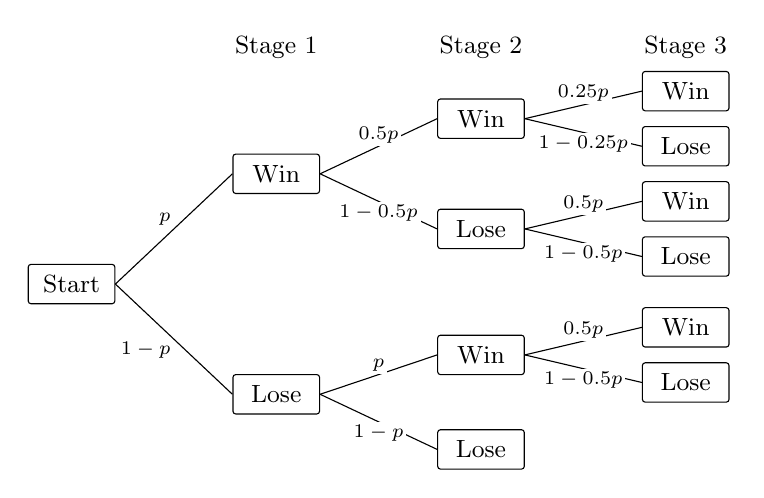
\begin{tikzpicture}[font=\small,
 bx/.style={draw,rounded corners=1pt,minimum width=1.1cm,minimum height=0.5cm,inner sep=1pt},
 lab/.style={font=\scriptsize,fill=white,inner sep=1pt}]
\node at (2.6,3.0){Stage 1};\node at (5.2,3.0){Stage 2};\node at (7.8,3.0){Stage 3};
\node[bx] (S) at (0,0){Start};
\node[bx] (W) at (2.6,1.4){Win};\node[bx] (L) at (2.6,-1.4){Lose};
\node[bx] (WW) at (5.2,2.1){Win};\node[bx] (WL) at (5.2,0.7){Lose};
\node[bx] (LW) at (5.2,-0.9){Win};\node[bx] (LL) at (5.2,-2.1){Lose};
\node[bx] (a1) at (7.8,2.45){Win};\node[bx] (a2) at (7.8,1.75){Lose};
\node[bx] (b1) at (7.8,1.05){Win};\node[bx] (b2) at (7.8,0.35){Lose};
\node[bx] (c1) at (7.8,-0.55){Win};\node[bx] (c2) at (7.8,-1.25){Lose};
\draw (S.east)--(W.west) node[midway,above left,lab]{$p$};
\draw (S.east)--(L.west) node[midway,below left,lab]{$1-p$};
\draw (W.east)--(WW.west) node[midway,above,lab]{$0.5p$};
\draw (W.east)--(WL.west) node[midway,below,lab]{$1-0.5p$};
\draw (L.east)--(LW.west) node[midway,above,lab]{$p$};
\draw (L.east)--(LL.west) node[midway,below,lab]{$1-p$};
\draw (WW.east)--(a1.west) node[midway,above,lab]{$0.25p$};
\draw (WW.east)--(a2.west) node[midway,below,lab]{$1-0.25p$};
\draw (WL.east)--(b1.west) node[midway,above,lab]{$0.5p$};
\draw (WL.east)--(b2.west) node[midway,below,lab]{$1-0.5p$};
\draw (LW.east)--(c1.west) node[midway,above,lab]{$0.5p$};
\draw (LW.east)--(c2.west) node[midway,below,lab]{$1-0.5p$};
\end{tikzpicture}\end{center}
\pt{(b)} $p(0.5p)\left(0.5^{2}p\right)>0.1$\par
$p^{3}>0.8$\par
$p>0.928$\par\smallskip
\pt{(c)} $\Pp{\text{wins exactly 2 stages out of 3}\mid\text{proceeds to Stage 3}}$\par
$=\dfrac{\Pp{\text{wins exactly 2 stages out of 3}\cap\text{proceeds to Stage 3}}}{\Pp{\text{proceeds to Stage 3}}}$\par
$=\dfrac{0.9(0.45)(1-0.225)+0.9(0.55)(0.45)+0.1(0.9)(0.45)}{1-(0.1)(0.1)}$\par
$=\dfrac{0.577125}{0.99}=0.583$

}
%Q 6|CJC 2024 Prelim P2 Q10(b)|Venn diagram: range of values of a probability
\defQ{6}{}{%
\begin{qparts}
\pt{(a)} In a certain university, there are 110 Co-Curricular Activities (CCAs) clustered into 4 categories. There are 22 Arts and Culture CCAs, 16 Community Service CCAs, 38 Physical Sports CCAs and 34 Special Interest CCAs.
\begin{qparts}
\pt{(i)} Albert wishes to find out about approaches to training of the Physical Sports CCAs, so he sends a questionnaire to 22 Physical Sports CCAs. Explain whether these 22 Physical Sports CCAs form a sample or a population. \mk{1}
\pt{(ii)} Benedict wishes to investigate the level of student engagement in CCAs, but does not want to obtain the detailed information necessary from all 110 CCAs. Explain how he should carry out his investigation, and why he should do the investigation in this way. \mk{2}
\pt{(iii)} Find the number of different possible samples of 16 CCAs, with 4 CCAs chosen from each category. \mk{2}
\end{qparts}
\pt{(b)} The probability of events $A$, $B$ and $C$ occurring are given by $\Pp{A}=\dfrac{8}{25}$, $\Pp{B}=\dfrac{61}{100}$ and $\Pp{C}=\dfrac{7}{20}$ respectively. It is also known that $\Pp{A\cap C}=\dfrac{11}{100}$, $\Pp{B\mid C}=\dfrac{13}{35}$ and $\Pp{A\cap B\cap C}=\dfrac{7}{100}$.
\begin{qparts}
\pt{(i)} Find $\Pp{B\cap C}$. \mk{2}
\pt{(ii)} If events $A$ and $B$ are independent, find $\Pp{A\cap B\cap C'}$. \mk{2}
\pt{(iii)} If events $A$ and $B$ are \textbf{not} known to be independent, find the greatest and least possible values of $\Pp{A\cap B\cap C'}$. \mk{4}
\end{qparts}
\end{qparts}
\src{CJC 2024 Prelim P2 Q10}}
\defS{6}{%
\pt{(a)(i)} These 22 CCAs form a sample since this number is less than the population size of Physical Sports CCAs which is 38.
\pt{(a)(ii)} Benedict should select a \underline{random sample} from the 110 CCAs: every CCA has an equal probability to be selected to be in the sample and the CCAS are selected independently. (If define without stating ``random'', need 2 full points.)\par
A random sample helps to \underline{avoid bias}.
\pt{(a)(iii)} Number of samples $={}^{22}C_{4}\times{}^{16}C_{4}\times{}^{38}C_{4}\times{}^{34}C_{4}$\par
$=4.56\times10^{16}$ (3 sf)
\pt{(b)(i)} $\Pp{B\mid C}=\dfrac{13}{35}$\par
$\dfrac{\Pp{B\cap C}}{\Pp{C}}=\dfrac{13}{35}$\par
$\dfrac{\Pp{B\cap C}}{\frac{7}{20}}=\dfrac{13}{35}$\par
$\Pp{B\cap C}=\dfrac{13}{100}$\par\smallskip
\pt{(b)(ii)} $\Pp{A\cap B}=\Pp{A}\times\Pp{B}$\par
$=\dfrac{8}{25}\times\dfrac{61}{100}$\par
$=\dfrac{122}{625}$\par
$\Pp{A\cap B\cap C'}$\par
$=\dfrac{122}{625}-\dfrac{7}{100}$\par
$=\dfrac{313}{2500}$\par\smallskip
\pt{(b)(iii)} \par
\begin{center}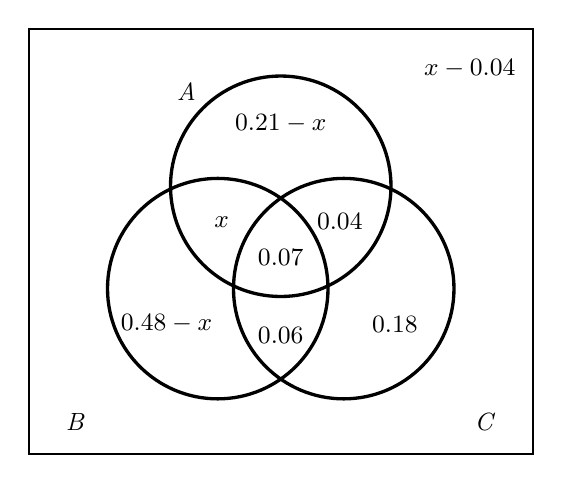
\begin{tikzpicture}[font=\small]
\draw[thick] (-3.2,-2.6) rectangle (3.2,2.8);
\draw[very thick] (0,0.8) circle (1.4);
\draw[very thick] (-0.8,-0.5) circle (1.4);
\draw[very thick] (0.8,-0.5) circle (1.4);
\node at (-1.2,2.0){\textit{A}};\node at (-2.6,-2.2){\textit{B}};\node at (2.6,-2.2){\textit{C}};
\node at (2.4,2.3){$x-0.04$};
\node at (0,1.6){$0.21-x$};
\node at (-0.75,0.35){$x$};
\node at (0.75,0.35){$0.04$};
\node at (0,-0.1){$0.07$};
\node at (-1.45,-0.95){$0.48-x$};
\node at (0,-1.1){$0.06$};
\node at (1.45,-0.95){$0.18$};
\end{tikzpicture}\end{center}
\noindent Let $\Pp{A\cap B\cap C'}=x$ where $0\leqslant x\leqslant1\ldots(1)$\par
\noindent Then\par
\noindent$\Pp{A\cap B'\cap C'}=\dfrac{8}{25}-\dfrac{11}{100}-x=\dfrac{21}{100}-x$\par\smallskip
\noindent$\Pp{A'\cap B\cap C'}=\dfrac{61}{100}-\dfrac{13}{100}-x=\dfrac{12}{25}-x$\par\smallskip
\noindent$\Pp{A\cup B\cup C}$\par
\noindent$=\Pp{C}+\Pp{A\cap B'\cap C'}+\Pp{A'\cap B\cap C'}+\Pp{A\cap B\cap C'}$\par
\noindent$=\dfrac{7}{20}+\left(\dfrac{21}{100}-x\right)+\left(\dfrac{12}{25}-x\right)+x$\par
\noindent$=\dfrac{26}{25}-x$\par\smallskip
\noindent Consider the probabilities $\Pp{A\cap B'\cap C'}$, $\Pp{A'\cap B\cap C'}$ and $\Pp{A\cup B\cup C}$,\par
\noindent$0\leqslant\dfrac{21}{100}-x\leqslant1$ \quad and \quad $0\leqslant\dfrac{12}{25}-x\leqslant1$ \quad and \quad $0\leqslant\dfrac{26}{25}-x\leqslant1$\par
\noindent$-\dfrac{79}{100}\leqslant x\leqslant\dfrac{21}{100}\ldots(2)$ \qquad $-\dfrac{13}{25}\leqslant x\leqslant\dfrac{12}{25}\ldots(3)$ \qquad $\dfrac{1}{25}\leqslant x\leqslant\dfrac{26}{25}\ldots(4)$\par\smallskip
\noindent Taking intersection of inequalities (1) to (4), $\dfrac{1}{25}\leqslant x\leqslant\dfrac{21}{100}$\par
\noindent$\min\Pp{A\cap B\cap C'}=\dfrac{1}{25}$ and $\max\Pp{A\cap B\cap C'}=\dfrac{21}{100}$

}
%Q 7|ACJC 2023 Prelim P2 Q9(a)|Sum to infinity of a GP
\defQ{7}{}{%
A bag contains one green disc, $r$ red discs and $2r$ blue discs, where $r>1$.
\begin{qparts}
\pt{(a)} Tim and Sim play a game by taking turns to draw a disc from the bag at random. The drawn disc is replaced after each turn. The first person to draw the green disc wins. If Sim started the game first, show that the probability of Sim winning the game is $\dfrac{3r+1}{6r+1}$. \mk{2}
\pt{(b)} In another game, a player draws 2 discs from the bag at random. If he draws a red disc, he scores 5 points, if he draws a blue disc, he scores 2 points and if he draws a green disc he scores 0. The player's score, denoted by $T$, is found by taking the difference in the number of points he scores for the two discs.
\begin{qparts}
\pt{(i)} Find $\mathrm{P}(T=t)$ for all possible values of $t$, leaving your answers in terms of $r$. \mk{3}
\pt{(ii)} Show that the expectation of the player's score is $\dfrac{2(2r+3)}{3r+1}$. \mk{1}
\end{qparts}
\pt{(c)} In a third game, a player draws a disc from the bag at random. If he draws a green disc, he wins \$0.15, if he draws a blue disc, he wins \$0.10 and if he draws a red disc, he loses \$0.25. May and Jun each draws a disc from the bag once, with the disc replaced in the bag after the first player drew. The probability that May ends up with more money than Jun is $\dfrac{27}{112}$. Find the value of $r$. \mk{2}\par
Is the game fair for a player? Explain. \mk{1}
\end{qparts}
\src{ACJC 2023 Prelim P2 Q9}}
\defS{7}{%
\pt{(a)} $\dfrac{1}{3r+1}+\left(\dfrac{3r}{3r+1}\right)^{2}\times\dfrac{1}{3r+1}+\left(\dfrac{3r}{3r+1}\right)^{4}\times\dfrac{1}{3r+1}+\ldots$\par\smallskip
$=\dfrac{\frac{1}{3r+1}}{1-\left(\frac{3r}{3r+1}\right)^{2}}=\dfrac{3r+1}{6r+1}$
\pt{(b)(i)} $\mathrm{P}(T=0)=\dfrac{r}{3r+1}\times\dfrac{r-1}{3r}+\dfrac{2r}{3r+1}\times\dfrac{2r-1}{3r}=\dfrac{5r-3}{3(3r+1)}$\par
$\mathrm{P}(T=2)=\dfrac{2r}{3r+1}\times\dfrac{1}{3r}\times2!=\dfrac{4}{3(3r+1)}$\par
$\mathrm{P}(T=3)=\dfrac{2r}{3r+1}\times\dfrac{r}{3r}\times2!=\dfrac{4r}{3(3r+1)}$\par
$\mathrm{P}(T=5)=\dfrac{r}{3r+1}\times\dfrac{1}{3r}\times2!=\dfrac{2}{3(3r+1)}$\par
{\renewcommand{\arraystretch}{1.6}\begin{tabular}{|c|c|c|c|c|}\hline $t$ & 0 & 2 & 3 & 5\\\hline $\mathrm{P}(T=t)$ & $\dfrac{5r-3}{3(3r+1)}$ & $\dfrac{4}{3(3r+1)}$ & $\dfrac{4r}{3(3r+1)}$ & $\dfrac{2}{3(3r+1)}$\\\hline\end{tabular}}
\pt{(b)(ii)} $\mathrm{E}(T)=\sum t\mathrm{P}(T=t)$\par
$=0\times\dfrac{5r-3}{3(3r+1)}+2\times\dfrac{4}{3(3r+1)}+3\times\dfrac{4r}{3(3r+1)}+5\times\dfrac{2}{3(3r+1)}$\par
$=\dfrac{8+12r+10}{3(3r+1)}=\dfrac{2(2r+3)}{3r+1}$
\pt{(c)} {\renewcommand{\arraystretch}{1.6}\begin{tabular}{|c|c|c|c|}\hline $x$ & $-0.25$ & 0.10 & 0.15\\\hline $\mathrm{P}(X=x)$ & $\dfrac{r}{3r+1}$ & $\dfrac{2r}{3r+1}$ & $\dfrac{1}{3r+1}$\\\hline\end{tabular}}\par
$\mathrm{P}(X_1>X_2)=\mathrm{P}(X_1=0.15,X_2=-0.25)$\par
$\qquad+\mathrm{P}(X_1=0.15,X_2=0.10)$\par
$\qquad+\mathrm{P}(X_1=0.10,X_2=-0.25)$\par
$\dfrac{2r^2+3r}{(3r+1)^2}=\dfrac{27}{112}$\par
$19r^2-174r+27=0$\par
$r=\dfrac{3}{19}\approx0.15789$ (rejected) \qquad $\therefore r=9$\par\medskip
$\mathrm{E}(X)=\sum x\mathrm{P}(X=x)$\par
$=-0.25\times\dfrac{9}{28}+0.10\times\dfrac{18}{28}+0.15\times\dfrac{1}{28}$\par
$=-0.010714\approx-0.0107$\par
Since $\mathrm{E}(X)<0$, the game is \underline{not} fair for a player, as he/she will be expected to lose 1.07 cents every time he/she plays.
}

%Q 8|HCI 2025 Prelim P2 Q6|Contextual probability
\defQ{8}{}{%
A basketball free throw game involves a team of two players, Ben and John. The game consists of at most three throws and the moment a player makes a successful shot, the team wins, and the game will end.\par
\noindent The game uses the following rules.
\begin{itemize}[leftmargin=3em,nosep]
\item Only one player is selected for each game and the probability that Ben is selected in a game is 0.7.
\item The probabilities that Ben and John make a successful shot in any single attempt are 0.1 and 0.07 respectively.
\item The shots are independent of each other.
\end{itemize}
\begin{qparts}
\pt{(a)} Find the probability that the team wins the game. \mk{3}
\pt{(b)} The team did not win the game. Find the probability that John was the one who was selected to shoot. \mk{3}
\pt{(c)} The team attempts the game repeatedly until the first game is won. Find the least number of attempts required such that the probability of winning within $n$ games is at least 0.95. \mk{2}
\end{qparts}
\src{HCI 2025 Prelim P2 Q6}}
\defS{8}{%
\pt{(a)} $\mathrm{P(wins)}$\par
$=\mathrm{P(wins\ and\ Ben\ selected)}+\mathrm{P(wins\ and\ John\ selected)}$\par
$=\mathrm{P(wins\mid Ben\ selected)P(Ben\ selected)}$\par
$\phantom{=}+\mathrm{P(wins\mid John\ selected)P(John\ selected)}$\par
$=\left(0.1+0.9\times0.1+0.9^{2}\times0.1\right)(0.7)$\par
$\phantom{=}+\left(0.07+0.93\times0.07+0.93^{2}\times0.07\right)(0.3)$\par
$=0.2483929$\par
OR\par
$\mathrm{P(wins)}$\par
$=\mathrm{P(wins\ and\ Ben\ selected)}+\mathrm{P(wins\ and\ John\ selected)}$\par
$=\mathrm{P(wins\mid Ben\ selected)P(Ben\ selected)}+$\par
$\phantom{=}\mathrm{P(wins\mid John\ selected)P(John\ selected)}$\par
$=\left(1-0.9^{3}\right)(0.7)+\left(1-0.93^{3}\right)(0.3)$\par
$=0.2483929$\par\smallskip
\pt{(b)} $\mathrm{P(John\ selected\mid did\ not\ win)}$\par
$=\dfrac{\mathrm{P(John\ selected\ and\ did\ not\ win)}}{\mathrm{P(did\ not\ win)}}$\par
$=\dfrac{0.3\times0.93^{3}}{1-0.2483929}$\par
$=0.321\ \text{(3sf)}$\par\smallskip
\pt{(c)} Required probability $=1-$ P(did not win in all $n$ games)\par
$=1-(1-0.2483929)^{n}$\par
OR\par
Required probability\par
$=$ P(win in 1st game) $+$ P(win in 2nd game)\par
$+$ P(win in 3rd game) $+\ldots+$ P(win in $n$\textsuperscript{th} game)\par
$=0.2483929+(1-0.2483929)(0.2483929)$\par
$+(1-0.2483929)^{2}(0.2483929)+\ldots$\par
$+(1-0.2483929)^{n-1}(0.2483929)$\par
$=\dfrac{0.2483929\left(1-(1-0.2483929)^{n}\right)}{1-(1-0.2483929)}$\par
$=1-(1-0.2483929)^{n}$\par\smallskip
$1-(1-0.2483929)^{n}\geqslant0.95$\par
$(1-0.2483929)^{n}\leqslant0.05$\par
\begin{tabular}{|c|c|}\hline $n$ & $(1-0.2483929)^{n}$\\\hline 10 & $0.0575>0.05$\\\hline 11 & $0.0432<0.05$\\\hline\end{tabular}\par
Smallest $n$ is 11.


}
%Q 9|ACJC 2025 Prelim P2 Q8|Unknowns in the table; solving simultaneously
\defQ{9}{}{%
The probability distribution of a discrete random variable $X$ is given as follows:
\begin{center}\begin{tabular}{|c|c|c|c|c|c|}\hline $x$ & $-2$ & $-1$ & 0 & 1 & 3\\\hline $\Pp{X=x}$ & 0.1 & $a$ & 0.3 & $b$ & $c$\\\hline\end{tabular}\end{center}
Given that $\mathrm{E}(X)=0.9$ and $\mathrm{Var}(X)=2.99$, find the values of $a$, $b$ and $c$. \mk{5}
\src{ACJC 2025 Prelim P2 Q8}}
\defS{9}{%
$\mathrm{E}(X)=(-2)(\tfrac{1}{10})+(-1)(a)+(0)(\tfrac{3}{10})+(1)(b)+(3)(c)$\par
$\dfrac{9}{10}=-\dfrac{2}{10}-a+b+3c$\par
$-a+b+3c=\dfrac{11}{10}$ \quad\dotfill(1)\par
$\mathrm{E}(X^2)=(-2)^2(\tfrac{1}{10})+(-1)^2(a)+(0)^2(\tfrac{3}{10})+(1)^2(b)+(3)^2(c)=\dfrac{4}{10}+a+b+9c$\par
$\mathrm{Var}(X)=\mathrm{E}(X^2)-[\mathrm{E}(X)]^2$\par
$\dfrac{299}{100}=\left(\dfrac{4}{10}+a+b+9c\right)-\left(\dfrac{9}{10}\right)^2$\par
$a+b+9c=\dfrac{34}{10}$ \quad\dotfill(2)\par
$\sum\Pp{X=x}=1$\par
$\dfrac{1}{10}+a+\dfrac{3}{10}+b+c=1$\par
$a+b+c=\dfrac{6}{10}$ \quad\dotfill(3)\par
Solving (1), (2) and (3), we have $a=\dfrac{1}{10}$ or 0.1, $b=\dfrac{3}{20}$ or 0.15, $c=\dfrac{7}{20}$ or 0.35

}
%Q 10|ASRJC 2025 Prelim P2 Q7|Fair game
\defQ{10}{}{%
Anthony plays a game using a four-sided fair die with the numbers 1, 2, 3 and 4 printed on its sides. Anthony rolls the die and should the outcome be a prime number, he wins an amount equivalent to that number in dollars. Conversely, if the outcome is a non-prime number, Anthony will lose an amount equivalent to that number in dollars. The random variable $X$ represents the amount of money Anthony wins in a roll of the die.
\begin{qparts}
\pt{(a)} Tabulate the probability distribution of $X$ and find the value of $\mathrm{E}(X)$. \mk{2}
\pt{(b)} Find the value of the variance of $X$. \mk{1}
\pt{(c)} The random variables $X_1$ and $X_2$ are two independent observations of $X$. By drawing a table of outcomes for $|X_1+X_2|$ or otherwise, find $\mathrm{E}(|X_1+X_2|)$. \mk{2}
\end{qparts}
Assume now that a biased six-sided die with numbers 2, 3, 4, 5, 6 and 7 printed on its sides, is used instead for the same game. It is known that for this biased die, the probability of obtaining a ``3'' is $p$, the probability of obtaining a ``5'' is $2p$ and the remaining four numbers each have an equal probability of occurring.
\begin{qparts}
\pt{(d)} Find the exact value of $p$ for the game to be fair using the biased die. \mk{3}
\end{qparts}
\src{ASRJC 2025 Prelim P2 Q7}}
\defS{10}{%
\pt{(a)} \begin{tabular}{|c|c|c|c|c|}\hline $x$ & $-4$ & $-1$ & 2 & 3\\\hline $\Pp{X=x}$ & $\frac14$ & $\frac14$ & $\frac14$ & $\frac14$\\\hline\end{tabular}\quad
$\mathrm{E}(X)=\dfrac{-4}{4}+\dfrac{-1}{4}+\dfrac{2}{4}+\dfrac{3}{4}=0$\par\smallskip
\pt{(b)} $\mathrm{Var}(X)=\left[\dfrac{(-4)^2}{4}+\dfrac{(-1)^2}{4}+\dfrac{2^2}{4}+\dfrac{3^2}{4}\right]-0^2=\dfrac{15}{2}$\par\smallskip
\pt{(c)} Let $Y=|X_1+X_2|$\par
\begin{tabular}{|c|c|c|c|c|}\hline $X_2\backslash X_1$ & $-4$ & $-1$ & 2 & 3\\\hline $-4$&8&5&2&1\\\hline $-1$&5&2&1&2\\\hline 2&2&1&4&5\\\hline 3&1&2&5&6\\\hline\end{tabular}\quad
\begin{tabular}{|c|c|c|c|c|c|c|}\hline $y$&1&2&4&5&6&8\\\hline $\Pp{Y=y}$&$\frac{4}{16}$&$\frac{5}{16}$&$\frac{1}{16}$&$\frac{4}{16}$&$\frac{1}{16}$&$\frac{1}{16}$\\\hline\end{tabular}\par
$\mathrm{E}(Y)=\dfrac{4}{16}+2\left(\dfrac{5}{16}\right)+4\left(\dfrac{1}{16}\right)+5\left(\dfrac{4}{16}\right)+6\left(\dfrac{1}{16}\right)+8\left(\dfrac{1}{16}\right)=\dfrac{13}{4}$\par\smallskip
\pt{(d)} The new probability distribution for $X$ is as tabulated below:\par
\begin{tabular}{|c|c|c|c|c|c|c|}\hline $x$&$-6$&$-4$&2&3&5&7\\\hline $\Pp{X=x}$&$\frac{1-3p}{4}$&$\frac{1-3p}{4}$&$\frac{1-3p}{4}$&$p$&$2p$&$\frac{1-3p}{4}$\\\hline\end{tabular}\par
$\mathrm{E}(X)=-6\left(\dfrac{1-3p}{4}\right)-4\left(\dfrac{1-3p}{4}\right)+2\left(\dfrac{1-3p}{4}\right)+3p+10p+7\left(\dfrac{1-3p}{4}\right)=-\left(\dfrac{1-3p}{4}\right)+13p=-\dfrac14+\dfrac{55}{4}p$\par
For the game to be fair, $-\dfrac14+\dfrac{55}{4}p=0$\par
Hence $p=\dfrac{1}{55}$

}
%Q 11|CJC 2024 Prelim P2 Q5|Total of two games (not CLT)
\defQ{11}{}{%
Andrea participates in a game show. In each round of the game, Andrea responds to a series of questions until she answers a question wrongly or she has answered five questions correctly. She is awarded one point for every correct answer and is awarded an additional 3 bonus points if she answers all five questions correctly. It is given that she answers each question independently and the probability she answers each question correctly is $\dfrac45$.
\begin{qparts}
\pt{(a)} Show that the probability that Andrea obtains 2 points in one round of the game is $\dfrac{16}{125}$. \mk{1}
\pt{(b)} Find the probability distribution of the points that Andrea obtains in one round of the game. \mk{2}
\pt{(c)} Find the expectation and variance of the points that Andrea obtains in one round of the game. \mk{2}
\pt{(d)} Find the probability that Andrea obtains less than 3 points after two rounds of the game. \mk{3}
\end{qparts}
\src{CJC 2024 Prelim P2 Q5}}
\defS{11}{%
\pt{(a)} Probability that Andrea obtains 2 points in a round of the game $=\left(\dfrac45\right)\left(\dfrac45\right)\left(\dfrac15\right)=\dfrac{16}{125}$\par\smallskip
\pt{(b)} Let $X$ be the random variable denoting the number of points obtained in a round.\par
{\renewcommand{\arraystretch}{1.6}\begin{tabular}{|c|c|c|c|c|c|c|}\hline $x$&0&1&2&3&4&8\\\hline $\Pp{X=x}$&$\frac15$&$\frac{4}{25}$&$\frac{16}{125}$&$\frac{64}{625}$&$\frac{256}{3125}$&$\frac{1024}{3125}$\\\hline\end{tabular}}\par\smallskip
\pt{(c)} \textbf{Method 1}: Using G.C., Expectation $=3.67232$ (exact); Variance $=3.22334^2=10.4$ (3 s.f.)\par
\textbf{Method 2}: $\mathrm{E}(X)=0\left(\frac15\right)+1\left(\frac{4}{25}\right)+2\left(\frac{16}{125}\right)+3\left(\frac{64}{625}\right)+4\left(\frac{256}{3125}\right)+8\left(\frac{1024}{3125}\right)=3.67232$\par
$\mathrm{E}(X^2)=0^2\left(\frac15\right)+1^2\left(\frac{4}{25}\right)+2^2\left(\frac{16}{125}\right)+3^2\left(\frac{64}{625}\right)+4^2\left(\frac{256}{3125}\right)+8^2\left(\frac{1024}{3125}\right)=23.87584$\par
$\mathrm{Var}(X)=\mathrm{E}(X^2)-[\mathrm{E}(X)]^2=23.87584-(3.67232)^2=10.4$ (to 3 s.f.)\par\smallskip
\pt{(d)} Probability that Andrea obtains less than 3 points after two rounds\par
$=\Pp{X_1+X_2<3}=\Pp{X_1+X_2=0}+\Pp{X_1+X_2=1}+\Pp{X_1+X_2=2}$\par
$=\Pp{X_1=0\cap X_2=0}+2\Pp{X_1=0\cap X_2=1}+2\Pp{X_1=0\cap X_2=2}+\Pp{X_1=1\cap X_2=1}$\par
$=\left(\frac15\right)^2+2\left(\frac15\right)\left(\frac{4}{25}\right)+2\left(\frac15\right)\left(\frac{16}{125}\right)+\left(\frac{4}{25}\right)^2=\dfrac{113}{625}$ or 0.1808 (exact)


}
%Q 12|SAJC DRV HW2 Review Q8|Expectation of a new variable (new table)
\defQ{12}{}{%
\noindent The number of muffins, $X$, bought by a randomly chosen customer at a muffin shop has probability distribution as shown in the table below:
\begin{center}\renewcommand{\arraystretch}{2.0}
\begin{tabular}{|c|c|c|c|c|c|c|c|}\hline
$x$ & 1 & 2 & 3 & 4 & 5 & 6 & $>6$\\\hline
$\Pp{X=x}$ & $\dfrac{1}{12}$ & $\dfrac{2}{12}$ & $\dfrac{3}{12}$ & $a$ & $\dfrac{2}{12}$ & $\dfrac{1}{12}$ & 0\\\hline
\end{tabular}\end{center}
\begin{qparts}
\pt{(i)} Find the value of $a$.
\pt{(ii)} State the expected value of $X$.
\pt{(iii)} Evaluate the variance of $X$.
\end{qparts}
\noindent Initially, the shopkeeper charges \$2.50 for each muffin, which cost 50 cents to produce.
\begin{qparts}
\pt{(iv)} Using the answer to part (ii), or otherwise, find the expected profit made per customer.
\end{qparts}
\noindent The shopkeeper decides to promote the sale of muffins by giving a free muffin to all customers who buy 4 or more muffins. As a result, the probability distribution of the number of muffins, $Y$, taken away by a customer is given in the following table.
\begin{center}\renewcommand{\arraystretch}{2.0}
\begin{tabular}{|c|c|c|c|c|c|c|c|}\hline
$y$ & 1 & 2 & 3 & 4 & 5 & 6 & $>6$\\\hline
$\Pp{Y=y}$ & $\dfrac{3}{36}$ & $\dfrac{4}{36}$ & $\dfrac{3}{36}$ & 0 & $\dfrac{20}{36}$ & $\dfrac{6}{36}$ & 0\\\hline
\end{tabular}\end{center}
\begin{qparts}
\pt{(v)} Find the expected profit made per customer.
\pt{(vi)} If the number of customers increases by 8\%, is the promotion more profitable for the shopkeeper? Give a reason for your answer.
\end{qparts}
\src{SAJC DRV HW2 Review Q8}}
\defS{12}{%
\pt{(i)} $\dfrac14$
\pt{(ii)} $3.5$
\pt{(iii)} $1\dfrac{11}{12}$
\pt{(iv)} {\color{gray}\itshape No official answer is printed for this part.}
\pt{(v)} \$6.86
\pt{(vi)} {\color{gray}\itshape No official answer is printed for this part.}
}
%NOSOL
%Q 13|JPJC 2025 Prelim P2 Q7|Central Limit Theorem
\defQ{13}{}{%
In a game, a player selects one ball at random from a bag which contains four balls numbered `1', `1', `2' and `3'. The player notes the number on the selected ball, and then tosses that number of fair coins. The number of heads obtained is denoted by $X$ and has a probability distribution as follows:
\begin{center}{\renewcommand{\arraystretch}{1.6}\begin{tabular}{|c|c|c|c|c|}\hline $x$&0&1&2&3\\\hline $\Pp{X=x}$&$a$&$\frac{15}{32}$&$b$&$\frac{1}{32}$\\\hline\end{tabular}}\end{center}
\begin{qparts}
\pt{(i)} Find the exact values of $a$ and $b$. \mk{3}
\pt{(ii)} Find $\mathrm{E}(X)$ and show that $\mathrm{Var}(X)=\dfrac{39}{64}$. \mk{2}
\pt{(iii)} The player plays 50 games. Find the probability that the average number of heads obtained per game exceed 1. \mk{2}
\end{qparts}
\src{JPJC 2025 Prelim P2 Q7}}
\defS{13}{%
\pt{(i)}\noindent\begin{minipage}[c]{0.55\linewidth}
$a=\Pp{X=0}=\left(\frac12\times\frac12\right)+\left(\frac14\times\left(\frac12\right)^2\right)+\left(\frac14\times\left(\frac12\right)^3\right)=\dfrac{11}{32}$\par
$b=\Pp{X=2}=\left(\frac14\times\left(\frac12\right)^2\right)+\left(\frac14\times{}^3C_2\times\left(\frac12\right)^3\right)=\dfrac{5}{32}$\par
Or $b=\Pp{X=2}=1-\frac{11}{32}-\frac{15}{32}-\frac{1}{32}=\frac{5}{32}$\par
$a=\dfrac{11}{32}$, $b=\dfrac{5}{32}$
\end{minipage}\hfill
\begin{minipage}[c]{0.42\linewidth}\centering
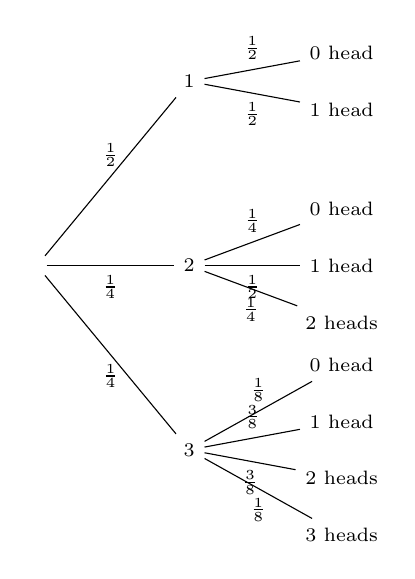
\begin{tikzpicture}[scale=0.9,font=\scriptsize,grow=right,level distance=2.15cm,
level 1/.style={sibling distance=2.6cm},level 2/.style={sibling distance=0.8cm}]
\node{}
 child{node{3}
   child{node{3 heads} edge from parent node[below]{$\frac18$}}
   child{node{2 heads} edge from parent node[below]{$\frac38$}}
   child{node{1 head} edge from parent node[above]{$\frac38$}}
   child{node{0 head} edge from parent node[above]{$\frac18$}}
   edge from parent node[below]{$\frac14$}}
 child{node{2}
   child{node{2 heads} edge from parent node[below]{$\frac14$}}
   child{node{1 head} edge from parent node[below]{$\frac12$}}
   child{node{0 head} edge from parent node[above]{$\frac14$}}
   edge from parent node[below]{$\frac14$}}
 child{node{1}
   child{node{1 head} edge from parent node[below]{$\frac12$}}
   child{node{0 head} edge from parent node[above]{$\frac12$}}
   edge from parent node[above]{$\frac12$}};
\end{tikzpicture}
\end{minipage}\par\smallskip
\pt{(ii)} Probability distribution of $X$:\ {\renewcommand{\arraystretch}{1.5}\begin{tabular}{|c|c|c|c|c|}\hline $x$&0&1&2&3\\\hline $\Pp{X=x}$&$\frac{11}{32}$&$\frac{15}{32}$&$\frac{5}{32}$&$\frac{1}{32}$\\\hline\end{tabular}}\par
$\mathrm{E}(X)=\sum x\Pp{X=x}=(0)\left(\frac{11}{32}\right)+(1)\left(\frac{15}{32}\right)+(2)\left(\frac{5}{32}\right)+(3)\left(\frac{1}{32}\right)=\dfrac78$\par
$\mathrm{E}(X^2)=\sum x^2\Pp{X=x}=(0)^2\left(\frac{11}{32}\right)+(1)^2\left(\frac{15}{32}\right)+(2)^2\left(\frac{5}{32}\right)+(3)^2\left(\frac{1}{32}\right)=\dfrac{11}{8}$\par
$\mathrm{Var}(X)=\mathrm{E}(X^2)-[\mathrm{E}(X)]^2=\dfrac{11}{8}-\left(\dfrac78\right)^2=\dfrac{39}{64}$ (Shown)\par\smallskip
\pt{(iii)} Let $X$ = number of heads obtained in one game; $\overline{X}$ = mean number of heads obtained per game\par
Since $n=50$ is large, by the Central Limit Theorem, $\overline{X}\sim\mathrm{N}\left(\dfrac78,\dfrac{39/64}{50}\right)=\mathrm{N}\left(\dfrac78,\dfrac{39}{3200}\right)$ approximately\par
$\Pp{\overline{X}>1}=0.12876\approx0.129$

}
%Q 14|ACJC 2025 Prelim P2 Q9|Double binomial
\defQ{14}{}{%
A fruit seller sources his oranges from a supplier with a large plantation where 1\% of the oranges are rotten. The supplier picks the oranges regardless of whether the oranges are rotten or not, and packs 20 oranges in each box at random.
\begin{qparts}
\pt{(a)} The random variable $X$ denotes the number of rotten oranges in a randomly chosen box. State in context two assumptions for $X$ to follow a binomial distribution. \mk{2}
\end{qparts}
Assume that $X$ follows a binomial distribution for the rest of this question.\par
The fruit seller considers a box containing between 2 and 5 rotten oranges inclusive as substandard.
\begin{qparts}
\pt{(b)} Find the probability that a randomly chosen box is substandard. \mk{1}
\pt{(c)} Find the expected number of rotten oranges in a box. \mk{1}
\end{qparts}
A truckload of 10 randomly chosen boxes of oranges is then sent to the fruit seller.
\begin{qparts}
\pt{(d)} Find the probability that not more than 2 boxes from the entire truckload are substandard. \mk{2}
\end{qparts}
Upon receiving the oranges, the fruit seller inspects the boxes with these conditions:
\begin{itemize}[leftmargin=2.2em]
\item Accept the entire truckload if the first box opened has no rotten oranges.
\item Reject the entire truckload if the first box opened has more than 1 rotten orange.
\item If the first box has exactly 1 rotten orange, the fruit seller opens a second box.
\item If the second box has at most 1 rotten orange, he will accept the entire truckload. Otherwise, he will reject the entire truckload.
\end{itemize}
\begin{qparts}
\pt{(e)} Find the probability that he will reject the entire truckload. \mk{2}
\end{qparts}
\src{ACJC 2025 Prelim P2 Q9}}
\defS{14}{%
\pt{(a)} The probability that an orange is rotten is a constant of 0.01.\par
Whether an orange is rotten is independent of whether any other oranges are rotten.\par\smallskip
\pt{(b)} Let the random variable $X$ denote the number of rotten oranges in a box of 20 oranges.\par
$X\sim\mathrm{B}(20,0.01)$\par
$\Pp{2\leqslant X\leqslant5}=\Pp{X\leqslant5}-\Pp{X\leqslant1}=0.0169$\par\smallskip
\pt{(c)} $\mathrm{E}(X)=(20)(0.01)=0.2$\par\smallskip
\pt{(d)} Let the random variable $Y$ denote the number of substandard boxes out of the entire truckload of 10 boxes.\par
$Y\sim\mathrm{B}(10,p)$ where $p=0.0169$\par
$\Pp{Y\leqslant2}=0.999$ (3 s.f.)\par\smallskip
\pt{(e)} Let $A$ = \{he rejects the entire truckload\}\par
$\mathrm{P}(A)=\Pp{X\geqslant2}+\Pp{X=1}\Pp{X\geqslant2}=[1-\Pp{X\leqslant1}]+\Pp{X=1}[1-\Pp{X\leqslant1}]=0.0196$

}
%Q 15|YIJC 2024 Prelim P2 Q8|The $k$th trial is the $m$th success
\defQ{15}{}{%
A manufacturer produces a large number of tumblers of three colours: black, pink and white in the respective ratios $3:2:1$. The tumblers are packed into boxes of 20 each.\par
Assume that the number of white tumblers in each box follows a binomial distribution.
\begin{qparts}
\pt{(a)} Find the probability that the number of white tumblers in a randomly chosen box is between 4 and 9 inclusive. \mk{2}
\pt{(b)} Find the probability that the 19th tumbler chosen from the box is the fourth white tumbler. \mk{2}
\end{qparts}
It is known that, on average, $p$\,\% of the tumblers are defective. The number of defective tumblers in a box also follows a binomial distribution. The probability that a box contains at most one defective tumbler is 0.95.
\begin{qparts}
\pt{(c)} Write down an equation satisfied by $p$. Hence find the value of $p$. \mk{3}
\end{qparts}
\src{YIJC 2024 Prelim P2 Q8}}
\defS{15}{%
\pt{(a)} Let $X$ be the number of white tumblers in a box of 20. $X\sim\mathrm{B}(20,\frac16)$\par
$\Pp{4\leqslant X\leqslant9}=\Pp{X\leqslant9}-\Pp{X\leqslant3}\approx0.433$\par
Alternative: $\Pp{X=4}+\Pp{X=5}+\dots+\Pp{X=9}\approx0.433$\par\smallskip
\pt{(b)} Let $W$ be the number of white tumblers from 18 tumblers. $W\sim\mathrm{B}(18,\frac16)$\par
Required probability $=\Pp{W=3}\times\dfrac16\approx0.0409$\par\smallskip
\pt{(c)} Let $D$ be the number of defective tumblers in a box of 20. $D\sim\mathrm{B}(20,0.01p)$\par
$\Pp{D\leqslant1}=0.95$\par
$\Pp{D=0}+\Pp{D=1}=0.95$\par
${}^{20}C_0(0.01p)^0(1-0.01p)^{20}+{}^{20}C_1(0.01p)^1(1-0.01p)^{19}=0.95$\par
$(1-0.01p)^{20}+0.2p(1-0.01p)^{19}=0.95$\par
Using G.C., $p\approx1.81$

}
%Q 16|N2018 P2 Q6|Bug turning left and right
\defQ{16}{}{%
\begin{center}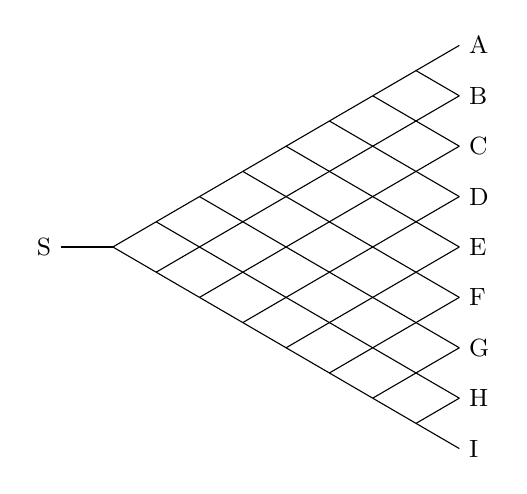
\begin{tikzpicture}[x=0.55cm,y=0.32cm,font=\small]
\draw (-1.2,0)--(0,0);
\foreach \i in {0,...,7}{\foreach \k in {0,...,\i}{
  \draw (\i,2*\k-\i)--(\i+1,2*\k-\i+1); \draw (\i,2*\k-\i)--(\i+1,2*\k-\i-1);}}
\node[left] at (-1.2,0){S};
\foreach \l [count=\j from 0] in {A,B,C,D,E,F,G,H,I}{\node[right] at (8,8-2*\j){\l};}
\end{tikzpicture}\end{center}
In a computer game, a bug moves from left to right through a network of connected paths. The bug starts at S and, at each junction, randomly takes the left fork with probability $p$ or the right fork with probability $q$, where $q=1-p$. The forks taken at each junction are independent. The bug finishes its journey at one of the 9 endpoints labelled A--I (see diagram).
\begin{qparts}
\pt{(i)} Show that the probability that the bug finishes its journey at D is $56p^5q^3$. \mk{2}
\pt{(ii)} Given that the probability that the bug finishes its journey at D is greater than the probability that the bug finishes its journey at any one of the other endpoints, find exactly the possible range of values of $p$. \mk{4}
\end{qparts}
In another version of the game, the probability that, at each junction, the bug takes the left fork is $0.9p$, the probability that the bug takes the right fork is $0.9q$ and the probability that the bug is swallowed up by a `black hole' is 0.1.
\begin{qparts}
\pt{(iii)} Find the probability that, in this version of the game, the bug reaches one of the endpoints A--I, without being swallowed up by a black hole. \mk{1}
\end{qparts}
\src{N2018 P2 Q6}}
\defS{16}{%
\pt{(i)} {\color{gray}\itshape No official answer is printed for this part.}
\pt{(ii)} $\dfrac59<p<\dfrac23$
\pt{(iii)} 0.430
}
%NOSOL
%Q 17|9758 Specimen Paper (for 2025) P2 Q7|Range of $p$ given the mode
\defQ{17}{}{%
`Crunchers' are sweets that are sold in packets of 8. Each packet is made up of randomly chosen coloured sweets. On average 15\% of Crunchers are yellow.
\begin{qparts}
\pt{(a)} Find the probability that a randomly chosen packet of Crunchers contains no more than one yellow sweet. \mk{2}
\pt{(b)} Kev buys 70 randomly chosen packets of Crunchers. Find the probability that at least 50 of these packets contain no more than one yellow sweet. \mk{3}
\end{qparts}
On average the proportion of Crunchers that are red is $p$. It is known that the modal number of red sweets in a packet is 3.
\begin{qparts}
\pt{(c)} Use this information to find exactly the range of values that $p$ can take. \mk{4}
\end{qparts}
\src{9758 Specimen Paper (for 2025) P2 Q7}}
\defS{17}{%
\pt{(a)} Use of B(8, 0.15);\quad 0.657\par
\pt{(b)} Use of B(70, 0.65718);\quad Use of $1-\mathrm{P}(x\leqslant49)$;\quad 0.190\par
\pt{(c)} $\dfrac{8\times7\times6}{1\times2\times3}p^3(1-p)^5>\dfrac{8\times7}{1\times2}p^2(1-p)^6$;\quad $p>\dfrac13$\par
$\dfrac{8\times7\times6}{1\times2\times3}p^3(1-p)^5>\dfrac{8\times7\times6\times5}{1\times2\times3\times4}p^4(1-p)^4$;\quad $p<\dfrac49$

}
%Q 18|TJC 2025 Prelim P2 Q7|Central Limit Theorem
\defQ{18}{}{%
A factory produces porcelain bowls. It is known that, on average, 8\% of the bowls are faulty. The bowls are packed in boxes of 20. A box is considered imperfect if it contains more than 2 faulty bowls. Assume that the number of faulty bowls in a box follows a binomial distribution.
\begin{qparts}
\pt{(a)} Find the probability that a randomly chosen box is imperfect. \mk{2}
\end{qparts}
These boxes are packed into cartons of 12 boxes each.
\begin{qparts}
\pt{(b)} Find the probability that, out of 3 randomly chosen cartons, there are 2 cartons that contain fewer than 15 faulty bowls each. \mk{3}
\end{qparts}
Let $Y$ be the number of imperfect boxes in a randomly chosen carton.
\begin{qparts}
\pt{(c)} State the values of $\mathrm{E}(Y)$ and $\mathrm{Var}(Y)$. \mk{2}
\pt{(d)} Hence using a suitable approximation, find the probability that the total number of imperfect boxes in a random sample of 35 cartons is at most 85. \mk{2}
\end{qparts}
\src{TJC 2025 Prelim P2 Q7}}
\defS{18}{%
\pt{(a)} Let $X$ be the number of faulty bowls in a box of 20 bowls. $X\sim\mathrm{B}(20,0.08)$\par
$\Pp{X>2}=1-\Pp{X\leqslant2}=1-0.78795=0.21205$ (5 s.f.) $=0.212$ (3 s.f.)\par\smallskip
\pt{(b)} Let $W$ be the number of faulty bowls in a carton (of 12 boxes). $W\sim\mathrm{B}(12\times20,0.08)$, i.e. $W\sim\mathrm{B}(240,0.08)$\par
$\Pp{W<15}=\Pp{W\leqslant14}=0.12933$ (5 s.f.)\par
Required Probability $={}^3C_2(0.12933)^2(1-0.12933)=0.0437$ (3 s.f.)\par
\textbf{OR} Let $A$ be the number of cartons out of 3 contains fewer than 15 faulty bowls each. $A\sim\mathrm{B}(3,0.12933)$\par
Required Probability $=\Pp{A=2}=0.0437$ (3 s.f.)\par\smallskip
\pt{(c)} $Y\sim\mathrm{B}(12,0.21205)$\par
$\mathrm{E}(Y)=np=12\times0.21205=2.5446=2.54$ (3 s.f.)\par
$\mathrm{Var}(Y)=np(1-p)=12\times0.21205\times(1-0.21205)=2.0050$ (5 s.f.) $=2.01$ (3s.f.)\par\smallskip
\pt{(d)} $Y\sim\mathrm{B}(12,0.21205)$. Let $T=Y_1+\dots+Y_{35}$.\par
Since sample size 35 is large, by Central Limit Theorem,\par
$T\sim\mathrm{N}(35\times2.5446,\,35\times2.0050)$ approximately\par
i.e. $T\sim\mathrm{N}(89.061,\,70.175)$ approximately\par
Required probability $=\Pp{T\leqslant85}=0.314$ (3 s.f.)


}
%Q 19|ASRJC 2025 Prelim P2 Q9|Combining independent normal variables
\defQ{19}{}{%
\textbf{In this question, you should state clearly all the distributions that you use, together with the values of the appropriate parameters.}\par
A toy designer creates weighted wooden blocks used in balance-based educational toys. There are two types of blocks: cylindrical blocks and cuboidal blocks. The mass, in grams, of each cylindrical block and cuboidal block follow a normal distribution with the following parameters:
\begin{center}\small\begin{tabular}{|l|c|c|}\hline & Mean & Standard Deviation\\\hline cylindrical block & 280 & 6\\\hline cuboidal block & 220 & 5\\\hline\end{tabular}\end{center}
\begin{qparts}
\pt{(a)} Find the probability that the mass of a randomly selected cylindrical block exceeds the mass of a randomly selected cuboidal block by more than 65 grams. \mk{2}
\pt{(b)} The probability that the total of twice the mass of a cylindrical block and thrice the mass of a cuboidal block being less than $M$ g is 0.355. Find the value of $M$, giving your answer to the nearest integer. \mk{2}
\end{qparts}
To build a deluxe seesaw model, the designer uses:
\begin{itemize}[leftmargin=3em,nosep]
\item 2 cylindrical blocks,
\item 3 cuboidal blocks,
\item 7 screws,
\item 1 wooden plank.
\end{itemize}
The blocks are drilled before assembly to fit screws:
\begin{itemize}[leftmargin=3em,nosep]
\item Each cylindrical block loses 5\% of its mass after drilling.
\item Each cuboidal block loses 3\% of its mass after drilling.
\end{itemize}
The masses of the remaining components follow a normal distribution with the following parameters:
\begin{center}\small\begin{tabular}{|l|c|c|}\hline & Mean & Standard Deviation\\\hline screw & 8 & 1.2\\\hline wooden plank & 540 & 8\\\hline\end{tabular}\end{center}
When assembling the deluxe seesaw model, all of its components are chosen at random.
\begin{qparts}
\pt{(c)} Find the probability that the total mass of all the modified components in a deluxe seesaw model is more than 1785 g. \mk{4}
\end{qparts}
\src{ASRJC 2025 Prelim P2 Q9}}
\defS{19}{%
\pt{(a)} Let $X$ and $Y$ be the mass of a randomly selected cylindrical and cuboidal block (in g) respectively.\par
$X\sim\mathrm{N}(280,\,6^2)$ \ and \ $Y\sim\mathrm{N}(220,\,5^2)$\par
$X-Y\sim\mathrm{N}(280-220,\,5^2+6^2)$\par
$X-Y\sim\mathrm{N}(60,\,61)$\par
$\mathrm{P}(X-Y>65)=0.261$
\pt{(b)} Let $C=2X+3Y$\par
$C\sim\mathrm{N}(2\times280+3\times220,\,2^2\times6^2+3^2\times5^2)$\par
$C\sim\mathrm{N}(1220,\,369)$\par
Given $\mathrm{P}(C<M)=0.355$\par
From GC, $M=1212.8568$\par
$M=1213$
\pt{(c)} Let $S$ and $W$ be the mass of a randomly selected screw and wooden plank (in g) respectively.\par
$S\sim\mathrm{N}(8,\,1.2^2)$ \ and \ $W\sim\mathrm{N}(540,\,8^2)$\par
Let $T=0.95(X_1+X_2)+0.97(Y_1+Y_2+Y_3)+S_1+\cdots+S_7+W$\par
$\mathrm{E}(T)=(0.95\times2\times280)+(0.97\times3\times220)+(7\times8)+540$\par
$\phantom{\mathrm{E}(T)}=532+426.8+56+540$\par
$\phantom{\mathrm{E}(T)}=1768.2$\par
$\mathrm{Var}(T)=(0.95^2\times2\times6^2)+(0.97^2\times3\times5^2)+(7\times1.2^2)+64$\par
$\phantom{\mathrm{Var}(T)}=64.98+70.5675+10.08+64$\par
$\phantom{\mathrm{Var}(T)}=209.6275$\par
$\mathrm{P}(T>1785)=0.123$
}
%Q 20|NJC 2024 Prelim P2 Q12|Sketching a normal curve
\defQ{20}{}{%
In this question you should state the parameters of any distribution you use.\par
An electric power service company keeps records of the installation time of its electricity meters in the houses in a new estate. The time taken to install an electricity meter is normally distributed with mean 45 minutes and standard deviation 6 minutes.
\begin{qparts}
\pt{(a)} Sketch the distribution for the installation time of an electricity meter between 20 minutes and 70 minutes. \mk{2}
\pt{(b)} A house that has its electricity meter take more than 1 hour to be installed is considered `inefficient'. The company randomly selects $n$ houses in the estate for quality control in their services. Find the greatest value of $n$ such that the probability that fewer than 3 of these $n$ houses are `inefficient' is at least 0.90. \mk{3}
\pt{(c)} Each month, the amount of electricity, in kilowatt-hours (kWh), used by a particular household in the estate has the distribution $\mathrm{N}(524,\,27^2)$. The company charges households for electricity used at \$0.26 per kWh and each household is billed every two months. Find the probability that a randomly chosen bill for this household is more than \$270 given that it is between \$250 and \$280. State an assumption that is needed for your calculations to be valid. \mk{4}
\pt{(d)} The company also installs gas meters in the houses in the estate. The time taken in minutes to install a gas meter follows a normal distribution. 40\% of the gas meters each has an installation time greater than 53 minutes and 15\% of the gas meters each has an installation time less than 38 minutes. Find the mean and standard deviation of the installation times of the gas meters in the estate. \mk{4}
\end{qparts}
\src{NJC 2024 Prelim P2 Q12}}
\defS{20}{%
\pt{(a)} Let $X$ denote the random variable `time taken (min) to install an electricity meter.'\par
$X\sim\mathrm{N}(45,6^2)$
\figNjcSketch
Note: $\mathrm{P}(20<X<70)=0.99997$
\pt{(b)} Let $E$ be the random variable `number of `inefficient' houses out of $n$ houses.'\par
$E\sim\mathrm{B}(n,\,\mathrm{P}(X>60))$\par
$E\sim\mathrm{B}(n,\,0.0062097)$\par
$\mathrm{P}(E<3)=\mathrm{P}(E\leq2)\geq0.90$\par
Using GC,\par
\begin{tabular}{|c|l|}\hline $n$ & $\mathrm{P}(E\leq2)$\\\hline 177 & $0.9012\ \geq0.9$\\\hline 178 & $0.8999\ <0.9$\\\hline 179 & 0.8986\\\hline\end{tabular}\par
Largest $n=177$
\pt{(c)} Let $W$ be the random variable `amount of electricity (kWh) used in the household in a month.'\par
$W\sim\mathrm{N}(524,\,27^2)$\par
Let $T=0.26(W_1+W_2)$.\par
$\mathrm{E}(T)=0.26\times524\times2=272.48$\par
$\mathrm{Var}(T)=0.26^2\times2\times27^2=98.5608$\par
$T\sim\mathrm{N}(272.48,\,98.5608)$\par
$\mathrm{P}\left(T>270\,\middle|\,250<T<280\right)=\dfrac{\mathrm{P}(270<T<280)}{\mathrm{P}(250<T<280)}$\par
$\phantom{\mathrm{P}\left(T>270\,|\,250<T<280\right)}=\dfrac{0.37425}{0.76383}$\par
$\phantom{\mathrm{P}\left(T>270\,|\,250<T<280\right)}=0.490$ \ (3 s.f.)\par
We need to assume that the electricity used in each of these two months is independent for this particular household.
\pt{(d)} Let $G$ denote the random variable `time taken (min) to install a gas meter\par
$G\sim\mathrm{N}(\mu,\sigma^2)$.\par
$\mathrm{P}(G<38)=0.15,\qquad\mathrm{P}(G>53)=0.4$\par
$\mathrm{P}\left(Z<\dfrac{38-\mu}{\sigma}\right)=0.15,\qquad\mathrm{P}\left(Z>\dfrac{53-\mu}{\sigma}\right)=0.4$\par
By G.C.,\par
$\dfrac{38-\mu}{\sigma}=-1.0364,\qquad\dfrac{53-\mu}{\sigma}=0.25335$\par
$\mu-1.0364\sigma=38---(1),\quad\mu+0.25335\sigma=53---(2)$\par
Solving (1) and (2):\par
$\mu=50.0535=50.1$ \ (3 s.f.)\par
$\sigma=11.6298=11.6$ \ (3 s.f.)
}
%Q 21|MI 2025 Prelim P2 Q6|invNorm simultaneous equations; $\mu$ by symmetry
\defQ{21}{}{%
The waiting times for customers to get their pastries from a popular bakery is modelled by a normal distribution with mean $\mu$ minutes and standard deviation $\sigma$ minutes. On average, 10\% of customers wait for more than 25 minutes and the same percentage of customers wait for less than 5 minutes.
\begin{qparts}
\pt{(i)} Find the values of $\mu$ and $\sigma$, leaving your answers to the nearest minute. \mk{3}
\pt{(ii)} Explain if the normal distribution is a suitable model for the waiting times for customers to get pastries from this bakery. \mk{1}
\end{qparts}
\src{MI 2025 Prelim P2 Q6}}
\defS{21}{%
\pt{(i)} Let $X$ be the waiting time to get pastries from the popular bakery of a randomly chosen customer. $X\sim\mathrm{N}(\mu,\,\sigma^2)$\par
Given $\mathrm{P}(X<5)=\mathrm{P}(X>25)=0.10$.\par
\underline{\textbf{Method 1}}\par
By symmetry, $\mu=\dfrac{5+25}{2}=15$
\figMiSym
$\mathrm{P}(X>25)=0.10$\par
$\mathrm{P}\left(Z>\dfrac{25-15}{\sigma}\right)=0.10$\par
$\dfrac{10}{\sigma}=1.28155$\par
$\sigma=7.80305$\par
{\color{black!50}\rule[0.5ex]{0.9\linewidth}{0.4pt}}\par
\textbf{\textit{Alternatively,}}\par
$\mathrm{P}(X>25)=0.10$\par
Using GC,
\figMiGC
$\sigma=7.80304$\par
{\color{black!50}\rule[0.5ex]{0.9\linewidth}{0.4pt}}\par
$\therefore\mu=15,\ \sigma=8$ (to the nearest minute).\par\medskip
\underline{\textbf{Method 2}}\par
\begin{tabular}{@{}l@{\qquad}l@{}}
$\mathrm{P}(X>25)=0.10$ & $\mathrm{P}(X<5)=0.10$\\[1ex]
$\mathrm{P}\left(Z>\dfrac{25-\mu}{\sigma}\right)=0.10$ & $\mathrm{P}\left(Z<\dfrac{5-\mu}{\sigma}\right)=0.10$\\[2.2ex]
$\dfrac{25-\mu}{\sigma}=1.28155$ & $\dfrac{5-\mu}{\sigma}=-1.28155$\\[2ex]
$\mu+1.28155\sigma=25$ \ldots\ (1) & $\mu-1.28155\sigma=5$ \ldots\ (2)
\end{tabular}\par\smallskip
Solving (1) and (2) simultaneously,\par
$\mu=15,\ \sigma=7.80305.$\par
$\therefore\mu=15,\ \sigma=8$ (to the nearest minute).
\pt{(ii)} Consider $X\sim\mathrm{N}(15,\,8^2)$.\par
$\mathrm{P}(X<0)=0.0304$. \ (or 0.02728 if we use $\sigma=7.80305$)\par
The waiting times cannot be negative but $\mathrm{P}(X<0)$ is about 3\%, which is not insignificant. Thus, the normal distribution is not a suitable model.\par\smallskip
\textbf{Note:}\par
For normal distribution:\par
$\mathrm{P}(\mu-3\sigma<X<\mu+3\sigma)\approx0.997$ i.e. 99.7\%.\par
Hence, whenever the probability of obtaining unreasonable values of $x$ exceeds 0.003, we can conclude that the normal distribution is not suitable
}
%Q 22|RVHS 2025 Prelim P2 Q12|Binomial count of a normal event
\defQ{22}{}{%
A factory produces metal discs and metal bars for constructing machinery parts. The mass of a randomly chosen metal disc follows a normal distribution with mean 18 grams and standard deviation 0.6 grams. The mass of a randomly chosen metal bar has an independent normal distribution with mean 20 grams and standard deviation $\sigma$ grams.
\begin{qparts}
\pt{(a)} Sketch the distribution for the masses of the metal disc between 14 grams and 22 grams. \mk{1}
\pt{(b)} 2 metal discs are randomly chosen. Find the probability that the mass of one of the discs is less than 19 grams and the other metal disc has mass more than 19 grams. \mk{2}
\pt{(c)} Find the range of values of $k$ such that less than 90\% of the metal discs have masses within $k$ grams of the mean mass of the metal discs. \mk{2}
\pt{(d)} It is known that 7.65\% of the metal bars have masses more than 21 grams. Find the value of $\sigma$. \mk{2}
\end{qparts}
It is given that $\sigma=0.5$ for the rest of the question.
\begin{qparts}
\pt{(e)} A client places an order for a new kind of metal strips. The metal strips are modelled as similar solids to the metal bars with a 20\% reduction in mass.\par
A production worker selects 8 of the metal strips for inspection. Find the probability that at least 5 of the metal strips have masses between 15.8 grams and 17.2 grams. \mk{3}
\pt{(f)} A protective case is designed for the safe transportation of the metal bar. Each metal bar is placed inside a protective case during transportation. The masses of the protective cases are modelled as 30\% of the masses of the metal bars.\par
Let $T$ denote the total mass of 4 of the metal bars and their protective cases. Find the variance of $T$. \mk{2}
\end{qparts}
\src{RVHS 2025 Prelim P2 Q12}}
\defS{22}{%
\pt{(a)} \figRvSketch
\pt{(b)} Let $D$ be the random variable denoting the mass of a randomly chosen metal disc.\par
$D\sim N(18,\,0.6^2)$\par
Probability required\par
$=\dbinom{2}{1}\left[P(D<19)\right]\left[P(D>19)\right]---(*)$\par
$=0.0910128294$\par
$\approx0.0910$ (3 s.f.)
\pt{(c)} $P(18-k<D<18+k)<0.9$\par
Since $P(17.01308782<D<18.98691218)=0.9$, then\par
$18+k<18.98691218$\par
$k<0.987$
\pt{(d)} 7.65\% of the metal bars have masses more than 21 grams.\par
Let $B$ be the random variable denoting the mass of a randomly chosen metal bar.\par
$B\sim N(20,\sigma^2)$\par
$P(B>21)=0.0765$\par
$P\left(Z>\dfrac{21-20}{\sigma}\right)=0.0765$\par
$P\left(Z>\dfrac{1}{\sigma}\right)=0.0765$\par
$\dfrac{1}{\sigma}=1.429014729$\par
$\sigma=0.6997$\par
$\sigma=0.700$ (3.s.f)
\pt{(e)} Let $S$ be the random variable denoting the mass of a randomly chosen metal strip.\par
$S=0.8B\sim N(0.8\times20,\,0.8^2\times0.5^2)$\par
$S\sim N(16,\,0.4^2)$\par
$P(15.8<S<17.2)=0.6901125632$\par
Let $X$ be the random variable denoting the number of metal strips whose mass lies between 15.8 grams and 17.2 grams, out of 8 strips.\par
$X\sim B(8,\,0.6901125632)$\par
$P(X\geq5)$\par
$=1-P(X\leq4)$\par
$=0.7875751008$\par
$\approx0.788$ (3.s.f)
\figRvBinom
\pt{(f)} Let $C$ be the random variable denoting the mass of a randomly chosen protective case.\par
$C\sim N(0.3\times20,\,0.3^2\times0.5^2)$\par
$C\sim N(6,\,0.15^2)$\par\smallskip
$B\sim N(20,\,0.5^2)$\par
Let $Y=B+C$\par
$Y\sim N(20+6,\,0.5^2+0.15^2)$\par
$Y\sim N(26,\,0.2725)$\par\smallskip
Let $T=Y_1+Y_2+Y_3+Y_4$\par
$\mathrm{Var}(T)=4\times0.2725$\par
$\phantom{\mathrm{Var}(T)}=1.09$ (3 s.f)\par\medskip
\underline{\textbf{Common Mistake}}\par
Let $C$ be the random variable denoting the mass of a randomly chosen protective case.\par
$C=0.3B$\par\smallskip
$B\sim N(20,\,0.5^2)$\par
Let $Y=B+C$\par
$Y=B+0.3B=1.3B$\par
$Y\sim N(1.3\times20,\,1.3^2\times0.5^2)$\par
$Y\sim N(26,\,0.4225)$\par\smallskip
Let $T=Y_1+Y_2+Y_3+Y_4$\par
$T\sim N(4\times26,\,4\times0.4225)$\par
$T\sim N(104,\,1.69)$
}
%Q 23|ACJC 2023 Prelim P2 Q11
\defQ{23}{}{%
Energy bars are a convenient source of nutrition for athletes. A typical energy bar weighs between 30-50 g and is likely to supply about 200-300 calories. An American company sells energy bars and a nutritionist working in the company claims that the mean number of calories in a product, Perfect Protein bars, is 350 calories.\par
A random sample of 30 bars is collected and the number of calories, $x$ cal, in the 30 bars is summarised as follows.
\[\textstyle\sum x=10446,\qquad \sum x^2=3638000.\]
\begin{qparts}
\pt{(i)} Test at the 3\% level of significance whether the mean number of calories in Perfect Protein bars is less than 350 calories, defining any symbols that you use. \mk{7}
\pt{(ii)} Explain why the test would be inadmissible if the nutritionist had taken a random sample of 15 energy bars and hence state an assumption needed for him to carry out the test. \mk{1}
\pt{(iii)} If the test was for whether the mean number of calories in Perfect Protein bars is 350 calories, find the smallest level of significance for which the nutritionist's claim will be rejected. \mk{2}
\end{qparts}
The company launched a new product called Dynamic Protein bars which are advertised to be higher in calories than Perfect Protein bars. A random sample of 45 Dynamic Protein bars is collected to test this and the mean number of calories of the sample is found to be 352.2.
\begin{qparts}
\pt{(iv)} The result of this investigation shows that there is no reason to believe that the mean number of calories in the new product is more than 350 calories at the 4\% level of significance. Find the range of possible values of the variance used in calculating the test statistic. \mk{3}
\end{qparts}
\src{ACJC 2023 Prelim P2 Q11}}
\defS{23}{%
\pt{(i)} $\bar{x}=\dfrac{\sum x}{n}=\dfrac{10446}{30}=348.2$ (exact)\par
$s^2=\dfrac{1}{n-1}\left(\sum x^2-\dfrac{\left(\sum x\right)^2}{n}\right)=\dfrac{1}{29}\left(3638000-\dfrac{(10446)^2}{30}\right)=24.23448$\par
Let $\mu$ be the population mean number of calories in Perfect Protein bars.\par\medskip
Null hypothesis \qquad $H_0:\ \mu=350$\par
Alternative hypothesis \quad $H_1:\ \mu<350$\par
Perform 1-tail test at 3 \% significance level.\par\medskip
Under $\mathrm{H}_0$, $\bar{X}\sim\mathrm{N}\left(350\,,\dfrac{24.23448}{30}\right)$ by Central Limit Theorem since $n=30$ is large enough.\par\medskip
From GC, $z=\dfrac{\bar{x}-\mu_0}{\sqrt{\dfrac{s^2}{n}}}=\dfrac{348.2-350}{\sqrt{\dfrac{24.23448}{30}}}=-2.0027$\par
\qquad\qquad $p$-value $=P\left(Z<-2.0027\right)=0.0226$
\htz{-2.0027}{none}{$-2.0027$}{}{0.0226}{}
$p$-value $<0.03$ $\therefore$Reject $\mathrm{H}_0$\par
There is sufficient evidence at 3\% level of significance to conclude that the mean number of calories in Perfect Protein bars is less than 350 cal.
\pt{(ii)} The test would be inadmissible if the nutritionist had taken a random sample of 15 energy bars as the distribution of the population is unknown (and Central Limit Theorem cannot be applied). The nutritionist will need to assume that the number of calories in Perfect Protein bars follow a normal distribution.
\pt{(iii)} Null hypothesis \qquad $\mathrm{H}_0:\ \mu=350$\par
Alternative hypothesis \quad $\mathrm{H}_1:\ \mu\neq350$\par
Perform 2-tail test at $\alpha$ \% significance level.\par\medskip
$p$-value $=2\times P\left(Z<-2.0027\right)=0.0452$\par
To reject $\mathrm{H}_0$, $p$-value $=0.045209<\alpha\%$\par
$\therefore$ smallest significance level is 4.52\%.
\pt{(iv)} Let $\mu$ be the population mean number of calories in Dynamic Protein bars.\par\medskip
Null hypothesis \qquad $H_0:\ \mu=350$\par
Alternative hypothesis \quad $H_1:\ \mu>350$\par
At 4\% level of significance, we do not reject $H_0$.\par\medskip
For $p$-value $>0.04$ or $z<1.750686$, we do not reject $H_0$.\par
$z=\dfrac{\bar{x}-\mu_0}{\sqrt{\dfrac{\sigma^2}{n}}}=\dfrac{352.2-350}{\sqrt{\dfrac{\sigma^2}{45}}}<1.750686$
\htz{none}{1.75068}{}{1.75068}{}{0.04}
$1.750686\sqrt{\dfrac{\sigma^2}{45}}>2.2$\par
$\sigma^2>45\left(\dfrac{2.2}{1.750686}\right)^2$\par
$\sigma^2>71.0626$\par
$\therefore\sigma^2>71.1$ (3 sf.)
}
%Q 24|VJC 2025 Prelim P2 Q12
\defQ{24}{}{%
A hospital introduces a new medication regimen to help patients recover from a viral infection more quickly. Previously, the average recovery time was 7.2 days.\par
After adopting the new regimen, a random sample of 40 patients is observed, and their recovery times, $x$, in days, are recorded. The results are summarised below.
\[\textstyle\sum(x-7.2)=-42\quad\text{and}\quad\sum(x-7.2)^2=648\]
\begin{qparts}
\pt{(a)} Explain whether the hospital should carry out a one-tailed test or a two-tailed test. \mk{1}
\pt{(b)} Calculate unbiased estimates of the population mean and variance of the recovery times under the new regimen. \mk{2}
\pt{(c)} Carry out an appropriate test at the 5\% significance level. You should state clearly the hypotheses for your test and define any parameters that you use. \mk{4}
\pt{(d)} Explain, in the context of the question, the meaning of `at the 5\% significance level'. \mk{1}
\pt{(e)} Explain whether it would have been sufficient for the hospital to take a random sample of 10 patients and record their recovery times under the new regimen in order to carry out the hypothesis test. \mk{1}
\end{qparts}
It was discovered that an intern at the hospital had made an error in recording the recovery times. A random sample of another 30 patients was taken and their recovery times under the new regimen was taken and recorded by a senior researcher. The sample standard deviation was found to be 1.7 days and the sample mean time was denoted by $k$.
\begin{qparts}
\pt{(f)} A test at the 1\% significance level concludes that the average recovery time did not improve from 7.2 days. Find the set of values of $k$. \mk{3}
\end{qparts}
\src{VJC 2025 Prelim P2 Q12}}
\defS{24}{%
\pt{(a)} The researchers should carry out a one-tailed test as they want to test whether the new regimen has \textbf{reduced mean recovery time.}
\pt{(b)} Let $y=x-7.2$\par
Unbiased estimate of population mean, $\bar{x}=\bar{y}+7.2=\dfrac{-42}{40}+7.2=6.15$\par
Unbiased estimate of population variance,\par
$s_x^2=s_y^2=\dfrac{1}{39}\left(648-\dfrac{(-42)^2}{40}\right)=\dfrac{603.9}{39}=15.4846\approx15.5$
\pt{(c)} Let $X$ days be the recovery time of a patient and $\mu$ days be the population mean of $X$.\par
$\mathrm{H}_0:\mu=7.2$\par
$\mathrm{H}_1:\mu<7.2$\par
Level of Significance: 5\%\par\medskip
Test Statistic:\par
Since $n=40$ is large, $\bar{X}\sim\mathrm{N}\left(7.2,\dfrac{15.4846}{40}\right)$ approximately by CLT.\par
When $\mathrm{H}_0$ is true, $Z=\dfrac{\bar{X}-7.2}{S/\sqrt{n}}\sim\mathrm{N}(0,1)$ approximately.\par\medskip
Computation: $\bar{x}=6.15$, $s_x^2\approx15.4846$, $p$-value $=0.045744$ (or $z=-1.6876$)
\htz{-1.6876}{none}{$-1.6876$}{}{0.0457}{}
Conclusion: Since $p$-value $=0.0457<0.05$, $\mathrm{H}_0$ is rejected at 5\% level of significance. Hence there is sufficient evidence to conclude that the mean recovery time has reduced under the new regimen.
\pt{(d)} A 5\% significance level means that there is a probability of 0.05 that the test concludes that the mean recovery time has reduced when it is actually 7.2 days.
\pt{(e)} No. Since the distribution of recovery time under the new regimen ($X$) is unknown, the sample size would have to be sufficiently large for Central Limit Theorem to be applied so that the \textbf{sample mean recovery time} is approximately normally distributed. A sample of 10 is not large enough.
\pt{(f)} $\mathrm{H}_0:\mu=7.2$\par
$\mathrm{H}_1:\mu<7.2$\par
Level of Significance: 1\%\par
Test Statistic:\par
Since $n=30$ is large, $\bar{X}\sim\mathrm{N}\left(7.2,\dfrac{2.9897}{30}\right)$ approximately by CLT.\par
When $\mathrm{H}_0$ is true, $Z=\dfrac{\bar{X}-7.2}{S/\sqrt{n}}\sim\mathrm{N}(0,1)$ approximately.\par\medskip
Computation:\par
$s^2=\dfrac{n}{n-1}(\text{sample variance})=\dfrac{30}{29}(1.7)^2=2.9897$\par\medskip
Rejection Region: $z\leq-2.3263$
\htz{-2.3263}{none}{$-2.3263$}{}{0.01}{}
Since $\mathrm{H}_0$ is not rejected,\par
$\dfrac{k-7.2}{\sqrt{2.9897}\big/\sqrt{30}}>-2.3263$\par
$k>6.4656$\par\medskip
$\therefore\{k\in\mathbb{R}:k>6.47\}$
}
%Q 25|JPJC 2024 Prelim P2 Q10
\defQ{25}{}{%
In a drinks factory, a machine is programmed to dispense 500 ml of green tea into empty bottles.
\begin{qparts}
\pt{(a)} After a routine check of the machine, the production manager suspects that the machine is dispensing more green tea than expected. A random sample of 50 bottles is taken for a hypothesis test at $\alpha$\% level of significance and the data is as follows:\par\smallskip
{\centering\begin{tabular}{|l|c|c|c|c|c|c|c|}\hline
\begin{tabular}{@{}l@{}}Volume of green tea\\(correct to nearest ml)\end{tabular} & 498 & 499 & 500 & 501 & 502 & 503 & 504\\\hline
Number of bottles & 5 & 11 & 10 & 11 & 10 & 1 & 2\\\hline\end{tabular}\par}\smallskip
Taking $\alpha=2$, test the production manager's suspicion and state the meaning of the $p$-value in the context of the question. \mk{5}
\pt{(i)} Determine the set of values of $\alpha$ for which the production manager's suspicion is valid. \mk{1}
\pt{(ii)} Explain why the production manager is able to carry out the hypothesis test without knowing anything about the distribution of the volume of green tea dispensed by the machine. \mk{1}
\pt{(b)} The machine is being recalibrated to dispense 500 ml of green tea. Another random sample of 50 bottles of green tea is taken and the mean and standard deviation of this sample are 502 ml and $k$ ml respectively. A hypothesis test, at the 5\% significance level, concluded that the recalibration is done accurately. Find the set of values that $k$ can take. \mk{5}
\end{qparts}
\src{JPJC 2024 Prelim P2 Q10}}
\defS{25}{%
\pt{(a)}{\centering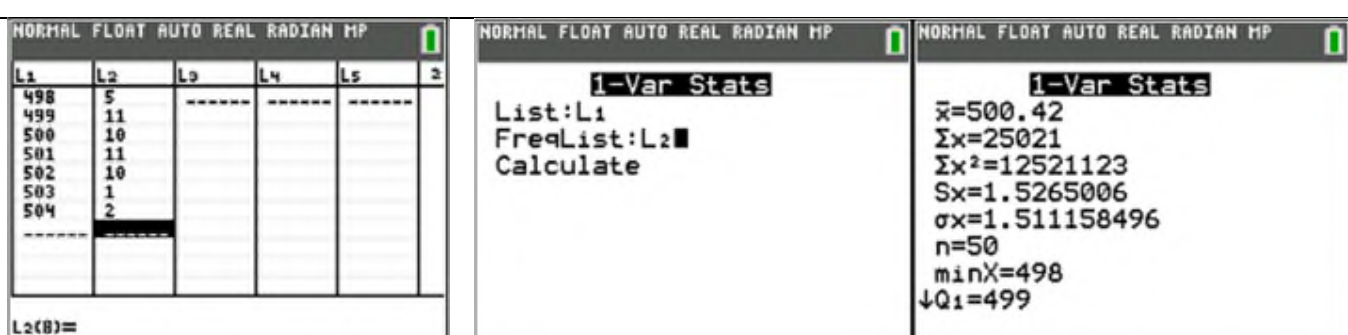
\includegraphics[width=0.98\linewidth]{gc_jpjc_1.png}\par}
Using GC,\par
$\bar{x}=500.42$ (exact)\par
$s=1.5265$ (to 5 s.f.)\par
{\centering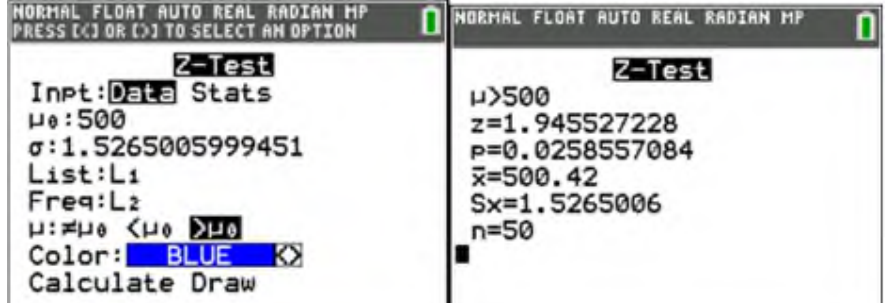
\includegraphics[width=0.66\linewidth]{gc_jpjc_2.png}\par}
Let $X$ = vol. of green tea dispensed in a bottle and\par
\quad $\mu$ = population mean green tea dispensed in a bottle\par
$\mathrm{H}_0:\mu=500$\par
$\mathrm{H}_1:\mu>500$\par
Under $\mathrm{H}_0$ ,since $n$ = 50 is large, by Central Limit Theorem,\par
\qquad $\bar{X}\sim\mathrm{N}\left(500\ ,\ \dfrac{1.5265^2}{50}\right)$ approximately\par
Test statistic: $z=\dfrac{\bar{x}-500}{\left(\dfrac{1.5265}{\sqrt{50}}\right)}$\par
\qquad\qquad\quad $=\dfrac{500.42-500}{\left(\dfrac{1.5265}{\sqrt{50}}\right)}=1.9455\approx1.95$ (to 3 s.f)\par
From GC, $p$-value = $0.025856\approx0.0259$ (to 3 s.f)
\htz{none}{1.9455}{}{1.95}{}{0.0259}
Since $p$-value = 0.0259 $>$ 0.02, we do not reject $\mathrm{H}_0$ at 2\% level of significance and conclude that there is insufficient evidence that the production manager's suspicion is valid.\par\medskip
The $p$-value is 0.0259 and it means there is a probability of 0.0259 of observing a test statistic, $z\geq1.95$, given that the population mean green tea dispensed in a bottle is 500ml.
\pt{(i)} For the production manager's suspicion ($\mu>500$) to be valid, $\mathrm{H}_0$ is rejected. Hence,\par
$p$-value = $0.025856<\dfrac{\alpha}{100}$\par
\qquad $\therefore2.59<\alpha<100$ (3 s.f)
\pt{(ii)} Since the sample size = 50 is large enough, Central Limit Theorem can be applied for sample means to follow a normal distribution approximately.
\pt{(b)} $s^2=\dfrac{n}{n-1}\sigma_x^{\,2}=\dfrac{50}{49}k^2$\par
$\mathrm{H}_0:\mu=500$\par
$\mathrm{H}_1:\mu\neq500$\par
Under $\mathrm{H}_0$ ,since $n$ = 50 is large, by Central Limit Theorem,\par
\qquad $\bar{X}\sim\mathrm{N}\left(500\ ,\ \dfrac{\left(\frac{50k^2}{49}\right)}{50}\right)=\mathrm{N}\left(500\ ,\ \dfrac{k^2}{49}\right)$ approximately\par
Test statistic: $z=\dfrac{\bar{x}-500}{\sqrt{\dfrac{k^2}{49}}}=\dfrac{502-500}{\dfrac{k}{7}}=\dfrac{14}{k}$\par
For $\alpha$ = 0.05,
\htz{-1.95996}{1.95996}{$-1.95996$}{$1.95996$}{}{}
If recalibration is done accurately ($\mu=500$), $\mathrm{H}_0$ is not rejected. Hence,\par
$-1.95996<z<1.95996$\par
\qquad $-1.95996<\dfrac{14}{k}<1.95996$\par
$\dfrac{k}{14}<-0.51021$ (rejected) \ or \ $\dfrac{k}{14}>0.51021$\par
\qquad\qquad\qquad\qquad\qquad\qquad $k>7.1430$\par
\qquad\qquad\qquad\qquad\qquad $\therefore k>7.14$ \ (to 3 s.f)\par\smallskip
{\color{black!55}\footnotesize[Note: the official solution labels the parts 10(i), (ii), (iii), (b); they are shown here as (a), (i), (ii), (b) to match the question's parts. The calculator screens above are the official screenshots printed in the solution.]}
}
%Q 26|CJC 2025 Prelim P2 Q11
\defQ{26}{}{%
EastHam is a football club in a competitive league. It is found that the average time taken by EastHam to score their first goal in a match is 50 minutes. The coach trialled a new play tactic and the time taken, $x$ minutes, to score the first goal is recorded for a random sample of 35 matches in the season. The total time taken is found to be 1650 minutes and the variance of the time is 250 minutes\textsuperscript{2}.\par
The coach wants to test if the average time taken to score the first goal has decreased with the implementation of the new play tactic.
\begin{qparts}
\pt{(a)} Explain why the coach is able to carry out a hypothesis test without any assumption about the distribution of the time taken to score the first goal. \mk{1}
\pt{(b)} Find unbiased estimates of the population mean and variance. Give your answers correct to 3 decimal places. \mk{2}
\pt{(c)} Carry out the test at 10\% level of significance. You should state your hypotheses and define any symbols you use. \mk{4}
\end{qparts}
A fan of another football club in the same league, NewPalace, claims that the average time taken by NewPalace to score their first goal in a match is 40 minutes. The time taken by NewPalace to score the first goal in a match can be assumed to be normally distributed with variance 280 minutes\textsuperscript{2}.
\begin{qparts}
\pt{(d)} A random sample of 50 matches is taken and a hypothesis test is carried out on whether the fan's claim is valid. Find the range of values of the mean time of this sample for which the fan's claim would be rejected at 10\% level of significance. \mk{4}
\end{qparts}
\src{CJC 2025 Prelim P2 Q11}}
\defS{26}{%
\pt{(a)} The sample mean time for 35 matches is approximated to have a normal distribution by the Central Limit Theorem, since sample size is sufficiently large. Hence there is no need to make any assumptions about the distribution of the time taken to score the first goal.
\pt{(b)} Unbiased estimate for population mean $=\dfrac{1650}{35}=47.143$ (to 3d.p.)\par
Unbiased estimate for population variance is $s^2=\dfrac{35}{34}(250)=257.353$ (to 3d.p.)
\pt{(c)} Let $X$ be the random variable denoting time taken by EastHam to score the first goal in a match.\par\medskip
$\mathrm{H}_0:\mu=50$\par
$\mathrm{H}_1:\mu<50$, where $\mu$ is the population mean time taken by EastHam to score the first goal in a match\par\medskip
Under $\mathrm{H}_0$,\par
Since $n$ is large,\par
\qquad $\bar{X}\sim\mathrm{N}\left(50,\dfrac{257.353}{35}\right)$ approximately by CLT\par
\qquad $Z=\dfrac{\bar{X}-50}{\sqrt{s^2/n}}\sim\mathrm{N}(0,1)$\par\medskip
Method \textcircled{\scriptsize 1}:\par
By GC, $p$-value $=0.146$ (3 s.f.).\par
Since $p$-value $>$ 0.1, we do not reject $\mathrm{H}_0$ and conclude that there is insufficient evidence at 10\% significance level to say that average time taken by EastHam to score the first goal has decreased.\par\medskip
Method \textcircled{\scriptsize 2}:\par
$z_{\text{test}}=\dfrac{\left(\frac{1650}{35}\right)-50}{\sqrt{\dfrac{4375/17}{35}}}=-1.05366$, \ $z_{\text{critical}}=-1.28155$
\htz{-1.28155}{none}{$-1.28155$}{}{0.1}{}
Since $z_{\text{test}}>z_{\text{critical}}$, we do not reject $\mathrm{H}_0$ and conclude that there is insufficient evidence at 10\% significance level to say that average time taken by EastHam to score the first goal has decreased.
\pt{(d)} Let $Y$ be the random variable denoting time taken by NewPalace to score the first goal in a match.\par\medskip
$\mathrm{H}_0:\mu=40$\par
$\mathrm{H}_1:\mu\neq40$\par\medskip
Under $\mathrm{H}_0$, $\bar{Y}\sim\mathrm{N}\left(40,\dfrac{280}{50}\right)$
\htz{-1.6449}{1.6449}{$-1.6449$}{$1.6449$}{0.05}{0.05}
Since $\mathrm{H}_0$ is rejected,\par
\qquad $\dfrac{\bar{y}-40}{\sqrt{280/50}}<-1.6449$ \qquad or \qquad $\dfrac{\bar{y}-40}{\sqrt{280/50}}>1.6449$\par
\qquad\qquad $\bar{y}<36.1$ (3 s.f.) \qquad\quad or \qquad\qquad $\bar{y}>43.9$ (3 s.f.)\par
Hence, range of values of $\bar{y}$ is: \ $0<\bar{y}<36.1$ \ or \ $\bar{y}>43.9$\par\smallskip
{\color{black!55}\footnotesize[Note: the official answer key also contains Examiners' Feedback boxes; only the worked solutions are reproduced here.]}
}
%Q 27|HCI 2025 Prelim P2 Q8
\defQ{27}{}{%
A food producer claims that the mean mass of a can of beans it produces is 425 g. Following customer feedback, the production manager wishes to test if the mean mass of a can of beans is indeed 425 g.\par
The production manager took a random sample of size 50 and the mass of each can, in $x$ g, is recorded and the results are shown below:
\[\textstyle\sum x=21209,\ \ \sum(x-424.18)^2=522\]
\begin{qparts}
\pt{(a)} State what it means for a sample to be random in this context. \mk{1}
\pt{(b)} Find the unbiased estimates for the population mean and variance. \mk{2}
\pt{(c)} State the hypotheses for the manager's test, defining any parameters you use. Carry out the test at the 5\% level of significance, giving your conclusion in the context of the question. \mk{5}
\end{qparts}
The production manager wishes to test whether the mean mass of a can of beans has increased using the alternative manufacturing process. He finds that the mean mass of 55 randomly chosen cans is 426.5 g. He carries out a hypothesis test at 10\% level of significance.
\begin{qparts}
\pt{(d)} Explain, with justification, how the population standard deviation of the mass of a can produced under the alternative process will affect the conclusion made by the production manager. \mk{3}
\end{qparts}
\src{HCI 2025 Prelim P2 Q8}}
\defS{27}{%
\pt{(a)} Every can in the population has an equal chance of being selected and is selected independently of the others.
\pt{(b)} Unbiased estimate for the population mean\par
$\bar{x}=\dfrac{\sum x}{50}=\dfrac{21209}{50}=424.18$\par\medskip
Unbiased estimate for the population variance\par
$s^2=\dfrac{50}{50-1}\,\dfrac{\sum(x-\bar{x})^2}{50}$\par
$\phantom{s^2}=\dfrac{\sum(x-424.18)^2}{49}$\par
$\phantom{s^2}=\dfrac{522}{49}$ or 10.65306122
\pt{(c)} Let $X$ be the mass (in grams) of a can of beans.\par
Let $\mu$ and $\sigma^2$ be the population mean and variance of $X$.\par\medskip
$\mathrm{H}_0:\mu=425$\par
$\mathrm{H}_1:\mu\neq425$\par\medskip
$n=50$, $\bar{x}=424.18$, $s^2=\dfrac{522}{49}$\par
Under $\mathrm{H}_0$, since $n=50$ is large, by the Central Limit Theorem ,\par
\qquad $\bar{X}\sim\mathrm{N}\left(425,\dfrac{\sigma^2}{n}\right)$ approximately.\par
Test statistic $Z=\dfrac{\bar{X}-\mu}{\sqrt{\dfrac{S^2}{n}}}\sim\mathrm{N}(0,1)$ approximately\par\medskip
Level of significance: 5\%\par
Reject $\mathrm{H}_0$ if $p$-value $\leq0.05$\par\medskip
Assuming $\mathrm{H}_0$ is true, by G.C., $p$-value $=\mathbf{0.0757}$ (3 s.f.)\par
Since $p$-value$=0.0757>0.05$, we do not reject $\mathrm{H}_0$ at 5\% level of significance and conclude that there is insufficient evidence to say that the population mean mass of a can of beans is not 425 g.
\pt{(d)} Let $Y$ be the mass (in grams) of a can of beans produced using the alternative process.\par
Let $\mu$ and $\sigma^2$ be the population mean and variance of $Y$.\par\medskip
$\mathrm{H}_0:\mu=425$\par
$\mathrm{H}_1:\mu>425$\par
$n=55$, $\bar{y}=426.5$\par\medskip
Under $\mathrm{H}_0$, since $n=55$ is large, by the Central Limit Theorem, $\bar{Y}\sim\mathrm{N}\left(425,\dfrac{\sigma^2}{n}\right)$ approximately.\par
Test statistic $Z=\dfrac{\bar{Y}-\mu}{\sqrt{\dfrac{\sigma^2}{n}}}\sim\mathrm{N}(0,1)$ approximately\par\medskip
Level of significance: 10\%\par
Reject $\mathrm{H}_0$ if $z\geq1.281551567$
\htz{none}{1.281551567}{}{1.2816}{}{0.10}
$\dfrac{426.5-425}{\sqrt{\dfrac{\sigma^2}{55}}}\geq1.281551567$\par
Since $\sigma\geq0$, $\sqrt{\sigma^2}\leq\dfrac{1.5\sqrt{55}}{1.281551567}$\par
\qquad $\Leftrightarrow\sigma\leq8.680335632$\par
\qquad $\Leftrightarrow\sigma\leq8.68$ (3 s.f.)\par
\qquad $\Leftrightarrow0<\sigma\leq8.68$ (3 s.f.)\par\medskip
At 10\% level of significance, if $0<\sigma\leq8.68$ , then $\mathrm{H}_0$ is rejected and the production manager may conclude that mean mass of a can of beans produced using the alternative process has increased.
}

%Q 28|VJC 2025 Prelim P2 Q11
\defQ{28}{}{%
An energy company is studying the relationship between the average daily temperature, $x$ (in degrees Celsius), and the amount of electricity consumed, $y$ (in megawatt-hours MWh). For a random sample of ten days, the records are shown in the table below.\par\smallskip
{\centering\small\begin{tabular}{|l|*{10}{c|}}\hline
\begin{tabular}{@{}l@{}}Average daily temperature\\($x^{\circ}$C)\end{tabular} & 20 & 22 & 24 & 26 & 28 & 30 & 32 & 34 & 36 & 38\\\hline
\begin{tabular}{@{}l@{}}Electricity consumption\\($y$ MWh)\end{tabular} & 12.5 & 12.8 & 13.2 & 14.0 & 14.7 & 16.2 & 16.2 & 19.9 & 22.3 & 29.5\\\hline\end{tabular}\par}
\begin{qparts}
\pt{(a)} Draw a scatter diagram for these values, labelling the axes clearly. \mk{1}
\end{qparts}
It is thought that the electricity consumption and average daily temperature can be modelled by one of the formulae
\[y=a+bx^2,\qquad y=c+dx,\]
where $a$, $b$, $c$ and $d$ are constants.
\begin{qparts}
\pt{(b)} Find the value of the product moment correlation coefficient between\par
\quad\textbf{(i)} $x$ and $y$,\par
\quad\textbf{(ii)} $x^2$ and $y$. \mk{2}
\pt{(c)} Using your answers in parts \textbf{(a)} and \textbf{(b)}, explain which of $y=a+bx^2$ and $y=c+dx$ is the better model and find the equation of a suitable regression line for this model. \mk{3}
\pt{(d)} Use the equation of your regression line to estimate the electricity consumption on a day with an average temperature of $37^{\circ}$C. Comment on the reliability of your estimate. \mk{2}
\end{qparts}
In some regions, temperature is measured in degrees Fahrenheit instead of degrees Celsius. A temperature of $C$ degrees Celsius is equivalent to $F$ degrees Fahrenheit, where $F=\frac{9}{5}C+32$.
\begin{qparts}
\pt{(e)} Rewrite the equation of your regression line found in part \textbf{(c)} in terms of $y$ and $F$, where $F$ is the average daily temperature in degrees Fahrenheit. \mk{1}
\end{qparts}
\src{VJC 2025 Prelim P2 Q11}}
\defS{28}{%
\pt{(a)}\figVjcFiveA
\pt{(b)(i)} From GC, $r=0.89056\approx0.891$.
\pt{(b)(ii)} From GC, $r=0.92229\approx0.922$.
\pt{(c)} From the scatter diagram, it is observed that as $x$ increases, $y$ increases by increasing amounts, and the product moment correlation coefficient between $x^2$ and $y$ is 0.922, which is closer to 1 than that between $x$ and $y$, which is 0.891 . Hence $y=a+bx^2$ is the better model.\par\medskip
$a=4.8291\approx4.83$\par
$b=0.014074\approx0.0141$\par
$y=4.83+0.0141x^2$
\pt{(d)} $y=4.8291+0.014074(37)^2$\par
\quad $\approx24.1$\par
Since $x=37$ lies within the given range of $x$ values, $20\leq x\leq38$, and the value of $r\approx0.922$ is close to 1, the estimated electricity consumption is reliable.
\pt{(e)} $F=\dfrac{9}{5}x+32\Rightarrow x=\dfrac{5}{9}(F-32)$\par
Replace $x$ by $\dfrac{5}{9}(F-32)$:\par
$y=4.8291+0.014074\left[\dfrac{5}{9}(F-32)\right]^2$\par
$\phantom{y}=4.8291+0.0043438(F-32)^2$\par
$\phantom{y}\approx4.83+0.00434(F-32)^2$
}
%Q 29|VJC 2024 Prelim P2 Q10
\defQ{29}{}{%
The yield per hectare, $y$ kg, of a crop is believed to depend on the average rainfall, $x$ mm, in the month of June. For 10 regions, records are kept of the values of $x$ and $y$, and these are shown in the table below. The yield from the tenth region was accidentally deleted from the records after the data was analysed, and this is indicated by the value $p$.\par\smallskip
{\centering\small\begin{tabular}{|l|*{10}{c|}}\hline
\begin{tabular}{@{}l@{}}Average rainfall\\($x$ mm)\end{tabular} & 149 & 110 & 188 & 135 & 156 & 140 & 168 & 118 & 122 & 174\\\hline
\begin{tabular}{@{}l@{}}Yield of crop\\($y$ kg)\end{tabular} & 13.8 & 6.5 & 15.2 & 12.2 & 14.4 & 12.2 & 14.7 & 9.5 & 9.9 & $p$\\\hline\end{tabular}\par}\smallskip
Given that the equation of the regression line of $y$ on $x$ is $y=-2.5652+0.10168x$, show that $p=14.4$. \mk{2}
\begin{qparts}
\pt{(a)} Draw a scatter diagram for these values, labelling the axes clearly. Calculate the product moment correlation coefficient between $x$ and $y$. \mk{2}
\pt{(b)} It is thought that a model of the form $y=a+b\ln x$ may also be a suitable fit to the data. Calculate least square estimates of $a$ and $b$, and find the value of the product moment correlation coefficient between $y$ and $\ln x$. \mk{3}
\pt{(c)} Use your answers to parts \textbf{(a)} and \textbf{(b)} to explain which of
\[y=-2.5652+0.10168x\ \text{ or }\ y=a+b\ln x\]
is the better model. \mk{2}
\pt{(d)} Using an appropriate regression line, estimate the yield for a region that experienced 200 mm of rainfall in June. Comment on the reliability of your estimate. \mk{2}
\pt{(e)} In some regions, rainfall is measured in inches instead of in mm. Given that there are 25.4 mm in an inch, show how the regression line found in part \textbf{(b)} can be re-written so that it can be used when $x$, the average rainfall in June, is given in inches. \mk{1}
\end{qparts}
\src{VJC 2024 Prelim P2 Q10}}
\defS{29}{%
\pt{(Show)} $\sum x=1460$, $\sum y=108.4+p$, $n=10$\par
Since $(\bar{x},\bar{y})$ lies on the regression line of $y$ on $x$,\par
\qquad $\bar{y}=-2.5652+0.10168\bar{x}$\par
$\dfrac{108.4+p}{10}=-2.5652+0.10168\dfrac{1460}{10}$\par
\qquad\qquad $=12.28008$\par
\qquad\quad $p=14.4008$\par
\qquad\quad\ \ $\approx14.4$ \ (shown)
\pt{(a)}\figVjcFourA
From GC,\par
product moment correlation coefficient, $r=0.92147\approx0.921$
\pt{(b)} From GC, the regression line of $y$ on $\ln x$ is\par
$y=-63.028+15.154\ln x$\par
$a=-63.028\approx-63.0$\par
$b=15.154\approx15.2$\par
$r=0.94660\approx0.947$
\pt{(c)} 1) From the scatter diagram, it is observed that as $x$ increases, $y$ increases by decreasing amounts, and\par
2) product moment correlation coefficient between $y$ and $\ln x$ is 0.947, which is closer to 1 than that of $x$ and $y$, which is 0.921 .\par
Hence $y=a+b\ln x$ is the better model.
\pt{(d)} $y=-63.028+15.154\ln200$\par
\quad $=17.262$\par
\quad $\approx17.3$\par\medskip
Since $x=200$ lies outside the given range of $x$ values, $110\leq x\leq188$, the estimated yield may not be reliable.
\pt{(e)} Replace $x$ by $25.4x$,\par
$y=-63.028+15.154\ln(25.4x)$\par
$\phantom{y}=-63.028+15.154[\ln25.4+\ln x]$\par
$\phantom{y}=-14.009+15.154\ln x$\par
$\phantom{y}=-14.0+15.2\ln x$\par\smallskip
{\color{black!55}\footnotesize[Note: the official solution also has a ``Comments'' column (marking tips); only the Solutions column is reproduced here.]}
}
%Q 30|9758 A-Level 2024 P2 Q11
\defQ{30}{}{%
\begin{qparts}
\pt{(a)} A certain brand of breakfast cereal is sold in a variety of different sized packs. Details of the mass of cereal in each pack, $m$ grams, and the price, $p$ cents, are given in the table below.\par\smallskip
{\centering\begin{tabular}{|c|c|c|c|c|c|c|}\hline $m$ & 24 & 250 & 550 & 1000 & 2000 & 5000\\\hline $p$ & 100 & 300 & 400 & 600 & 900 & 1200\\\hline\end{tabular}\par}\smallskip
A scatter diagram for the data is shown below.
\figALcereal
\pt{(i)} Explain what the scatter diagram tells you about the relationship between $m$ and $p$. \mk{1}
\end{qparts}
The following two models are proposed, where $a$, $b$, $d$ and $e$ are constants.
\[p=a+b\ln m\qquad\qquad p=d+e\sqrt{m}\]
\begin{qparts}
\pt{(ii)} Determine which of these models gives the better fit to the data. State the values of the constants and the product moment correlation coefficient in this case. \mk{4}
\pt{(iii)} A new pack containing 750 grams of cereal is introduced. Use the model you identified in part \textbf{(a)(ii)} to estimate the price of this pack, correct to the nearest 10 cents. Explain whether your answer is reliable. \mk{2}
\pt{(b)} Kai is investigating the relationship between the number, $n$, of a particular type of high-performance batteries in a pack and the price, \$$y$, of the pack she found in different stores. Her results are shown in the table below.\par\smallskip
{\centering\begin{tabular}{|c|c|c|c|c|c|}\hline $n$ & 2 & 5 & 6 & 7 & 11\\\hline $y$ & 6 & 10 & 16 & 20 & 25\\\hline\end{tabular}\par}\smallskip
This information is shown in the scatter diagram below.
\figALkai
Kai decides to investigate whether the model $y=\frac52n+1$ is a good fit for this data.
\pt{(i)} Draw the line $y=\frac52n+1$ on the scatter diagram above. \mk{1}
\pt{(ii)} For the model $y=\mathrm{f}(n)$, the residual for a point $(a,b)$ is $b-\mathrm{f}(a)$.\par
\textbf{(A)} Mark the residuals for the points on the scatter diagram above. \mk{1}\par
\textbf{(B)} Explain why Kai should use the sum of the squares of the residuals rather than the sum of the residuals when assessing the fit of the model. \mk{1}\par
\textbf{(C)} Calculate the sum of the squares of the residuals for the line $y=\frac52n+1$. \mk{1}
\end{qparts}
Kai's friend points out that other lines parallel to Kai's line can be drawn which are a better fit for the data.
\begin{qparts}
\pt{(iii)} Explain how the sum of the squares of the residuals for a line that is a better fit for the data differs from the sum of the squares of the residuals for the line $y=\frac52n+1$ found in part \textbf{(ii)(C)}. \mk{1}
\pt{(iv)} Find the range of values of $c$ for which the line $y=\frac52n+c$ is a better fit for the data than the line $y=\frac52n+1$. \mk{3}
\end{qparts}
\src{9758 A-Level 2024 P2 Q11}}
\defS{30}{%
\pt{(a)(i)} The scatter diagram tells us that as mass of a pack of cereal ($m$) increases, the price ($p$) increases at a decreasing rate.
\pt{(a)(ii)} For $p=a+b\ln m$, product moment correlation coefficient $r_1=0.928513$\par
For $p=d+e\sqrt{m}$, product moment correlation coefficient $r_2=0.991438$\par
Since $r_2$ is closer to 1 than $r_1$, the model \underline{$p=d+e\sqrt{m}$} gives a better fit to the data.\par\medskip
For this model, $d=32.952567=\underline{33.0}$ and $e=17.269804=\underline{17.3}$\par
$r=r_2=\underline{0.991}$ (all answers to 3 s.f.)
\pt{(a)(iii)} $p=32.952567+17.269804\sqrt{m}$\par
Sub. $m=750$:\par
$p=32.952567+17.269804\sqrt{750}$\par
\quad $=505.906$\par
$\therefore$ Estimated price $=\underline{510\text{ cents}}$ (nearest 10 cents)\par\medskip
This estimate is reliable as the product moment correlation coefficient of 0.991 is very close to 1, indicating a strong positive linear correlation between $\sqrt{m}$ and $p$. Furthermore, the value $m=750$ is within the data range $24\leq m\leq5000$, hence the estimate is an interpolation.
\pt{(b)(i)}\figALkaiSol
\pt{(b)(ii)(A)}{\centering\setlength{\tabcolsep}{4pt}\begin{tabular}{|l|c|c|c|c|c|}\hline
Point $(a,b)$ & (2, 6) & (5, 10) & (6, 16) & (7, 20) & (11, 25)\\\hline
$\mathrm{f}(a)$ & 6 & 13.5 & 16 & 18.5 & 28.5\\\hline
Residual $b-\mathrm{f}(a)$ & 0 & $-3.5$ & 0 & 1.5 & $-3.5$\\\hline\end{tabular}\par}
\pt{(b)(ii)(B)} As residuals may be positive or negative (or zero), they may cancel out if Kai simply sums the residuals. Squaring the residuals allows Kai to sum up positive numbers for a more accurate assessment of the fit of the model.
\pt{(b)(ii)(C)} Sum of squares of residuals for the line $y=\frac52n+1$ is $0^2+(-3.5)^2+0^2+1.5^2+(-3.5)^2=\underline{26.75}$
\pt{(b)(iii)} The sum of squares of residuals for a line that is a better fit will be less than the sum of squares of residuals for the line $y=\frac52n+1$, i.e. less than 26.75.
\pt{(b)(iv)} Consider $\mathrm{f}(n)=\frac52n+c$.\par\smallskip
{\centering\setlength{\tabcolsep}{4pt}\begin{tabular}{|l|c|c|c|c|c|}\hline
Point $(a,b)$ & (2, 6) & (5, 10) & (6, 16) & (7, 20) & (11, 25)\\\hline
$\mathrm{f}(a)$ & $5+c$ & $12.5+c$ & $15+c$ & $17.5+c$ & $27.5+c$\\\hline
Residual $b-\mathrm{f}(a)$ & $1-c$ & $-2.5-c$ & $1-c$ & $2.5-c$ & $-2.5-c$\\\hline\end{tabular}\par}\smallskip
Sum of squares of residuals for the line $y=\frac52n+c$ is\par
$(1-c)^2+(-2.5-c)^2+(1-c)^2+(2.5-c)^2+(-2.5-c)^2$\par
$=2(1-c)^2+2(2.5+c)^2+(2.5-c)^2$\par
$=20.75+c+5c^2$\par\medskip
For this to be a better fit,\par
$20.75+c+5c^2<26.75$\par
$5c^2+c-6<0$
\figALparab
Using GC, range of values of $c$ is \underline{$-1.2<c<1$}\par\smallskip
{\color{black!55}\footnotesize[Note: SEAB publishes no worked solutions. This is the worked solution from the local file ``2024 GCE A-Level H2 Mathematics 9758 Paper 2 Solutions'' (tmp\_ch10/AL2024\_P2\_with\_sol.pdf); its author is not named on the document.]}
}
%Q 31|9758 A-Level 2019 P2 Q10
\defQ{31}{}{%
Abi and Bhani find the fuel consumption for a car driven at different constant speeds. The table shows the fuel consumption, $y$ kilometres per litre, for different constant speeds, $x$ kilometres per hour.\par\smallskip
{\centering\begin{tabular}{|c|c|c|c|c|c|}\hline $x$ & 40 & 45 & 50 & 55 & 60\\\hline $y$ & 22 & 20 & 18 & 17 & 16\\\hline\end{tabular}\par}
\begin{qparts}
\pt{(i)} Abi decides to model the data using the line $y=35-\frac13x$.\par
\textbf{(a)} On the grid\par
\qquad$\bullet$ draw a scatter diagram of the data,\par
\qquad$\bullet$ draw the line $y=35-\frac13x$. \mk{2}
\figAbiGrid
\textbf{(b)} For a line of best fit $y=\mathrm{f}(x)$, the residual for a point $(a,b)$ plotted on the scatter diagram is the vertical distance between $(a,\mathrm{f}(a))$ and $(a,b)$. Mark the residual for each point on your diagram. \mk{1}\par
\textbf{(c)} Calculate the sum of the squares of the residuals for Abi's line. \mk{1}\par
\textbf{(d)} Explain why, in general, the sum of the squares of the residuals rather than the sum of the residuals is used. \mk{1}
\end{qparts}
Bhani models the same data using a straight line passing through the points (40, 22) and (55, 17).\par
The sum of the squares of the residuals for Bhani's line is 1.
\begin{qparts}
\pt{(ii)} State, with a reason, which of the two models, Abi's or Bhani's, gives a better fit. \mk{1}
\pt{(iii)} State the coordinates of the point that the least squares regression line must pass through. \mk{1}
\pt{(iv)} Use your calculator to find the equation of the least squares regression line of $y$ on $x$. State the value of the product moment correlation coefficient. \mk{3}
\pt{(v)} Use the equation of the regression line to estimate the fuel consumption when the speed is 30 kilometres per hour. Explain whether you would expect this value to be reliable. \mk{2}
\pt{(vi)} Cerie performs a similar experiment on a different car. She finds that the sum of the squares of the residuals for her line is 0. What can you deduce about the data points in Cerie's experiment? \mk{1}
\end{qparts}
\src{9758 A-Level 2019 P2 Q10}}
\defS{31}{%
\pt{(i)(a)}\figAbiSol
\pt{(i)(b)} The residuals are the distances labelled $e_1,\ldots,e_5$ in the diagram.
\pt{(i)(c)} $\displaystyle\sum_{i=1}^{5}(e_i)^2=\frac19+0+\frac19+\frac19+1=\frac43$\par\smallskip
Key the eqn in Y$_1$ \quad Define L$_3$ = Y$_{\text{estimated}}$ \quad Define L$_4$ = $e_i^2$\par
Optional : Using List to calculate the Sum\par
Go to List (Type 2nd $\rightarrow$ stat $\rightarrow$ MATH) \quad Sum all the entries in L$_4$
\pt{(i)(d)} Residuals can be positive or negative since they are calculated by taking (\textit{the observed y-value}) -- (\textit{the estimated y-value}). Taking the sum of these residuals will result in them cancelling out and thus losing important information. Taking the sum of the squares of the residuals will avoid this problem.
\pt{(ii)} Sum of the squares of the residuals for Bhani's model $=1<\dfrac43$ (Sum of the squares of the residuals for Abi's model), Bhani's model is a better fit.
\pt{(iii)} $(\bar{x},\bar{y})=(50,\,18.6)$
\pt{(iv)} Regression line: $y=-0.3x+33.6$\par
$r=-0.985$ (3 s.f.)
\pt{(v)} $x=30$ , $y=24.6$ (kilometres per litre)\par
$x=30$ is outside the given range of $x$-values. The estimate obtained using extrapolation is unreliable.
\pt{(vi)} Sum of the squares of the residuals = 0 implies that ALL data points lie on the regression line, which is highly unlikely in a real-life experiment.\par\smallskip
{\color{black!55}\footnotesize[Note: SEAB publishes no worked solutions. This is the Raffles Institution ``Solution for 2019 A-Level Paper 2'' (grail.moe item 19456). Its small GC screenshots for (i)(c) are illegible in the source and are described in words only. Question text transcribed from a tutor compilation (Paradigm ``Correlation and Regression'', Q7 N2019/P2/Q10), as no local copy of the SEAB question paper was found.]}
}

\begin{document}
\makeatletter\setbox0\vbox{\@starttoc{toc}}\makeatother
\IfFileExists{stats_ex_front.tex}{\thispagestyle{empty}\noindent\colorbox{blue!50!black}{\parbox{\dimexpr\textwidth-2\fboxsep}{\vspace{5mm}\hspace*{4mm}{\color{white}\fontsize{28}{32}\selectfont\bfseries Syllabus 9758 Statistics}\\[2mm]\hspace*{4mm}{\color{white}\Large Example Questions}\vspace{4mm}}}\par\vspace{2mm}\noindent{\color{teal!50!black}\rule{\textwidth}{1.2pt}}\par\vspace{1mm}\noindent{\large Maximus Pung}\par\vspace{5mm}
\noindent{\fontsize{22}{26}\selectfont\color{blue!50!black} Contents\par}\vspace{3mm}
{\small\linespread{0.92}\selectfont
\medskip\noindent\colorbox{blue!8}{\parbox{\dimexpr\textwidth-2\fboxsep}{\large\bfseries\color{blue!50!black}\colorbox{blue!50!black}{\color{white}\,1\,}\quad Permutations and Combinations\hfill 3}}\par\nopagebreak\smallskip\nopagebreak
\noindent\hspace*{2em}{\color{teal!50!black}\bfseries Question 1.1}\quad Choosing with ``at least'' conditions; circular arrangements\dotfill\ 3\par
\noindent\hspace*{2em}{\color{teal!50!black}\bfseries Question 1.2}\quad Probabilities from a table; access codes from BOOKKEEPER; ``at least one from each group''\dotfill\ 5\par
\noindent\hspace*{2em}{\color{teal!50!black}\bfseries Question 1.3}\quad Choosing teams (football)\dotfill\ 8\par
\noindent\hspace*{2em}{\color{teal!50!black}\bfseries Question 1.4}\quad Arranging in rows ($2\times n$); round table\dotfill\ 10\par
\medskip\noindent\colorbox{blue!8}{\parbox{\dimexpr\textwidth-2\fboxsep}{\large\bfseries\color{blue!50!black}\colorbox{blue!50!black}{\color{white}\,2\,}\quad Probability\hfill 12}}\par\nopagebreak\smallskip\nopagebreak
\noindent\hspace*{2em}{\color{teal!50!black}\bfseries Question 2.1}\quad Tree diagram\dotfill\ 12\par
\noindent\hspace*{2em}{\color{teal!50!black}\bfseries Question 2.2}\quad Sampling; Venn diagram: range of values of a probability\dotfill\ 14\par
\noindent\hspace*{2em}{\color{teal!50!black}\bfseries Question 2.3}\quad Sum to infinity of a GP; distribution of a score; fair game\dotfill\ 17\par
\noindent\hspace*{2em}{\color{teal!50!black}\bfseries Question 2.4}\quad Contextual probability\dotfill\ 19\par
\medskip\noindent\colorbox{blue!8}{\parbox{\dimexpr\textwidth-2\fboxsep}{\large\bfseries\color{blue!50!black}\colorbox{blue!50!black}{\color{white}\,3\,}\quad Discrete Random Variables\hfill 21}}\par\nopagebreak\smallskip\nopagebreak
\noindent\hspace*{2em}{\color{teal!50!black}\bfseries Question 3.1}\quad Unknowns in the table; solving simultaneously\dotfill\ 21\par
\noindent\hspace*{2em}{\color{teal!50!black}\bfseries Question 3.2}\quad Fair game\dotfill\ 22\par
\noindent\hspace*{2em}{\color{teal!50!black}\bfseries Question 3.3}\quad Total of two games (not CLT)\dotfill\ 24\par
\noindent\hspace*{2em}{\color{teal!50!black}\bfseries Question 3.4}\quad Expectation of a new variable (new table)\dotfill\ 26\par
\noindent\hspace*{2em}{\color{teal!50!black}\bfseries Question 3.5}\quad Central Limit Theorem\dotfill\ 28\par
\medskip\noindent\colorbox{blue!8}{\parbox{\dimexpr\textwidth-2\fboxsep}{\large\bfseries\color{blue!50!black}\colorbox{blue!50!black}{\color{white}\,4\,}\quad Binomial Distribution\hfill 30}}\par\nopagebreak\smallskip\nopagebreak
\noindent\hspace*{2em}{\color{teal!50!black}\bfseries Question 4.1}\quad Double binomial\dotfill\ 30\par
\noindent\hspace*{2em}{\color{teal!50!black}\bfseries Question 4.2}\quad The $k$th trial is the $m$th success\dotfill\ 32\par
\noindent\hspace*{2em}{\color{teal!50!black}\bfseries Question 4.3}\quad Bug turning left and right\dotfill\ 33\par
\noindent\hspace*{2em}{\color{teal!50!black}\bfseries Question 4.4}\quad Range of $p$ given the mode\dotfill\ 34\par
\noindent\hspace*{2em}{\color{teal!50!black}\bfseries Question 4.5}\quad Central Limit Theorem\dotfill\ 35\par
\medskip\noindent\colorbox{blue!8}{\parbox{\dimexpr\textwidth-2\fboxsep}{\large\bfseries\color{blue!50!black}\colorbox{blue!50!black}{\color{white}\,5\,}\quad Normal Distribution\hfill 37}}\par\nopagebreak\smallskip\nopagebreak
\noindent\hspace*{2em}{\color{teal!50!black}\bfseries Question 5.1}\quad Combining independent normal variables\dotfill\ 37\par
\noindent\hspace*{2em}{\color{teal!50!black}\bfseries Question 5.2}\quad Sketching a normal curve\dotfill\ 39\par
\noindent\hspace*{2em}{\color{teal!50!black}\bfseries Question 5.3}\quad invNorm simultaneous equations; $\mitmu $ by symmetry\dotfill\ 41\par
\noindent\hspace*{2em}{\color{teal!50!black}\bfseries Question 5.4}\quad Binomial count of a normal event\dotfill\ 43\par
\medskip\noindent\colorbox{blue!8}{\parbox{\dimexpr\textwidth-2\fboxsep}{\large\bfseries\color{blue!50!black}\colorbox{blue!50!black}{\color{white}\,6\,}\quad Hypothesis Testing\hfill 47}}\par\nopagebreak\smallskip\nopagebreak
\noindent\hspace*{2em}{\color{teal!50!black}\bfseries Question 6.1}\quad Basic test; reverse: smallest significance level, range of variance\dotfill\ 47\par
\noindent\hspace*{2em}{\color{teal!50!black}\bfseries Question 6.2}\quad Data as $\mitSigma (x-k)$ and $\mitSigma (x-k)^2$\dotfill\ 50\par
\noindent\hspace*{2em}{\color{teal!50!black}\bfseries Question 6.3}\quad Data in a frequency table (GC steps)\dotfill\ 53\par
\noindent\hspace*{2em}{\color{teal!50!black}\bfseries Question 6.4}\quad Sample variance given ($\frac {n}{n-1}\times $ sample variance)\dotfill\ 56\par
\noindent\hspace*{2em}{\color{teal!50!black}\bfseries Question 6.5}\quad Data as $\mitSigma x$ and $\mitSigma (x-k)^2$\dotfill\ 59\par
\medskip\noindent\colorbox{blue!8}{\parbox{\dimexpr\textwidth-2\fboxsep}{\large\bfseries\color{blue!50!black}\colorbox{blue!50!black}{\color{white}\,7\,}\quad Correlation and Linear Regression\hfill 62}}\par\nopagebreak\smallskip\nopagebreak
\noindent\hspace*{2em}{\color{teal!50!black}\bfseries Question 7.1}\quad Comparing models (scatter diagram and $r$); estimate and reliability\dotfill\ 62\par
\noindent\hspace*{2em}{\color{teal!50!black}\bfseries Question 7.2}\quad Missing $y$ value from the LSRL via $(\bar x,\bar y)$\dotfill\ 64\par
\noindent\hspace*{2em}{\color{teal!50!black}\bfseries Question 7.3}\quad Sum of squares of residuals\dotfill\ 67\par
\noindent\hspace*{2em}{\color{teal!50!black}\bfseries Question 7.4}\quad Abi and Bhani: residuals and least squares\dotfill\ 71\par
}
}{\thispagestyle{empty}\null}\clearpage
\inchap{Permutations and Combinations}
\qfirst\phantomsection\addcontentsline{toc}{section}{Question \thechapter.\the\numexpr\value{diq}+1\relax\ [TJC 2025 Prelim P2 Q6] --- Choosing with ``at least'' conditions; circular arrangements}\putQS{1}
\qnew\phantomsection\addcontentsline{toc}{section}{Question \thechapter.\the\numexpr\value{diq}+1\relax\ [ASRJC 2025 Prelim P2 Q11] --- Probabilities from a table; access codes from BOOKKEEPER; ``at least one from each group''}\putQS{2}
\qnew\phantomsection\addcontentsline{toc}{section}{Question \thechapter.\the\numexpr\value{diq}+1\relax\ [JPJC 2026 Prelim P2 Q8] --- Choosing teams (football)}\putQS{3}
\qnew\phantomsection\addcontentsline{toc}{section}{Question \thechapter.\the\numexpr\value{diq}+1\relax\ [ASRJC 2024 Prelim P2 Q8] --- Arranging in rows (\texorpdfstring{$2\times n$}{2times n}); round table}\putQS{4}
\clearpage\inchap{Probability}
\qfirst\phantomsection\addcontentsline{toc}{section}{Question \thechapter.\the\numexpr\value{diq}+1\relax\ [EJC 2025 Prelim P2 Q6] --- Tree diagram}\putQS{5}
\qnew\phantomsection\addcontentsline{toc}{section}{Question \thechapter.\the\numexpr\value{diq}+1\relax\ [CJC 2024 Prelim P2 Q10] --- Sampling; Venn diagram: range of values of a probability}\putQS{6}
\qnew\phantomsection\addcontentsline{toc}{section}{Question \thechapter.\the\numexpr\value{diq}+1\relax\ [ACJC 2023 Prelim P2 Q9] --- Sum to infinity of a GP; distribution of a score; fair game}\putQS{7}
\qnew\phantomsection\addcontentsline{toc}{section}{Question \thechapter.\the\numexpr\value{diq}+1\relax\ [HCI 2025 Prelim P2 Q6] --- Contextual probability}\putQS{8}
\sidenote{See also Example 3 (b), (c) for another contextual probability question.}\par
\clearpage\inchap{Discrete Random Variables}
\qfirst\phantomsection\addcontentsline{toc}{section}{Question \thechapter.\the\numexpr\value{diq}+1\relax\ [ACJC 2025 Prelim P2 Q8] --- Unknowns in the table; solving simultaneously}\putQS{9}
\qnew\phantomsection\addcontentsline{toc}{section}{Question \thechapter.\the\numexpr\value{diq}+1\relax\ [ASRJC 2025 Prelim P2 Q7] --- Fair game}\putQS{10}
\qnew\phantomsection\addcontentsline{toc}{section}{Question \thechapter.\the\numexpr\value{diq}+1\relax\ [CJC 2024 Prelim P2 Q5] --- Total of two games (not CLT)}\putQS{11}
\qnew\phantomsection\addcontentsline{toc}{section}{Question \thechapter.\the\numexpr\value{diq}+1\relax\ [SAJC DRV HW2 Review Q8] --- Expectation of a new variable (new table)}\putQS{12}
\sidenote{Only the answer line printed with the question (SAJC DRV HW2 Review Q8) is available; no official worked solution was found.}\par
\qnew\phantomsection\addcontentsline{toc}{section}{Question \thechapter.\the\numexpr\value{diq}+1\relax\ [JPJC 2025 Prelim P2 Q7] --- Central Limit Theorem}\putQS{13}
\clearpage\inchap{Binomial Distribution}
\qfirst\phantomsection\addcontentsline{toc}{section}{Question \thechapter.\the\numexpr\value{diq}+1\relax\ [ACJC 2025 Prelim P2 Q9] --- Double binomial}\putQS{14}
\qnew\phantomsection\addcontentsline{toc}{section}{Question \thechapter.\the\numexpr\value{diq}+1\relax\ [YIJC 2024 Prelim P2 Q8] --- The \texorpdfstring{$k$}{k}th trial is the \texorpdfstring{$m$}{m}th success}\putQS{15}
\qnew\phantomsection\addcontentsline{toc}{section}{Question \thechapter.\the\numexpr\value{diq}+1\relax\ [N2018 P2 Q6] --- Bug turning left and right}\putQS{16}
\sidenote{No official SEAB solution is published; answers as printed with this question in RI 2025 Tutorial S2B Q10.}\par
\qnew\phantomsection\addcontentsline{toc}{section}{Question \thechapter.\the\numexpr\value{diq}+1\relax\ [9758 Specimen Paper (for 2025) P2 Q7] --- Range of \texorpdfstring{$p$}{p} given the mode}\putQS{17}
\qnew\phantomsection\addcontentsline{toc}{section}{Question \thechapter.\the\numexpr\value{diq}+1\relax\ [TJC 2025 Prelim P2 Q7] --- Central Limit Theorem}\putQS{18}
\clearpage\inchap{Normal Distribution}
\qfirst\phantomsection\addcontentsline{toc}{section}{Question \thechapter.\the\numexpr\value{diq}+1\relax\ [ASRJC 2025 Prelim P2 Q9] --- Combining independent normal variables}\putQS{19}
\qnew\phantomsection\addcontentsline{toc}{section}{Question \thechapter.\the\numexpr\value{diq}+1\relax\ [NJC 2024 Prelim P2 Q12] --- Sketching a normal curve}\putQS{20}
\qnew\phantomsection\addcontentsline{toc}{section}{Question \thechapter.\the\numexpr\value{diq}+1\relax\ [MI 2025 Prelim P2 Q6] --- invNorm simultaneous equations; \texorpdfstring{$\mu$}{mu} by symmetry}\putQS{21}
\qnew\phantomsection\addcontentsline{toc}{section}{Question \thechapter.\the\numexpr\value{diq}+1\relax\ [RVHS 2025 Prelim P2 Q12] --- Binomial count of a normal event}\putQS{22}
\clearpage\inchap{Hypothesis Testing}
\qfirst\phantomsection\addcontentsline{toc}{section}{Question \thechapter.\the\numexpr\value{diq}+1\relax\ [ACJC 2023 Prelim P2 Q11] --- Basic test; reverse: smallest significance level, range of variance}\putQS{23}
\qnew\phantomsection\addcontentsline{toc}{section}{Question \thechapter.\the\numexpr\value{diq}+1\relax\ [VJC 2025 Prelim P2 Q12] --- Data as \texorpdfstring{$\Sigma(x-k)$ and $\Sigma(x-k)^2$}{sums of (x-k)}}\putQS{24}
\qnew\phantomsection\addcontentsline{toc}{section}{Question \thechapter.\the\numexpr\value{diq}+1\relax\ [JPJC 2024 Prelim P2 Q10] --- Data in a frequency table (GC steps)}\putQS{25}
\qnew\phantomsection\addcontentsline{toc}{section}{Question \thechapter.\the\numexpr\value{diq}+1\relax\ [CJC 2025 Prelim P2 Q11] --- Sample variance given (\texorpdfstring{$\frac{n}{n-1}\times$}{n/(n-1) x} sample variance)}\putQS{26}
\qnew\phantomsection\addcontentsline{toc}{section}{Question \thechapter.\the\numexpr\value{diq}+1\relax\ [HCI 2025 Prelim P2 Q8] --- Data as \texorpdfstring{$\Sigma x$ and $\Sigma(x-k)^2$}{sum x and sum (x-k)2}}\putQS{27}
\clearpage\inchap{Correlation and Linear Regression}
\qfirst\phantomsection\addcontentsline{toc}{section}{Question \thechapter.\the\numexpr\value{diq}+1\relax\ [VJC 2025 Prelim P2 Q11] --- Comparing models (scatter diagram and \texorpdfstring{$r$}{r}); estimate and reliability}\putQS{28}
\qnew\phantomsection\addcontentsline{toc}{section}{Question \thechapter.\the\numexpr\value{diq}+1\relax\ [VJC 2024 Prelim P2 Q10] --- Missing \texorpdfstring{$y$}{y} value from the LSRL via \texorpdfstring{$(\bar x,\bar y)$}{(xbar,ybar)}}\putQS{29}
\qnew\phantomsection\addcontentsline{toc}{section}{Question \thechapter.\the\numexpr\value{diq}+1\relax\ [9758 A-Level 2024 P2 Q11] --- Sum of squares of residuals}\putQS{30}
\qnew\phantomsection\addcontentsline{toc}{section}{Question \thechapter.\the\numexpr\value{diq}+1\relax\ [9758 A-Level 2019 P2 Q10] --- Abi and Bhani: residuals and least squares}\putQS{31}
\makeatletter\immediate\write\@auxout{}\makeatother
\end{document}
